\chapter{日記アプリケーションの作成(Reactのみ)}
\label{chap:03-todo-with-react}
\begin{reviewimage}[H]%%diary01
\starterimageframe{%
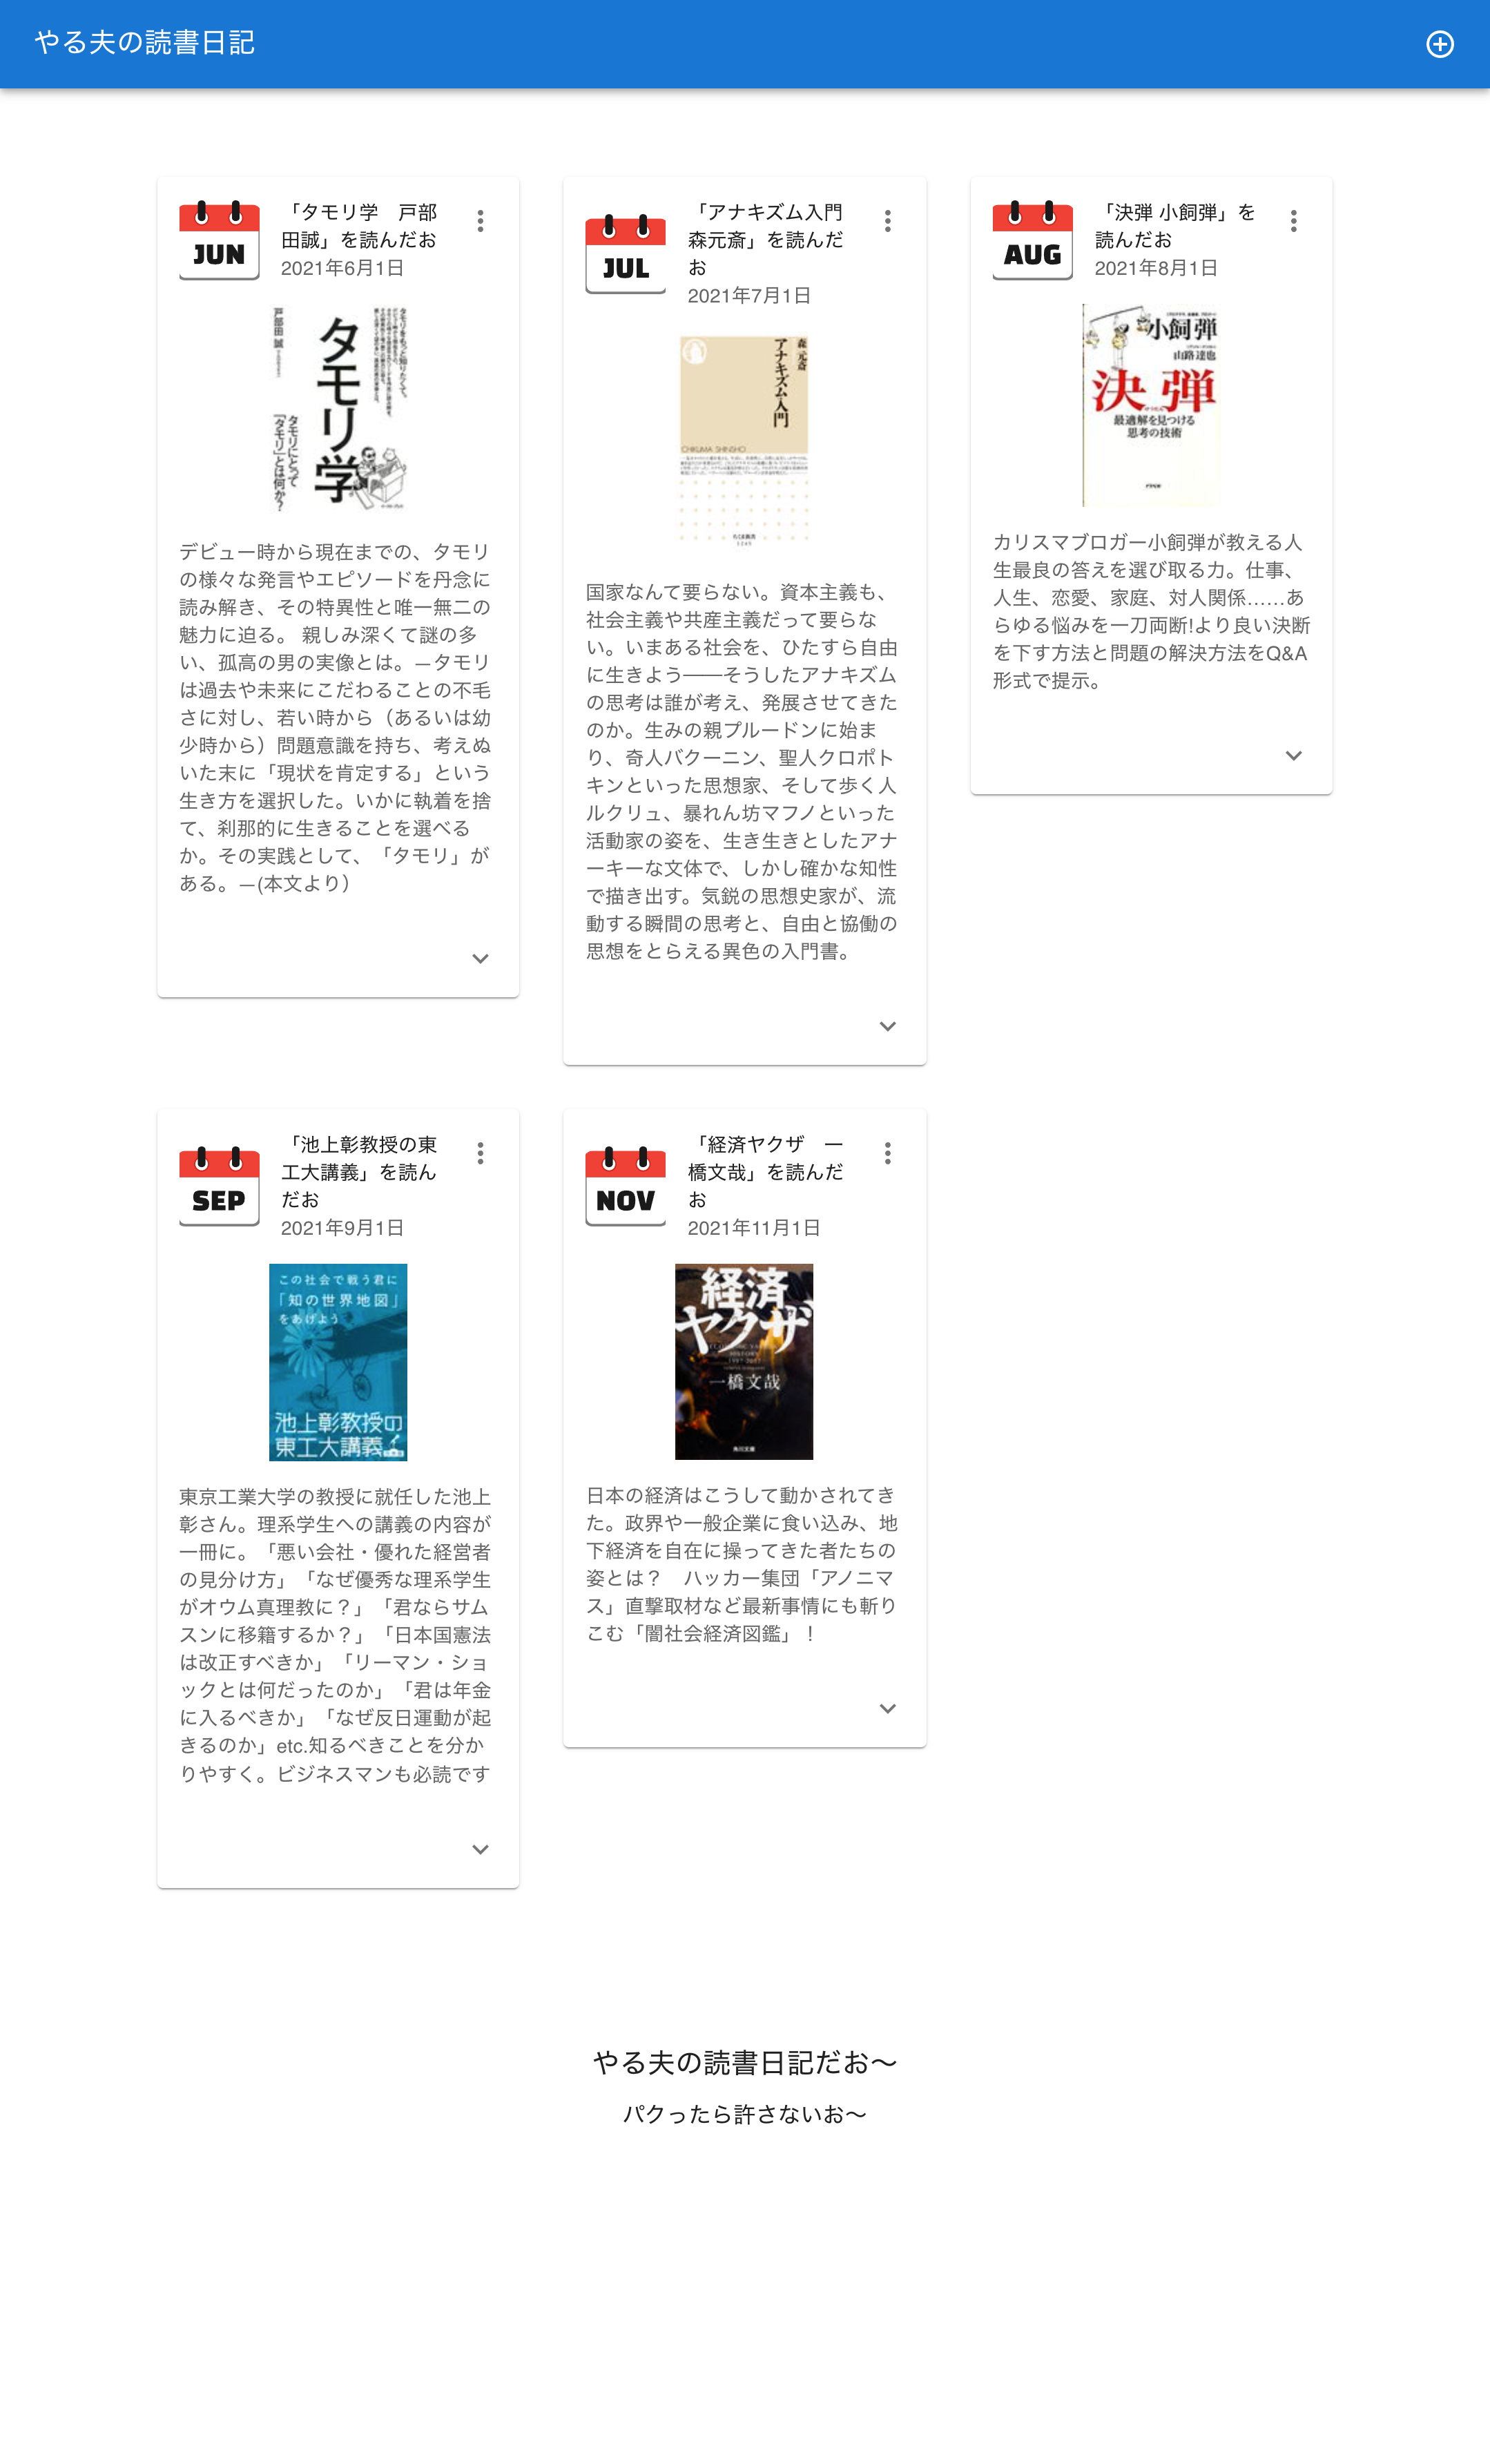
\includegraphics[width=0.5\maxwidth]{./images/03-todo-with-react/diary01.png}%
}%
\reviewimagecaption{完成サンプルアプリケーション}
\label{image:03-todo-with-react:diary01}
\end{reviewimage}
\begin{starterabstract}
  本章では、第2章で作成したスタートアップ用のアプリケーションを魔改造し、日記アプリケーションを作成します。\\[0pt]

  また、表示用のUIには、Googleが提唱するMaterial DesignのReact用UIの最新版MUI5を使用します。
\end{starterabstract}

サンプルアプリケーションで使用している書籍データ(表紙画像)は、
版元ドットコム\footnote{\url{https://www.hanmoto.com/about_bookdata}}の規約に基づいています。

\section{Reactとは?}
\keeplastskip{
  \label{sec:3-1}
  \label{sec-031React}
  \par\nobreak
}

まずは、「Reactとは、いったい何なのでしょうか?」

\vspace*{\baselineskip}

本家「reactjs.org」のドキュメントは日本語(ja.reactjs.org)\footnote{\url{https://ja.reactjs.org}}
でも読むことができます。

でも、ここで言われている特徴の\\[0pt]

\begin{starteritemize}
\item 宣言的なView
\item コンポーネントベース
\item 一度学習すれば、どこでも使える
\end{starteritemize}

って、「なに言っているのか、良く分かりません。」

\vspace*{\baselineskip}

以前からjQueryなどで、ガチのJavaScriptプログラミングされていた方以外はご存じないでしょうが、
フロントエンド用フレームワークなしですと、いろいろとたいへんでした。

\vspace*{\baselineskip}

たとえば、テキストボックスの入力を検証をする場合\\[0pt]

\begin{starterenumerate}
\item テキストボックスをdom内から取得 getElementById
\item その要素に検証用関数の呼び出しを行うイベントの追加 addEventListener
\item 検証しエラーがある場合には、エラー表示用の要素をdom内から取得
\item エラー表示用要素へ表示 innerHTML
\end{starterenumerate}

が必要です。

\vspace*{\baselineskip}

コードにすると、\\[0pt]

\def\startercodeblockfontsize{}
\begin{starterprogram}[]{テキストボックス表示部分}\seqsplit{  \textless{}div\textgreater{}
    \textless{}input id="yaruo" type="text" value=""\textgreater{}
    \textless{}p id="yaranaio"\textgreater{}\textless{}/p\textgreater{}
  \textless{}/div\textgreater{}}\end{starterprogram}
\def\startercodeblockfontsize{}
\begin{starterprogram}[]{JavaScript部分}\seqsplit{  \textless{}script\textgreater{}
    const input = document.getElementById("yaruo");
    input.addEventListener("input", validationFunc);

    function validationFunc(event) \{
      const inputValue = event.target.value;

            let errMsg = '';
      // check value
      if (inputValue.length \textless{} 5) \{
        errMsg = '5文字以上の入力が必要です。';
      \}

      // display error message
      const errMsgArea = document.getElementById("yaranaio");
      errMsgArea.innerText = errMsg;
    \}
  \textless{}/script\textgreater{}}\end{starterprogram}

このように、テキストボックス1つでも、表示部分とコード部分が分かれていてます。

\vspace*{\baselineskip}

もし、入力部分が数個あるフォームだと、入力の表示部分と対応コード部分を探すものたいへんですし
、デバッグも悪夢のようだと思いませんか?

\vspace*{\baselineskip}

また、使用する関数がそれぞれ別のファイルに分かれていた場合など、関数とファイル名の対応表まで必要になります。

\vspace*{\baselineskip}

それが「React」を使うと\\[0pt]

\def\startercodeblockfontsize{}
\begin{starterprogram}[]{Reactの場合}\seqsplit{  import React, \{ useState \} from 'react';

  const YaruoInput = () =\textgreater{} \{
    const [inputValue, setInputValue] = useState('');
    const [errMsg, setErrMsg] = useState('');

    const handleValidate = (event: React.ChangeEvent\textless{}HTMLInputElement\textgreater{}) =\textgreater{} \{
      setInputValue(event.target.value);

      if (event.target.value.length \textless{} 5) \{
        setErrMsg('5文字以上の入力が必要です。');
      \} else \{
        setErrMsg('');
      \}
    \};

    return (
      \textless{}div\textgreater{}
        \textless{}input
          id='yaruo'
          type='text'
          value=\{inputValue\}
          onChange=\{handleValidate\}
        /\textgreater{}
        \textless{}p id='yaranaio'\textgreater{}\{errMsg\}\textless{}/p\textgreater{}
      \textless{}/div\textgreater{}
    );
  \};
  export default YaruoInput;}\end{starterprogram}

このようにUIコンポーネントとして定義でき、再利用も簡単に行えます。

\def\startercodeblockfontsize{}
\begin{starterprogram}[]{Reactのコンポーネントを使う}\seqsplit{import React from 'react';
import YaruoInput from filePath

const App = () =\textgreater{} (
  \textless{}\textgreater{}
    \textless{}YaruoInput /\textgreater{}
    \textless{}別なコンポーネント /\textgreater{}
    \textless{}HTMLタグ\textgreater{}
    \textless{}/HTMLタグ\textgreater{}
 );

 export default App;}\end{starterprogram}

同じ機能を持つテキストボックスでもReactを使うことで、UIコンポーネントとして定義し再利用・保守が格段に上がりました。

\vspace*{\baselineskip}

これが、「宣言的なView」、「コンポーネントベース」です。

\section{表示するデータの型}
\keeplastskip{
  \label{sec:3-2}
  \label{sec-032UIDataType}
  \par\nobreak
}

それでは、サンプルアプリケーションについて説明します。このサンプルアプリケーションは、読書日記としていますが
通常の日記でもかまいません。

\vspace*{\baselineskip}

保持するデータは、\\[0pt]

\begin{description}
\item[diaryId(文字列)] \mbox{} \\
日記のID、ユニークな文字列とする。
\item[title(文字列)] \mbox{} \\
日記のタイトル
\item[postDate(文字列)] \mbox{} \\
投稿日をYYYYMMDD形式で持つ
\item[imageUrl(文字列)] \mbox{} \\
アイキャッチ画像のURL
\item[imageLabel(文字列)] \mbox{} \\
画像のalt属性
\item[mainContent(文字列)] \mbox{} \\
本文
\item[追記(文字列の配列)] \mbox{} \\
段落を配列の要素とする。
\end{description}

とします。

\vspace*{\baselineskip}

最初に表示するデータを初期値として持ちます。

実際の初期値は、こちらです(長い文字列は省略しています。GitHub上で実物を確認してください)。

\def\startercodeblockfontsize{}
\begin{starterprogram}[]{読書日記の初期値}\seqsplit{  export type Diary = \{
    diaryId: string;
    title: string;
    postDate: string;
    imageUrl: string;
    imageLabel: string;
    mainContent: string;
    readmore: string[];
  \};

  const diaries: Diary[] = [
    \{
      diaryId: '9784781611495',
      title: '「タモリ学 戸部田誠」を読んだお',
      postDate: '20210601',
      imageUrl: 'http://inazuma.xsrv.jp/book\textunderscore{}images/9784781611495\textunderscore{}100.jpg',
      imageLabel: '',
      mainContent:
        'デビュー時から現在までの、・・・',
      readmore: [
        'タモリにとって「アドリブとは何か?」',
        'タモリをもっと知りたくて。デビュー時から現在までの、・・・',
        '著者について',
        '78年生まれ、いわき市在住のテレビっ子。お笑い、格闘技、・・・',
      ],
    \},

・・・中略

    \{
      diaryId: '9784041047361',
      title: '「経済ヤクザ 一橋文哉」を読んだお',
      postDate: '20211101',
      imageUrl: 'http://inazuma.xsrv.jp/book\textunderscore{}images/9784041047361\textunderscore{}100.jpg',
      imageLabel: '',
      mainContent:
        '日本の経済はこうして動かされてきた。政界や一般企業に食い込み、・・・',
      readmore: [
        '政界や企業に食い込み、ハイエナの如くマネーを貪った「経済ヤクザ」たち。・・・',
        '彼らが復興利権やITバブルをいかにして我が物としてきたか',
      ],
    \},
  ];}\end{starterprogram}

\section{Material Design 5の導入}
\keeplastskip{
  \label{sec:3-3}
  \label{sec-033}
  \par\nobreak
}

ここでは、表示に使用するUIとしてGoogle推奨の「Material Design」に従ってデザインされたReact用UIの
「MUI5(Material Design User Interface version5)」\footnote{\url{https://mui.com/}}を導入します。

\vspace*{\baselineskip}

MUIを使うと、こんな画面もパーツを組み合わせるだけで構築できます。

\begin{reviewimage}%%mui-sample
\starterimageframe{%
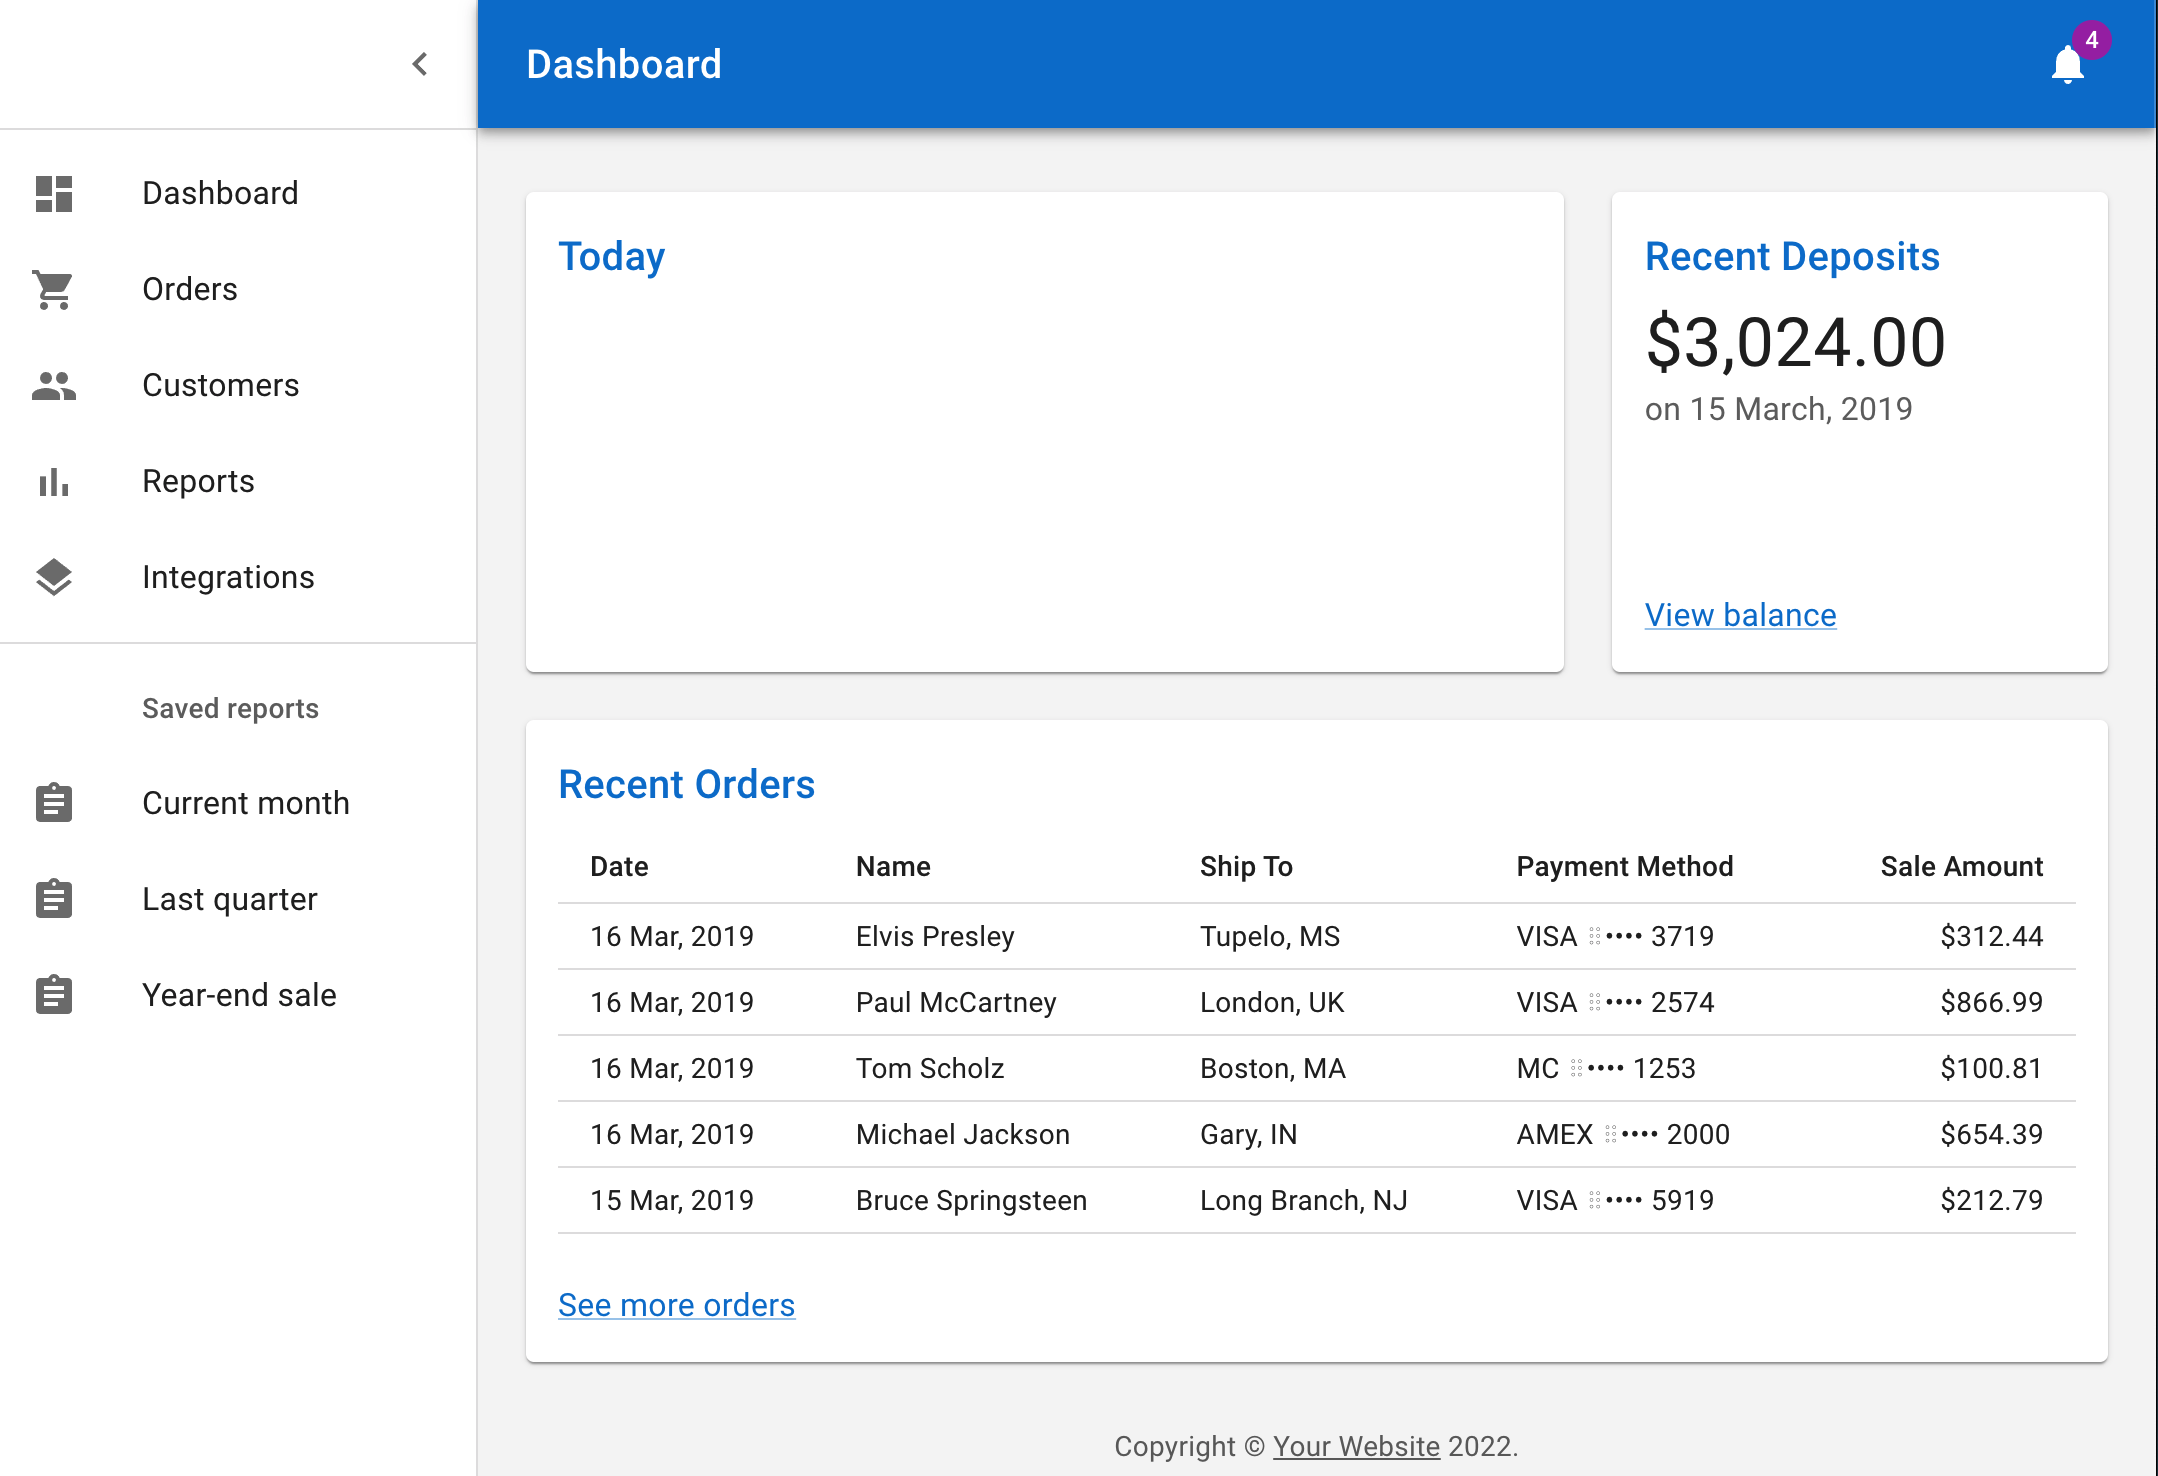
\includegraphics[width=0.5\maxwidth]{./images/03-todo-with-react/mui-sample.png}%
}%
\reviewimagecaption{MUIサンプル}
\label{image:03-todo-with-react:mui-sample}
\end{reviewimage}

もちろんカスタマイズも自由自在で、コンポーネントの各ページにあるサンプル付属のコードを
ブラウザ上でフロントエンド環境を試せる
CodeSandbox\footnote{\url{https://codesandbox.io/}}をクリック一発で開き、カスタマイズを試すことができます。

\begin{reviewimage}%%mui001-mui_compo_sample
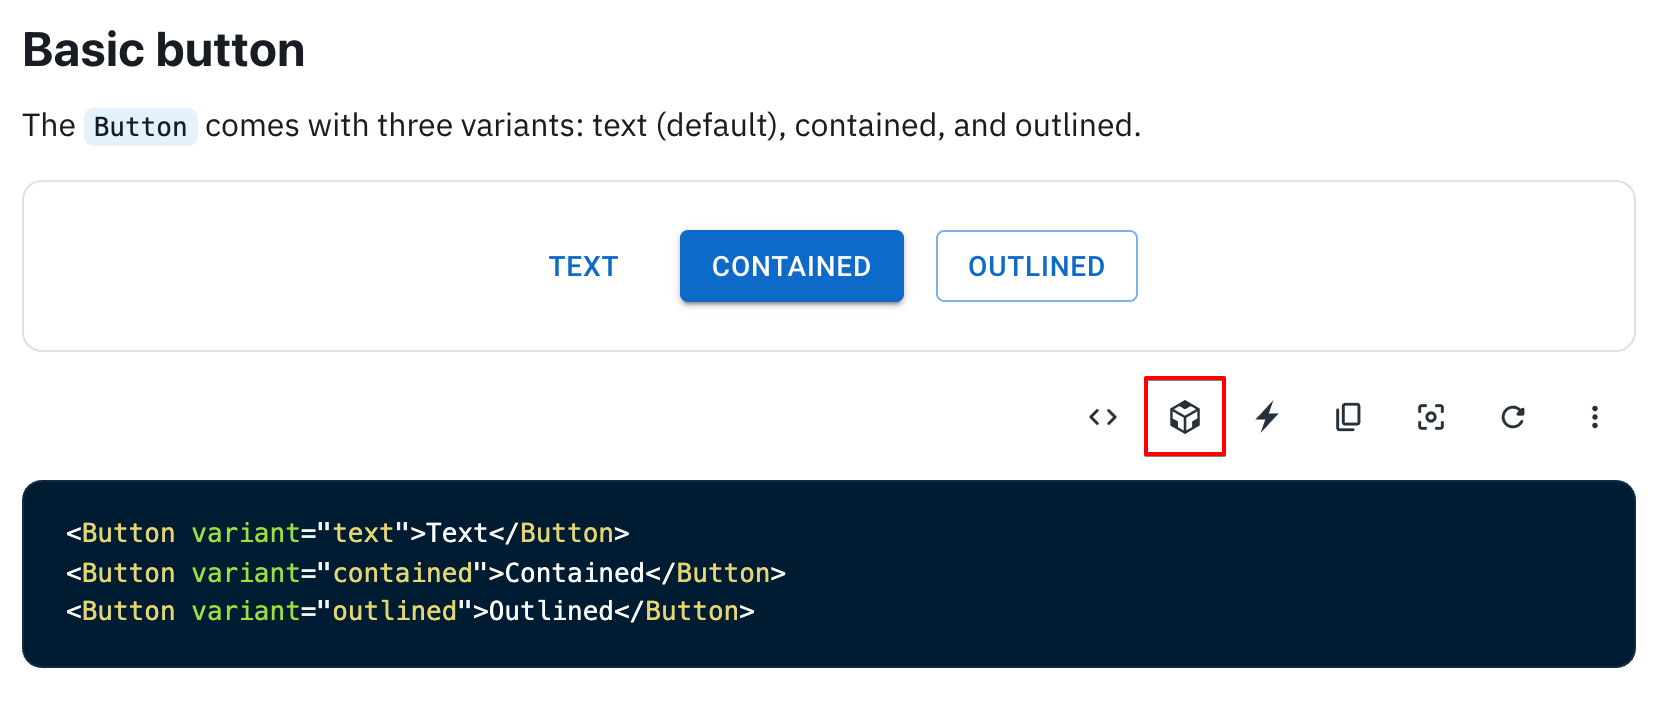
\includegraphics[width=0.6\maxwidth]{./images/03-todo-with-react/mui001-mui_compo_sample.png}%
\reviewimagecaption{コンポーネントのサンプル}
\label{image:03-todo-with-react:mui001-mui_compo_sample}
\end{reviewimage}
\begin{reviewimage}%%mui002-codesandbox
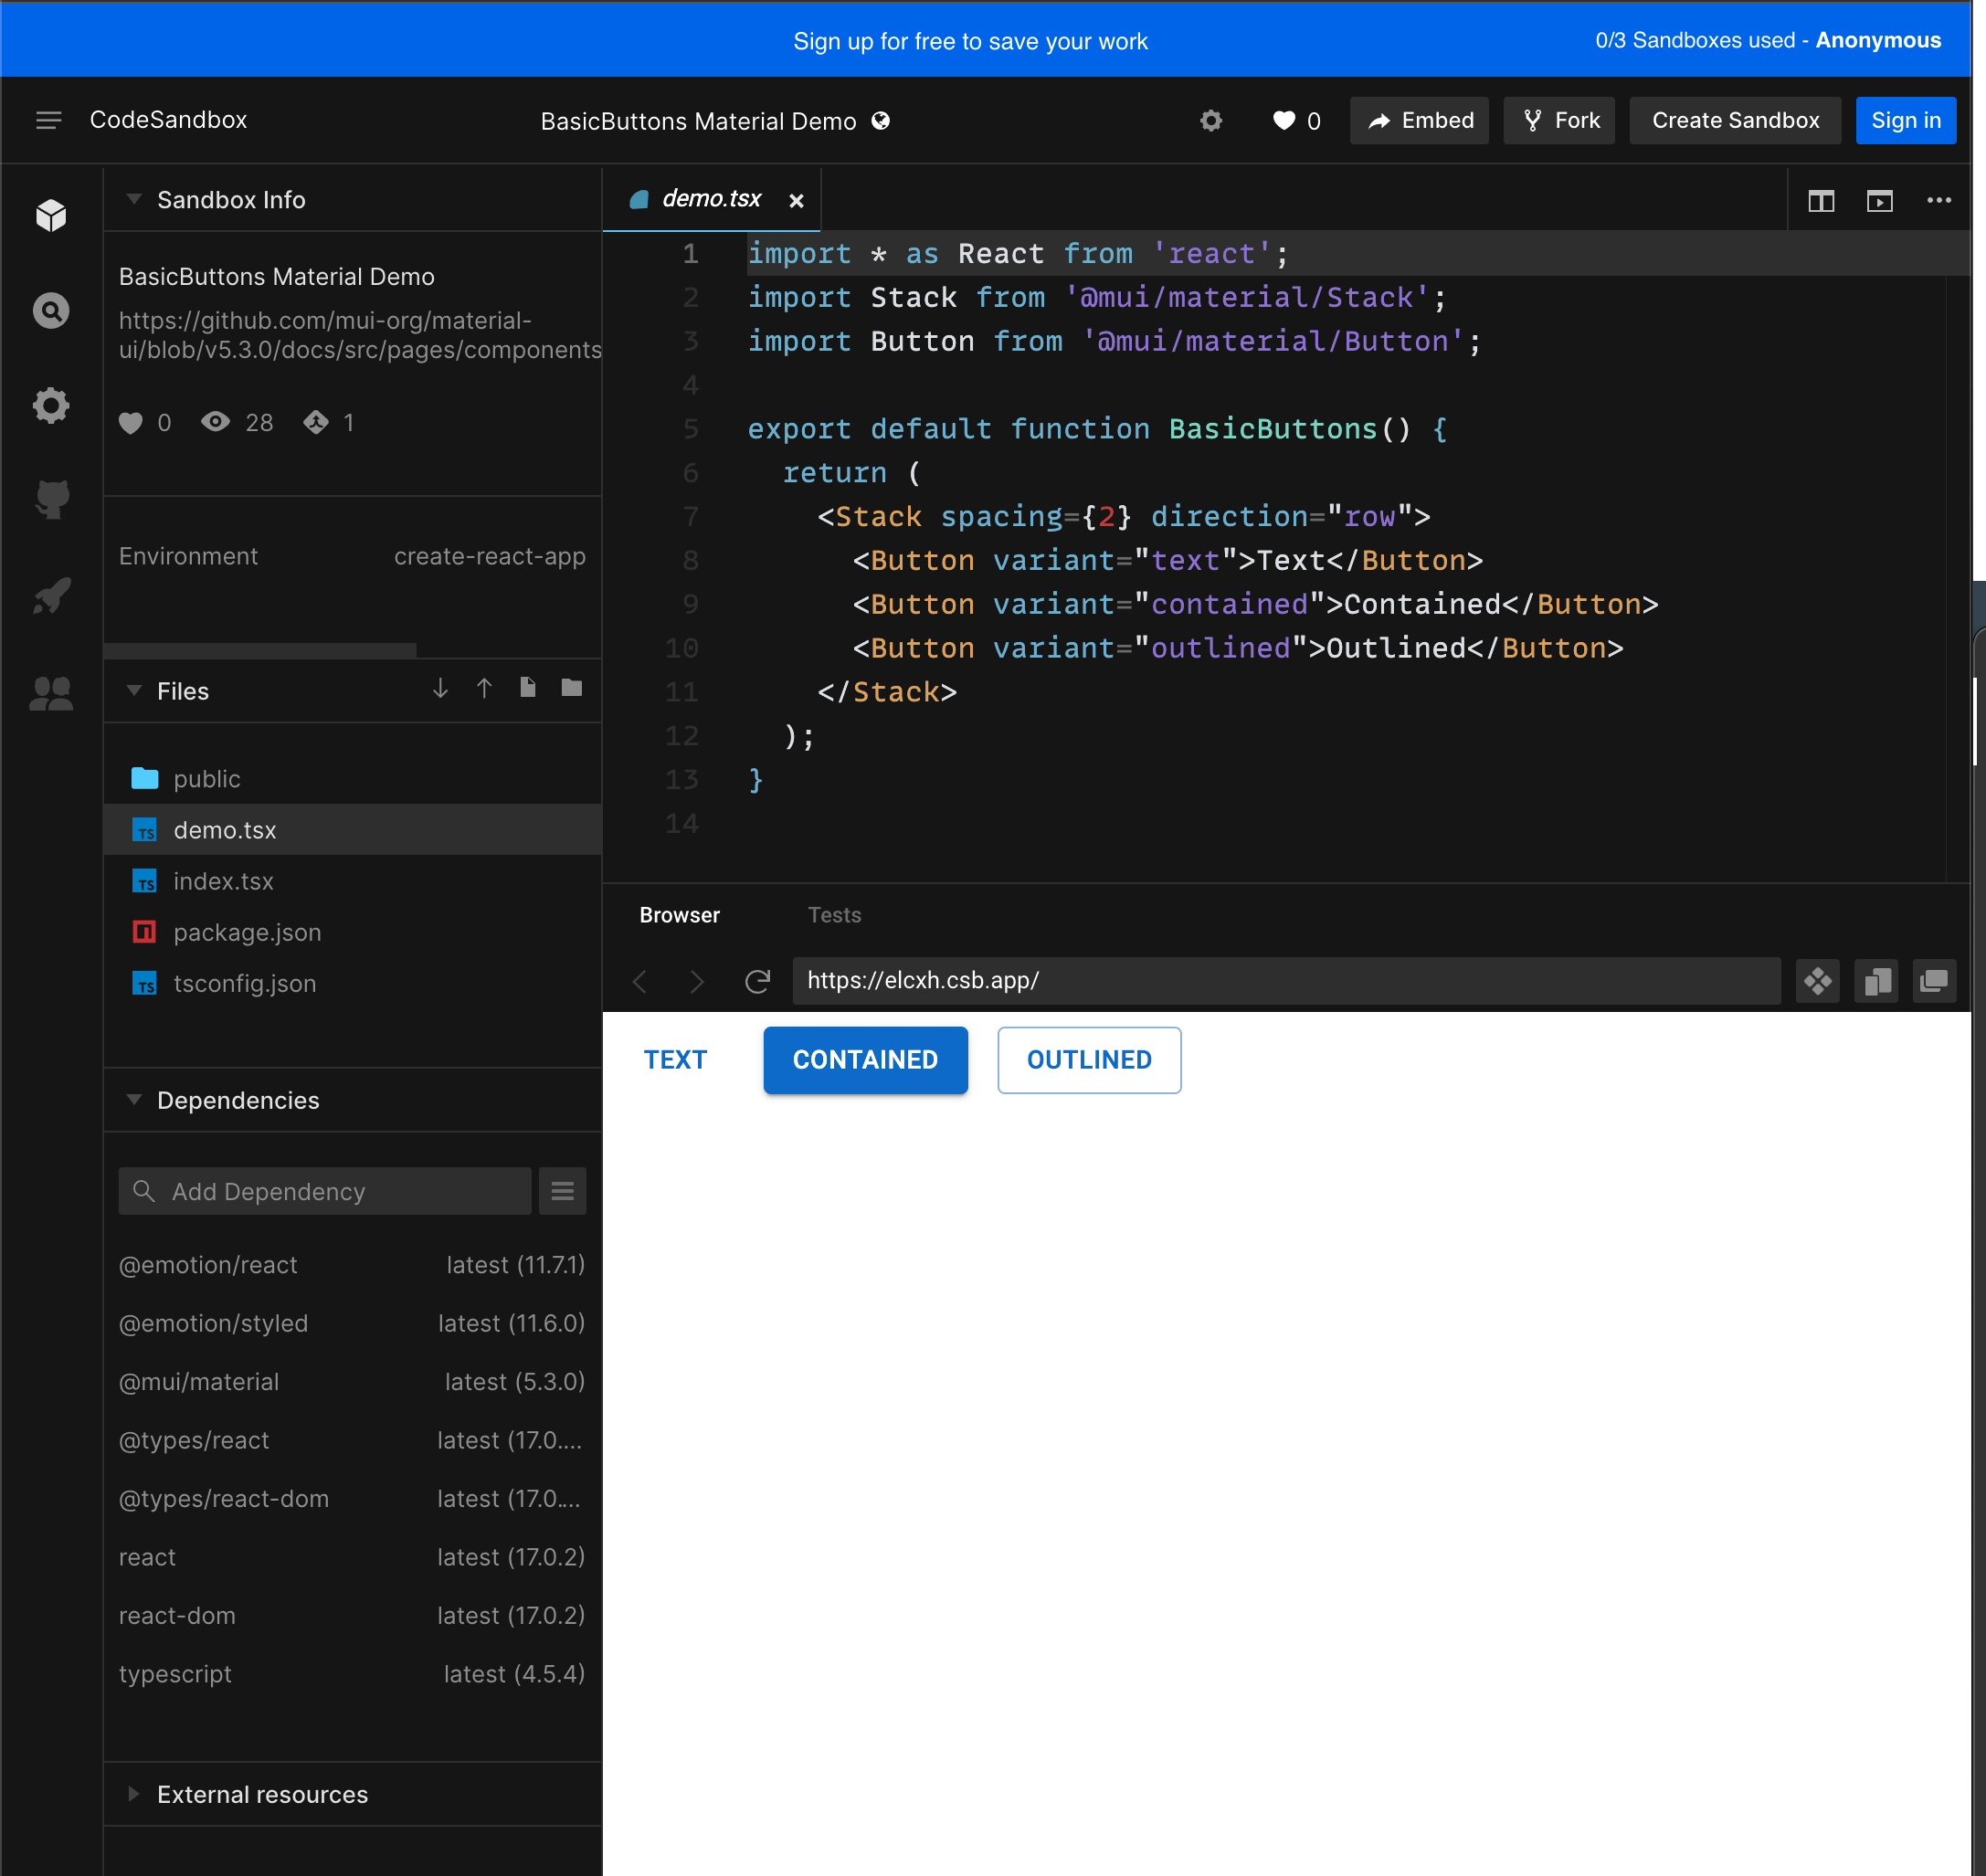
\includegraphics[width=0.6\maxwidth]{./images/03-todo-with-react/mui002-codesandbox.png}%
\reviewimagecaption{クリックでCodeSandboxを開いたところ}
\label{image:03-todo-with-react:mui002-codesandbox}
\end{reviewimage}

\subsection{MUIのインストール}
\keeplastskip{
  \label{sec:3-3-1}
  \label{sec-0330Install}
  \par\nobreak
}

MUIのインストールは、MUIトップページから「Get started」ボタンをクリックすると表示されます。

\begin{reviewimage}%%mui000-mui-top
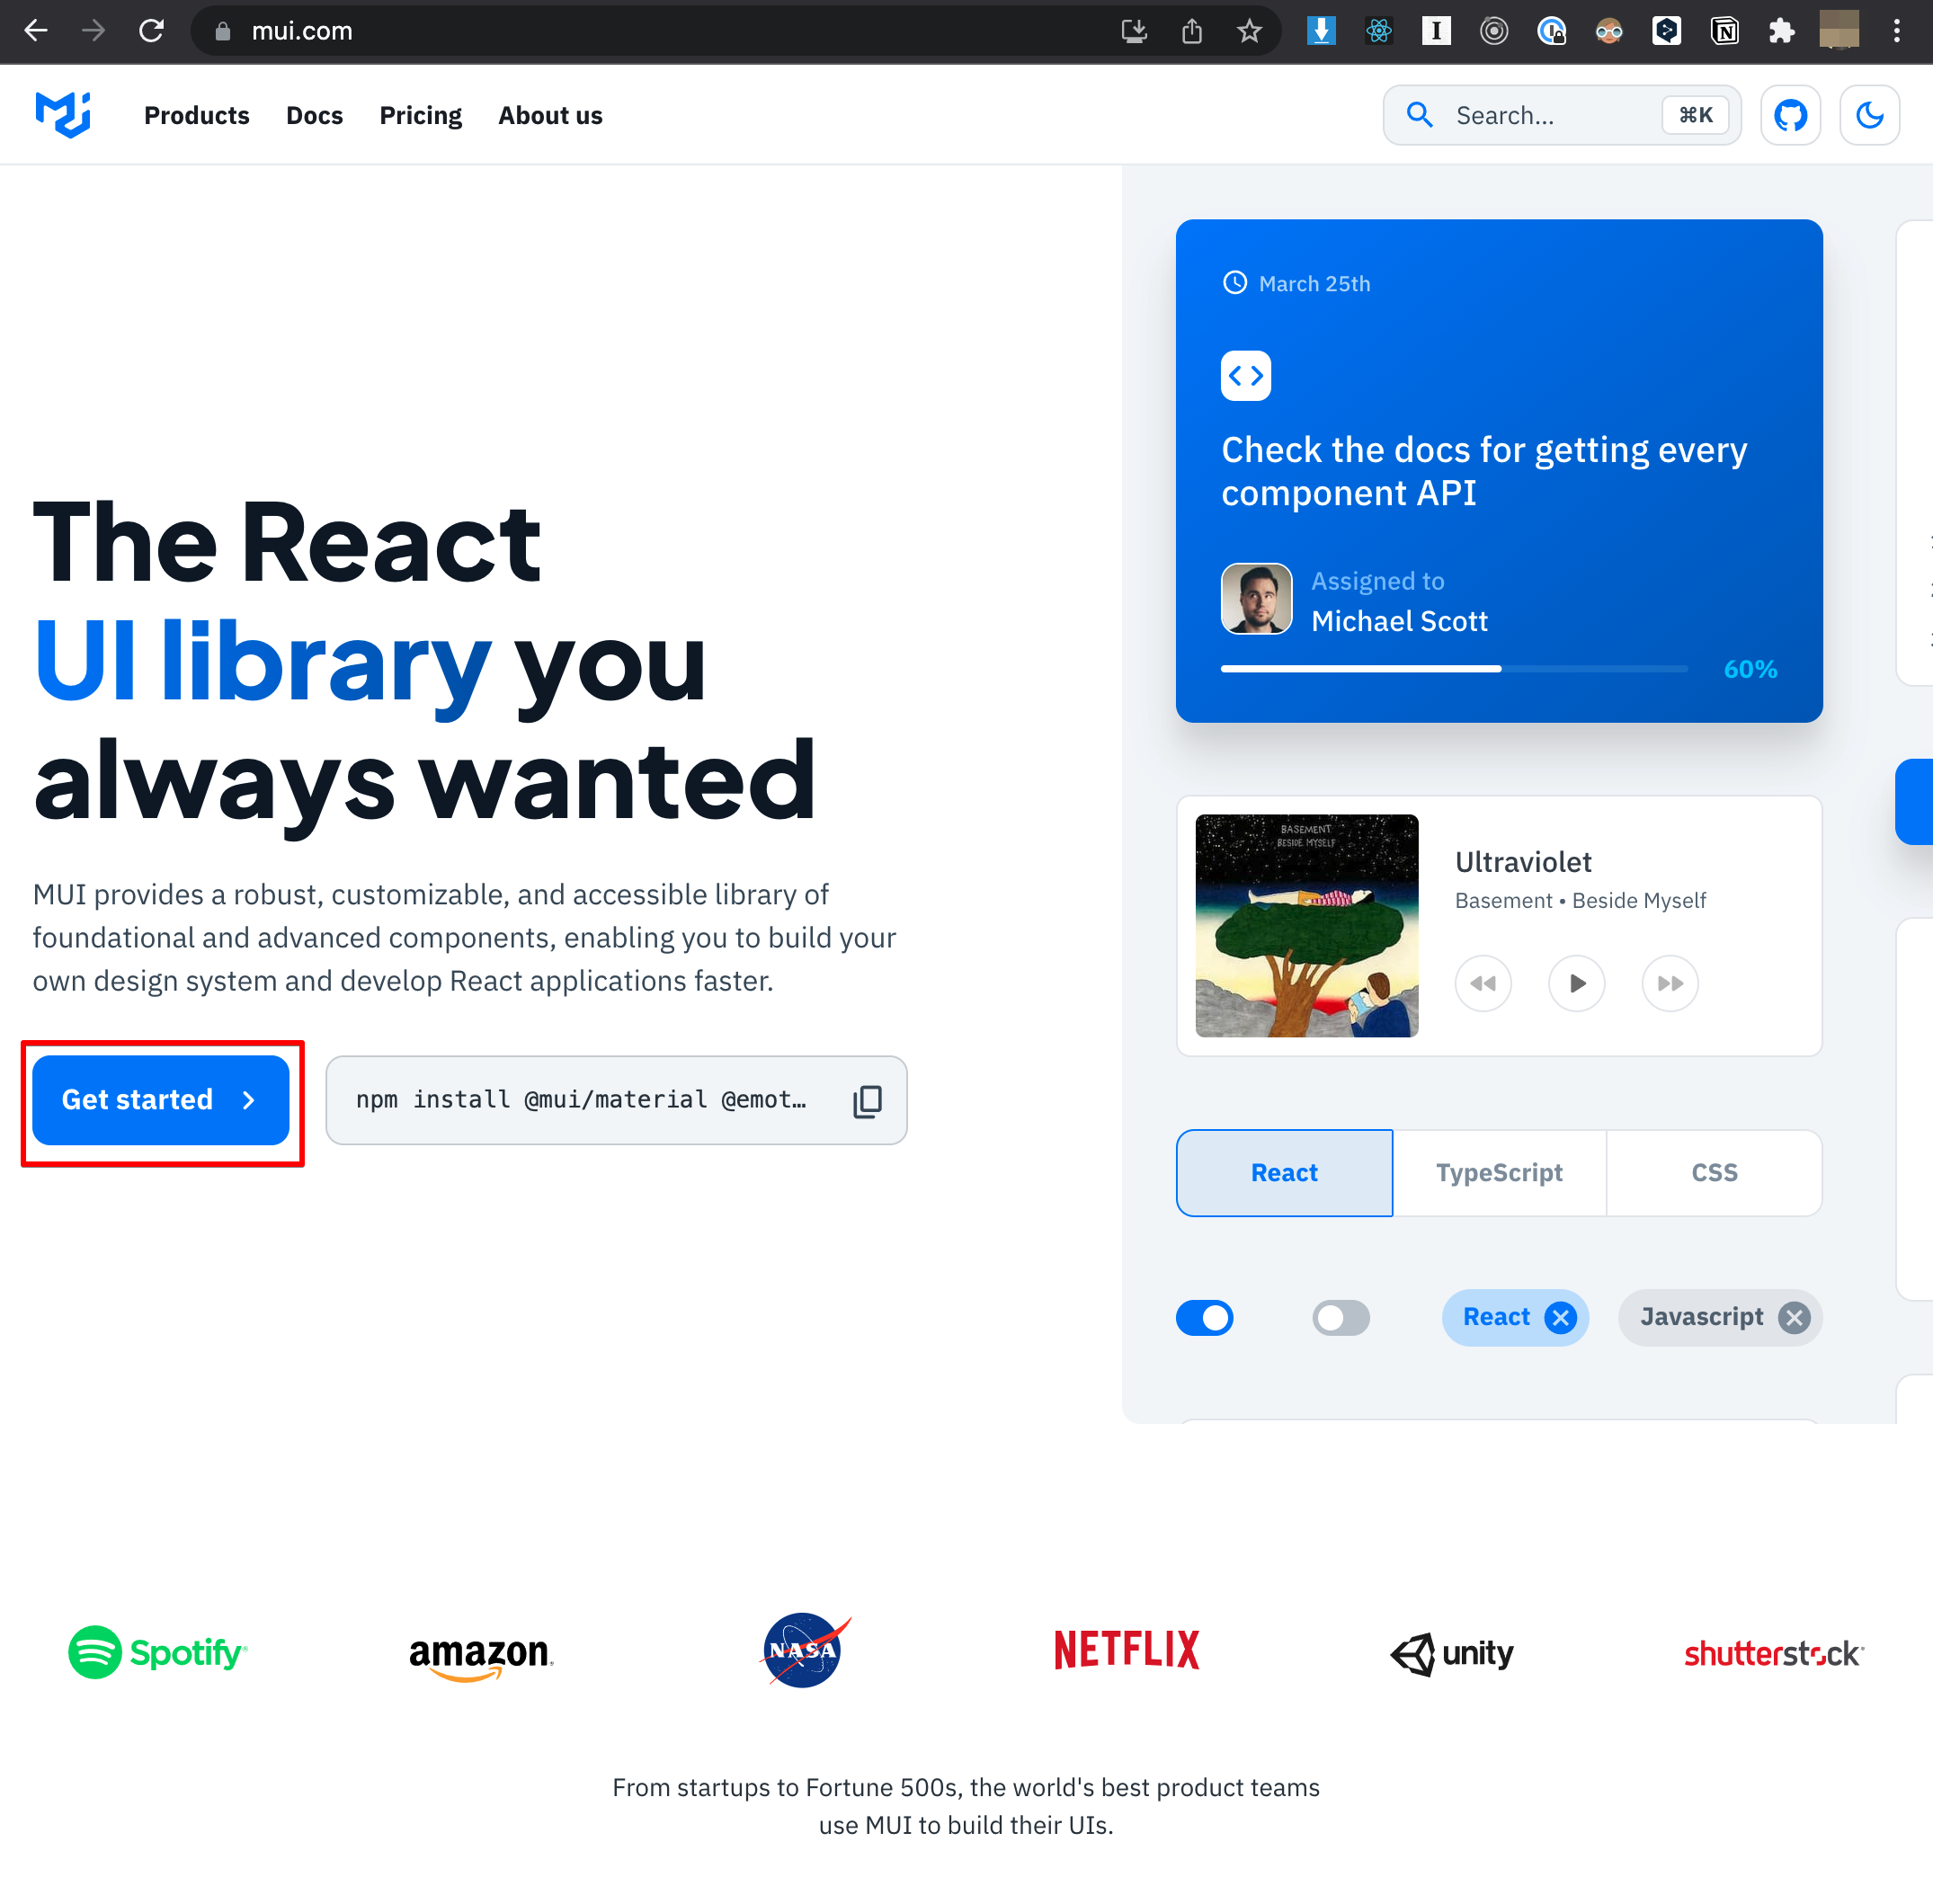
\includegraphics[width=0.5\maxwidth]{./images/03-todo-with-react/mui000-mui-top.png}%
\reviewimagecaption{MUIトップページ}
\label{image:03-todo-with-react:mui000-mui-top}
\end{reviewimage}

npmを使ったインストールは、material{-}iconも含め以下となります。

\def\startercodeblockfontsize{}
\begin{starterterminal}[]{MUIのインストール}\seqsplit{  \textgreater{} npm install @mui/material @emotion/react @emotion/styled @mui/icons{-}material}\end{starterterminal}
\begin{starternote}[]{}

ここまでの内容は、GitHub上で、以下のコマンドでクローンできます。

\def\startercodeblockfontsize{}
\begin{starterterminal}[]{GitHub}\seqsplit{\textgreater{} git clone {-}b 01\textunderscore{}install{-}MUI https://github.com/yaruo{-}react{-}redux/yaruo{-}diary.git}\end{starterterminal}
\end{starternote}

\subsection{データ表示画面を作る}
\keeplastskip{
  \label{sec:3-3-2}
  \label{sec-0330UI}
  \par\nobreak
}

データの一覧画面を作成します。

\vspace*{\baselineskip}

製品版の場合は、1画面に表示するデータ数を決め、それを超えた場合にはページネーションを作成しますが、
今回のサンプルアプリケーションは、1画面とします。

\vspace*{\baselineskip}

1画面のデータ表示を4とかに決め、ページネーションにて前後ページに移動するように魔改造してみてください。

\vspace*{\baselineskip}

では、データ表示コンポーネント(DiaryBoard)を作成します。
「/src/components」に「DiaryBoard.tsx」ファイルを作成します。

\subsection{MUI5のサイトからテンプレートを拝借}
\keeplastskip{
  \label{sec:3-3-3}
  \label{sec-0331}
  \par\nobreak
}

MUI5のサイトの左上部のメニューには、

\begin{starteritemize}
\item Getting Started

\begin{starteritemize}
\item Templates
\end{starteritemize}

\item Components

\begin{starteritemize}
\item Buttonなどのコンポーネント
\end{starteritemize}

\item Compotent API

\begin{starteritemize}
\item ComponentのProps(引数)の詳細
\end{starteritemize}

\end{starteritemize}

があります。

そのTemplateを選択すると、以下のようにMUIで作成されたサンプルページ(コンポーネントを組み合わせたもの)が表示されます。

\begin{reviewimage}%%mui004-templates
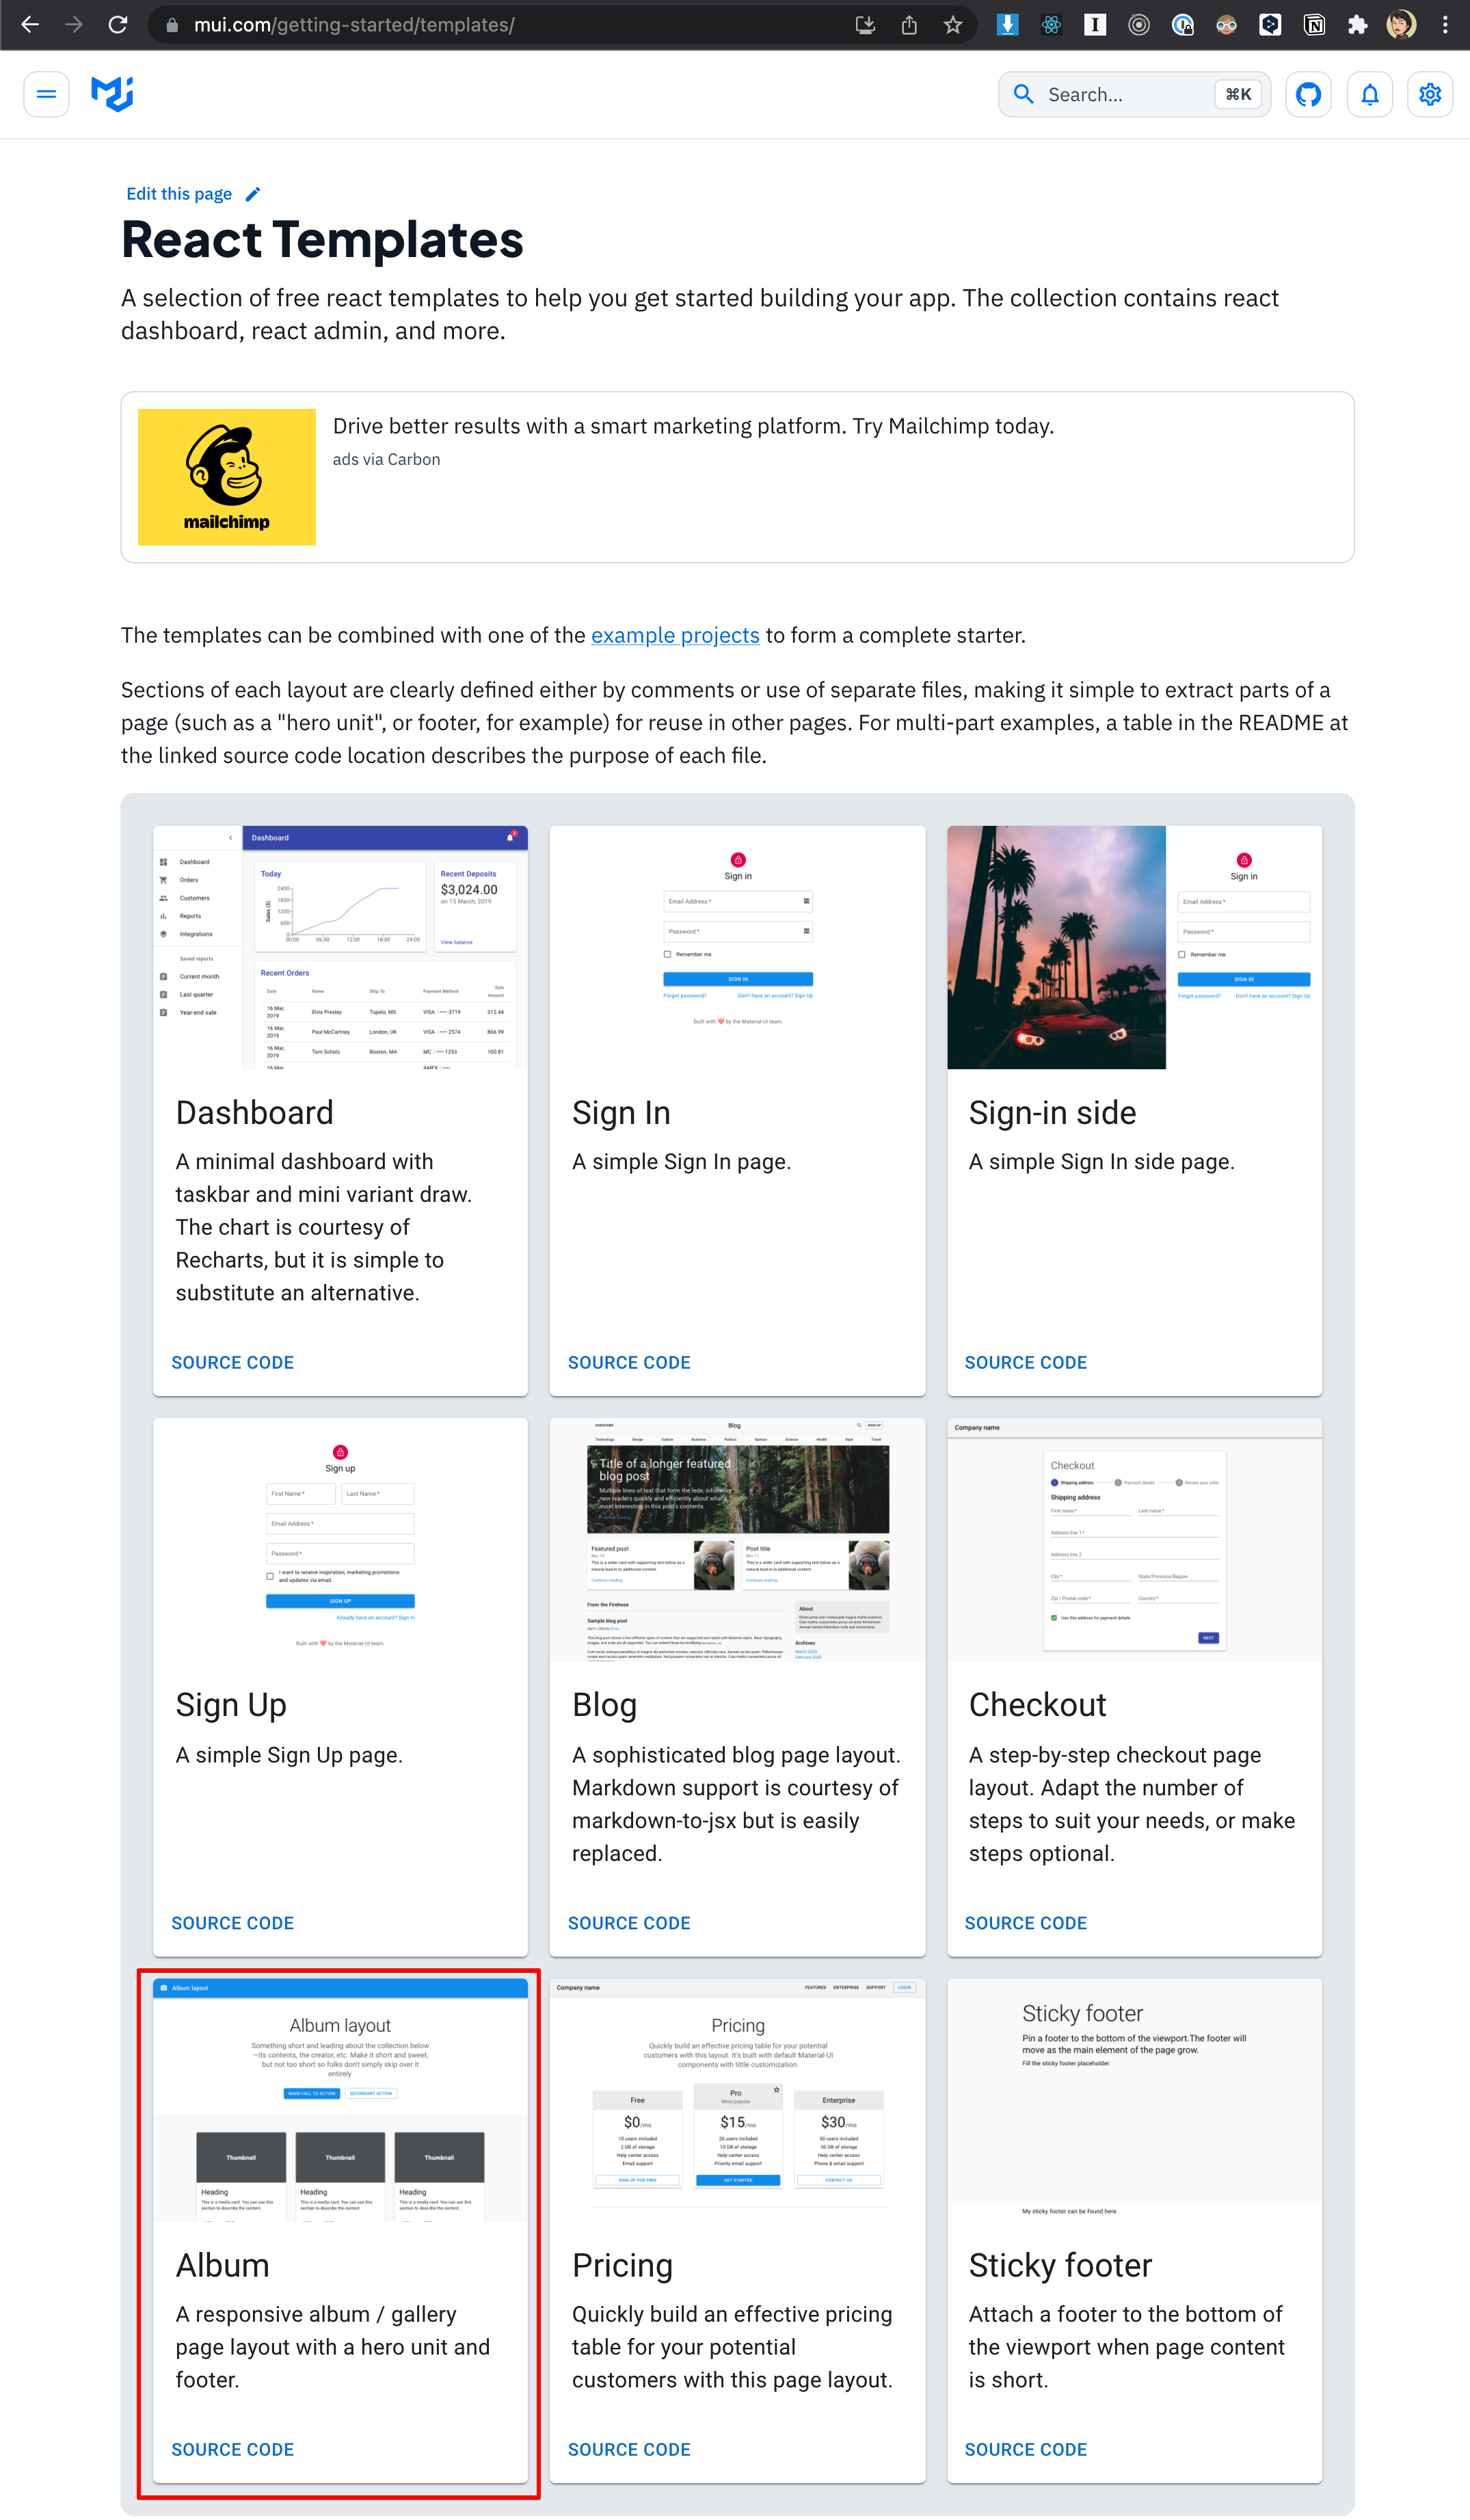
\includegraphics[width=0.5\maxwidth]{./images/03-todo-with-react/mui004-templates.png}%
\reviewimagecaption{MUIのTemplateページ}
\label{image:03-todo-with-react:mui004-templates}
\end{reviewimage}

今回は、この中から「Album layout」を拝借して改造していきます。


\clearpage

\begin{reviewimage}%%mui005-albumLayout
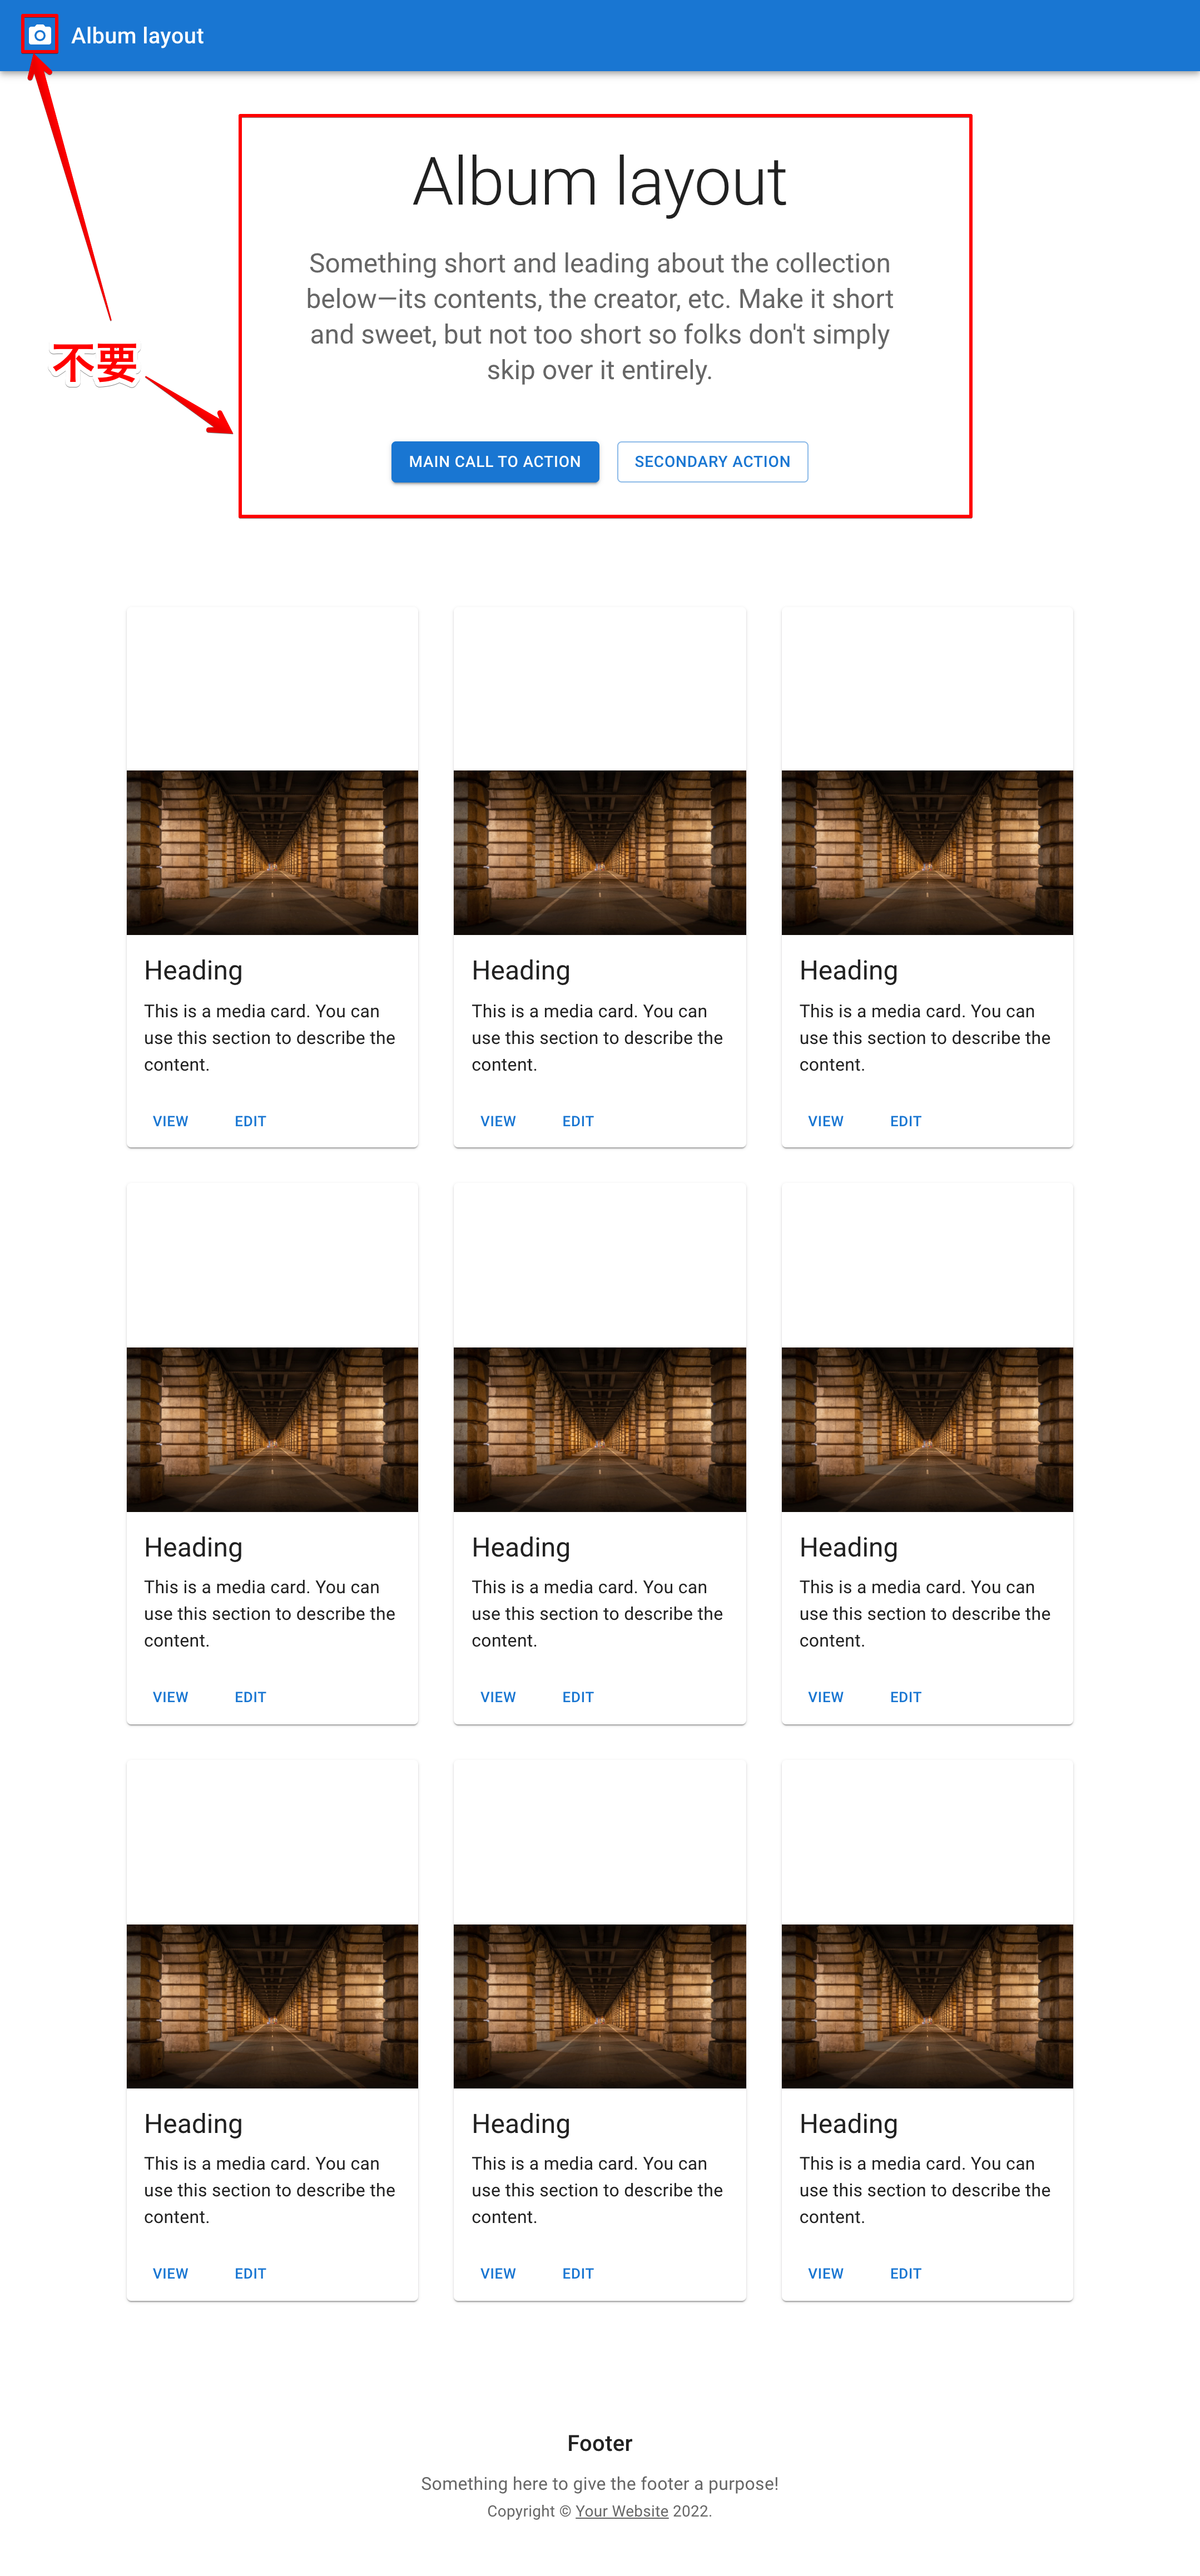
\includegraphics[width=0.5\maxwidth]{./images/03-todo-with-react/mui005-albumLayout.png}%
\reviewimagecaption{アルバムレイアウト}
\label{image:03-todo-with-react:mui005-albumLayout}
\end{reviewimage}

先ほどのテンプレートページの「Album Layout」内の「SOURCECODE」をクリックします。


\clearpage

\begin{reviewimage}%%mui006-albumLayoutSource
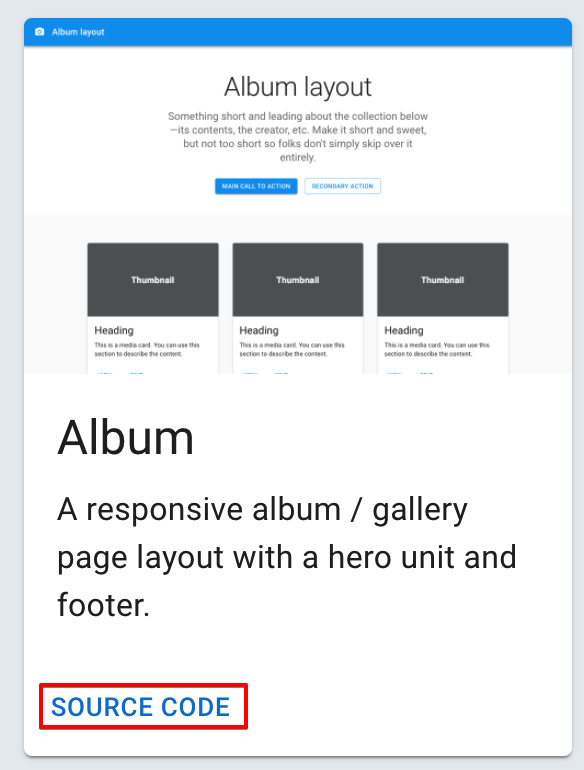
\includegraphics[width=0.4\maxwidth]{./images/03-todo-with-react/mui006-albumLayoutSource.png}%
\reviewimagecaption{ソースコードへのリンク}
\label{image:03-todo-with-react:mui006-albumLayoutSource}
\end{reviewimage}

MUIのGitHubが開き、JavaScript、TypeScriptのソースコードがあります。今回は、Album.tsxを開きます。

\begin{reviewimage}%%mui007-albumLayoutSourceCode
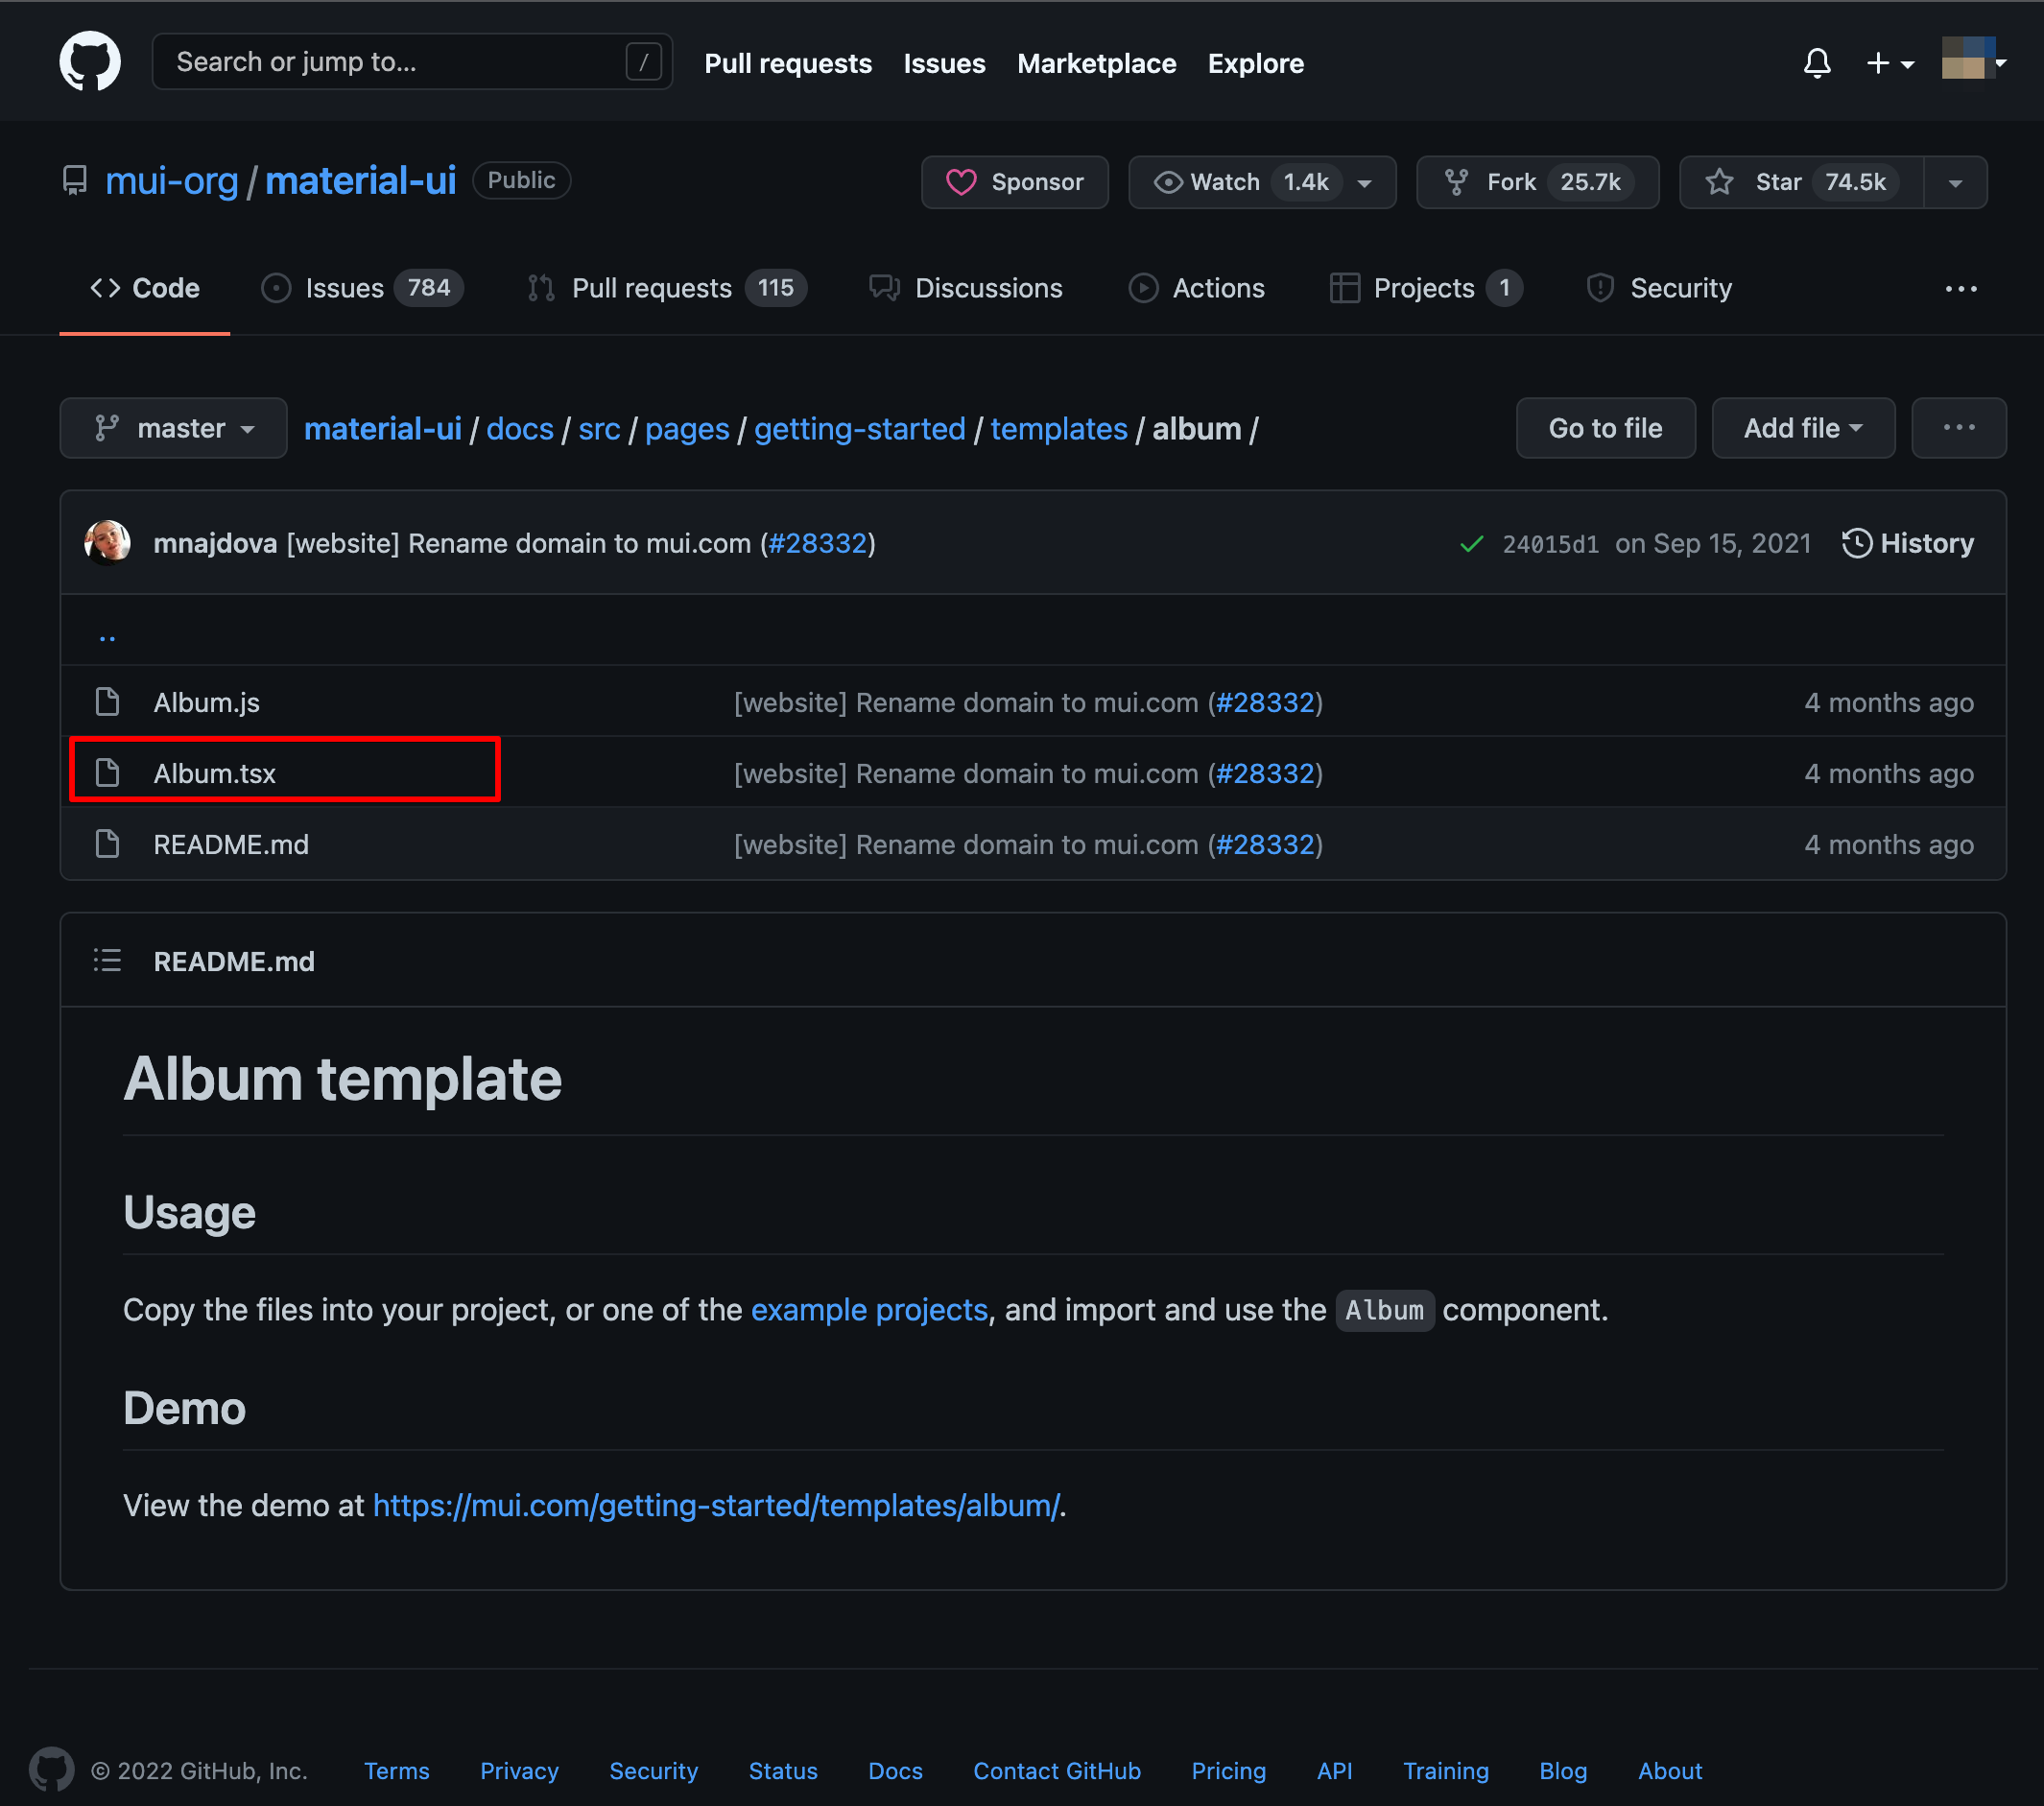
\includegraphics[width=0.6\maxwidth]{./images/03-todo-with-react/mui007-albumLayoutSourceCode.png}%
\reviewimagecaption{GitHubでのAlbumのソースコード}
\label{image:03-todo-with-react:mui007-albumLayoutSourceCode}
\end{reviewimage}

\clearpage


このコードを作成した「DiaryBoard.tsx」ファイルへ貼り付け、以下を変更します。

\begin{starteritemize}
\item コンポーネント名(関数名)を「DiaryBoard」へ。
\item ThemeProviderコンポーネント、CssBaselineコンポーネントを削除。
\item ThemeProviderコンポーネントの位置に、\textless{}\textgreater{}\textless{}/\textgreater{}を置くこと。
\item Hero unit、カメラアイコンの削除。
\item 「const theme = createTheme()」を削除。
\item functionをアロー関数に変更。
\item 削除したコンポーネントのimport文を削除。
\end{starteritemize}

「\textless{}\textgreater{}\textless{}/\textgreater{}」をトップのタグにした理由は、「Jsxはひとつの要素のみ」と怒られるからです。
このタグをトップに置くことで、要素は1つ(ほかは子要素)となります。また、不要なdivタグに変換されません。

\vspace*{\baselineskip}

変更の完了したコードがこちらです。なります。

\def\startercodeblockfontsize{}
\begin{starterprogram}[]{src/components/DiaryBoard.tsx}\seqsplit{  import * as React from 'react';
  import AppBar from '@mui/material/AppBar';
  import Button from '@mui/material/Button';
  import Card from '@mui/material/Card';
  import CardActions from '@mui/material/CardActions';
  import CardContent from '@mui/material/CardContent';
  import CardMedia from '@mui/material/CardMedia';
  import Grid from '@mui/material/Grid';
  import Box from '@mui/material/Box';
  import Toolbar from '@mui/material/Toolbar';
  import Typography from '@mui/material/Typography';
  import Container from '@mui/material/Container';
  import Link from '@mui/material/Link';

  const Copyright = () =\textgreater{} (
    \textless{}Typography variant='body2' color='text.secondary' align='center'\textgreater{}
      \{'Copyright © '\}
      \textless{}Link color='inherit' href='https://mui.com/'\textgreater{}
        Your Website
      \textless{}/Link\textgreater{}
      \{` \textdollar{}\{new Date().getFullYear()\}.`\}
    \textless{}/Typography\textgreater{}
  );

  const cards = [1, 2, 3, 4, 5, 6, 7, 8, 9];

  const DiaryBoard = () =\textgreater{} (
    \textless{}\textgreater{}
      \textless{}AppBar position='relative'\textgreater{}
        \textless{}Toolbar\textgreater{}
          \textless{}Typography variant='h6' color='inherit' noWrap\textgreater{}
            やる夫の読書日記
          \textless{}/Typography\textgreater{}
        \textless{}/Toolbar\textgreater{}
      \textless{}/AppBar\textgreater{}
      \textless{}main\textgreater{}
        \textless{}Container sx=\{\{ py: 8 \}\} maxWidth='md'\textgreater{}
          \textless{}Grid container spacing=\{4\}\textgreater{}
            \{cards.map((card) =\textgreater{} (
              \textless{}Grid item key=\{card\} xs=\{12\} sm=\{6\} md=\{4\}\textgreater{}
                \textless{}Card
                  sx=\{\{
                    height: '100\%',
                    display: 'flex',
                    flexDirection: 'column',
                  \}\}
                \textgreater{}
                  \textless{}CardMedia
                    component='img'
                    sx=\{\{
                      // 16:9
                      pt: '56.25\%',
                    \}\}
                    image='https://source.unsplash.com/random'
                    alt='random'
                  /\textgreater{}
                  \textless{}CardContent sx=\{\{ flexGrow: 1 \}\}\textgreater{}
                    \textless{}Typography gutterBottom variant='h5' component='h2'\textgreater{}
                      Heading
                    \textless{}/Typography\textgreater{}
                    \textless{}Typography\textgreater{}
                      This is a media card. You can use this section to describe
                      the content.
                    \textless{}/Typography\textgreater{}
                  \textless{}/CardContent\textgreater{}
                  \textless{}CardActions\textgreater{}
                    \textless{}Button size='small'\textgreater{}View\textless{}/Button\textgreater{}
                    \textless{}Button size='small'\textgreater{}Edit\textless{}/Button\textgreater{}
                  \textless{}/CardActions\textgreater{}
                \textless{}/Card\textgreater{}
              \textless{}/Grid\textgreater{}
            ))\}
          \textless{}/Grid\textgreater{}
        \textless{}/Container\textgreater{}
      \textless{}/main\textgreater{}
      \{/* Footer */\}
      \textless{}Box sx=\{\{ bgcolor: 'background.paper', p: 6 \}\} component='footer'\textgreater{}
        \textless{}Typography variant='h6' align='center' gutterBottom\textgreater{}
          Footer
        \textless{}/Typography\textgreater{}
        \textless{}Typography
          variant='subtitle1'
          align='center'
          color='text.secondary'
          component='p'
        \textgreater{}
          Something here to give the footer a purpose!
        \textless{}/Typography\textgreater{}
        \textless{}Copyright /\textgreater{}
      \textless{}/Box\textgreater{}
      \{/* End footer */\}
    \textless{}/\textgreater{}
  );

  export default DiaryBoard;
}\end{starterprogram}

次に、Appコンポーネントを変更し、DiaryBoardコンポーネントを表示するように変更します。
また、先ほど削除した「ThemeProvider」、「CssBaseline」、「createTheme()」も追加します。

追加完了したコードが以下となります。

\def\startercodeblockfontsize{}
\begin{starterprogram}[]{変更後のAppコンポーネント}\seqsplit{  import React from 'react';
  import CssBaseline from '@mui/material/CssBaseline';
  import \{ createTheme, ThemeProvider \} from '@mui/material/styles';

  import DiaryBoard from './DiaryBoard';

  const theme = createTheme();

  const App = () =\textgreater{} (
    \textless{}ThemeProvider theme=\{theme\}\textgreater{}
      \textless{}CssBaseline /\textgreater{}
      \textless{}DiaryBoard /\textgreater{}
    \textless{}/ThemeProvider\textgreater{}
  );

  export default App;}\end{starterprogram}

最後に、不要になった「style.css」、「style.scss」を削除し、「index.tsx」を変更します。

\def\startercodeblockfontsize{}
\begin{starterprogram}[]{index.tsx}\seqsplit{  import React from 'react';
  import ReactDOM from 'react{-}dom';
  import App from './components/App';

  ReactDOM.render(
    \textless{}div\textgreater{}
      \textless{}App /\textgreater{}
    \textless{}/div\textgreater{},
    document.getElementById('root')
  );}\end{starterprogram}

以上の変更が完了しましたら、動作確認します。

\def\startercodeblockfontsize{}
\begin{starterterminal}[]{サンプルアプリケーションの動作確認}\seqsplit{  \textgreater{} npm run start}\end{starterterminal}

この画面が表示されれば正常です。カードの画像はランダムですので、違っていてもかまいません。

\begin{reviewimage}%%mui008-album-done
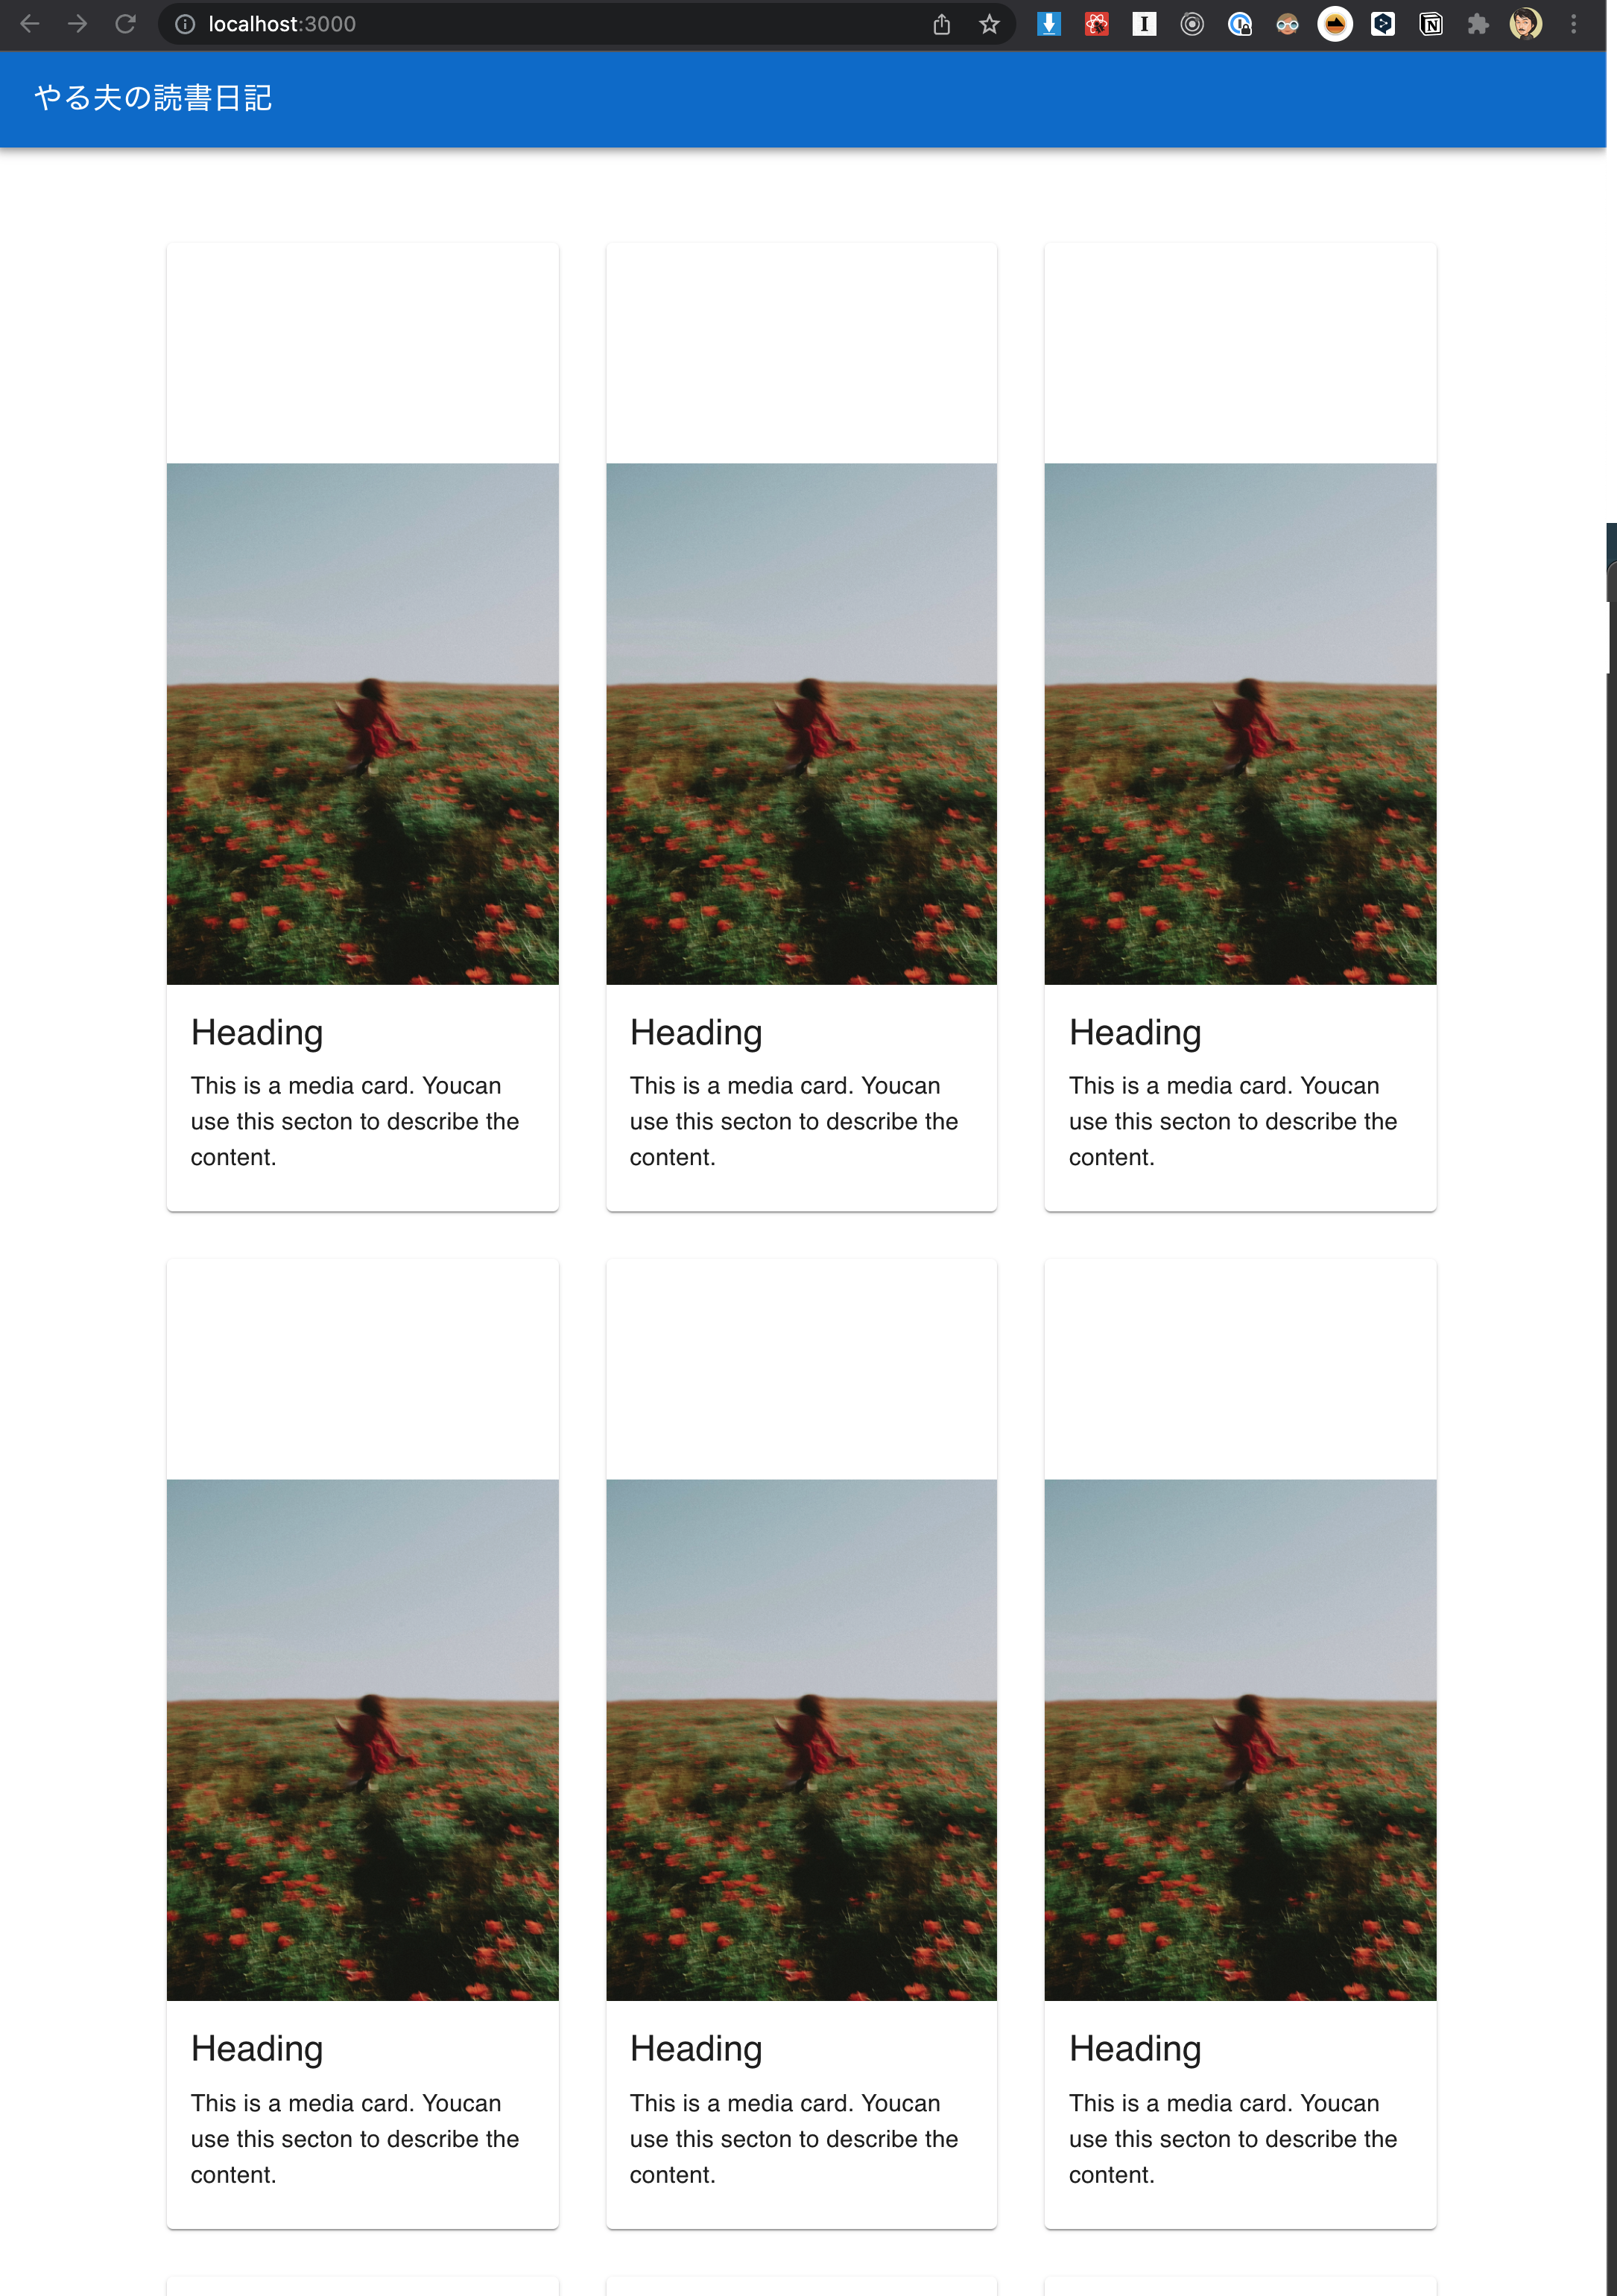
\includegraphics[width=0.8\maxwidth]{./images/03-todo-with-react/mui008-album-done.png}%
\reviewimagecaption{Album Layoutの拝借}
\label{image:03-todo-with-react:mui008-album-done}
\end{reviewimage}

\clearpage


\subsection{カード一覧画面の表示}
\keeplastskip{
  \label{sec:3-3-4}
  \label{sec-0332}
  \par\nobreak
}

カード表示用のボードができましたので、表示するカードは別なものにしましょう。

\vspace*{\baselineskip}

MUIのメニューから「Components \textgreater{} Card」をクリックすると、たくさんのサンプルがあります。
少し下へスクロールすると、こちらが見つかりました。
「\textless{}\textgreater{}」アイコンをクリックすると、JS/TS別にソースコードが憑依されます。

\begin{reviewimage}%%mui009-card-ComplexInteraction
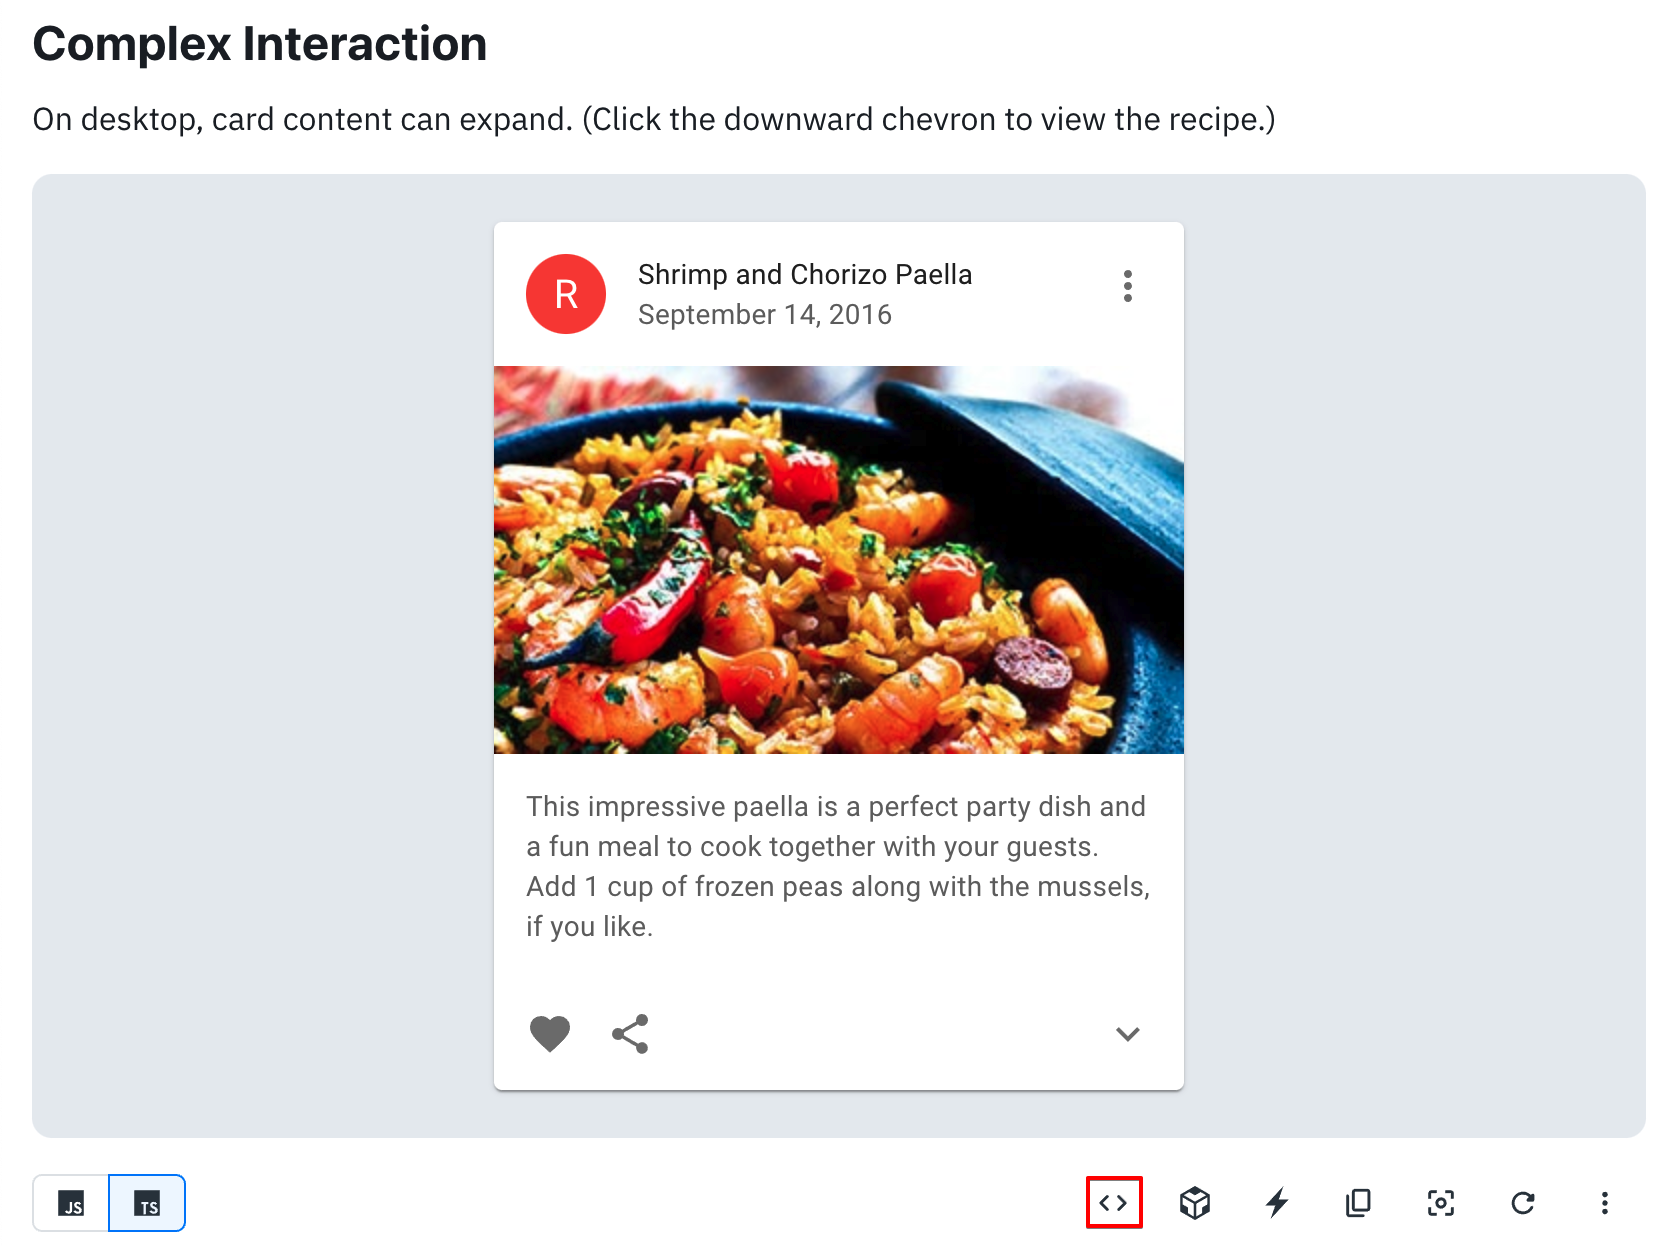
\includegraphics[width=1.0\maxwidth]{./images/03-todo-with-react/mui009-card-ComplexInteraction.png}%
\reviewimagecaption{MUIカードサンプル}
\label{image:03-todo-with-react:mui009-card-ComplexInteraction}
\end{reviewimage}

「src/components/」フォルダに「DiaryCard.tsx」ファイルを作成しソースコードをコピペします。

以下を変更します。

\begin{starteritemize}
\item 1行目「import * as React」を「import React」へ(理由はのちほど)
\item function関数をアロー関数へ
\item 関数名の変更「DiaryCard」へ
\item 表示するデータをProps(引数)として受け取る
\item 受け取ったオブジェクトを表示するようにtsxに埋め込む
\end{starteritemize}

\subsubsection*{import * as React呪文}
\keeplastskip{
  \label{sec:3-3-4-1}
  \label{sec-00332-1}
  \par\nobreak
}

「import」は、ES6仕様のモジュール読み込み方法です。

\vspace*{\baselineskip}

\begin{description}
\item[import * as React from 'react' の場合] \mbox{} \\
fromにある「react」がexportしているものすべてをインポート
\item[import React from 'react' の場合] \mbox{} \\
fromにある「react」が「default」でexportしているものだけをインポート
\end{description}

\vspace*{\baselineskip}

結果としての違いは、webpackでバンドルした場合に作成されるビルドファイルはインポートされたものを含むため、
使用しないものまでインポートするとファイルサイズが肥大化する恐れがあります。

\subsubsection*{function関数をアロー関数へ}
\keeplastskip{
  \label{sec:3-3-4-2}
  \label{sec-00332-2}
  \par\nobreak
}

ファンクション関数とアロー関数の違いについては、
こちらの記事\footnote{\url{https://qiita.com/suin/items/a44825d253d023e31e4d}}が参考になります。

\begin{reviewimage}%%sec00332-1-01
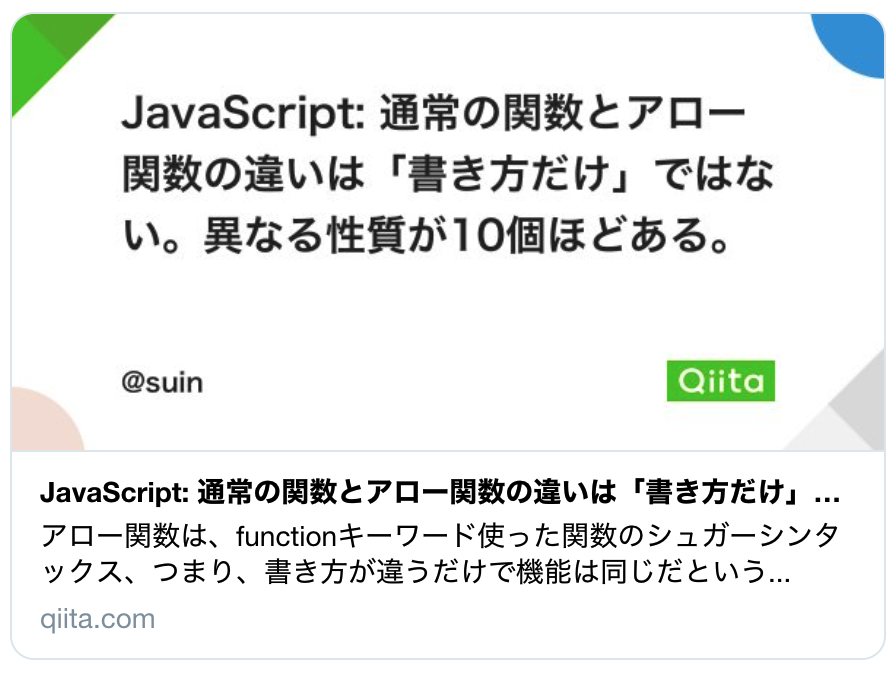
\includegraphics[width=0.5\maxwidth]{./images/03-todo-with-react/sec00332-1-01.png}%
\reviewimagecaption{ファンクション関数とアロー関数の違い}
\label{image:03-todo-with-react:sec00332-1-01}
\end{reviewimage}

また、Reactでアロー関数を使うことについては、
こちらの記事\footnote{\url{https://zenn.dev/seya/articles/0317b7a61ee781}}が参考になります。

\begin{reviewimage}%%sec00332-1-02
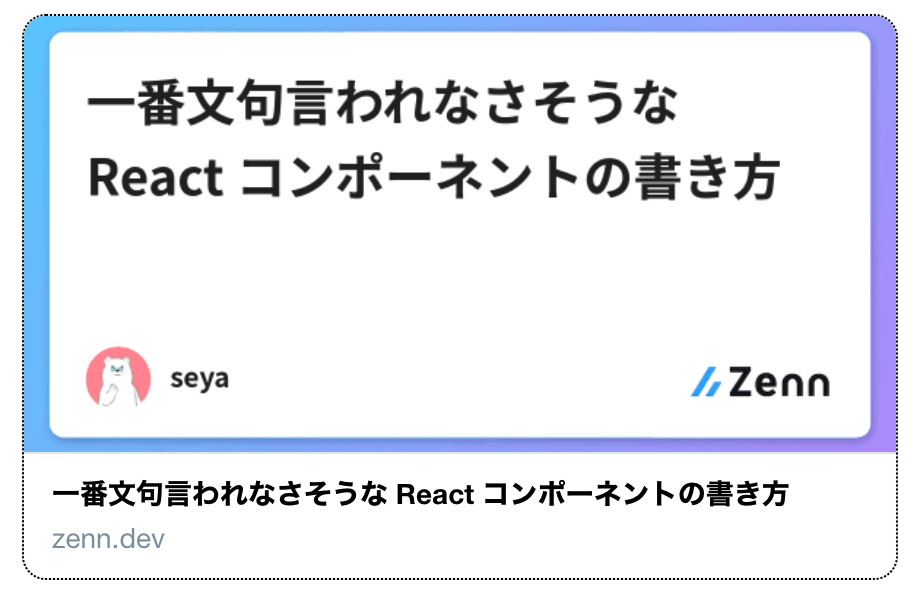
\includegraphics[width=0.5\maxwidth]{./images/03-todo-with-react/sec00332-1-02.png}%
\reviewimagecaption{Reactコンポーネントの書き方}
\label{image:03-todo-with-react:sec00332-1-02}
\end{reviewimage}

\subsubsection*{関数名の変更}
\keeplastskip{
  \label{sec:3-3-4-3}
  \label{sec-00332-3}
  \par\nobreak
}

関数名を「RecipeReviewCard」から「DiaryCard」へ変更します。
exportも忘れずに。

\subsubsection*{表示するデータを受け取る}
\keeplastskip{
  \label{sec:3-3-4-4}
  \label{sec-00332-4}
  \par\nobreak
}

Reactコンポーネントのjsx(tsx)では、HTML内にJavaScriptのオブジェクトを「\{\}」で埋め込み表示できます。

TypeScriptでは、受け取るオブジェクトの型を定義します。

\vspace*{\baselineskip}

コンポーネントは、表示するためのデータ(表示する子要素も含む)を「Props(プロパティの意味)」として受け取ります。
コンポーネント関数からしてみると引数にあたります。

受け取るProps(引数)の型を、「src/diaryData.ts」ファイルを作成し定義します。このファイルは、のちほど初期値も追加します。

\subsubsection*{受け取ったオブジェクトを埋め込む}
\keeplastskip{
  \label{sec:3-3-4-5}
  \label{sec-00332-5}
  \par\nobreak
}
\vspace*{\baselineskip}

受け取ったオブジェクトを変数に展開し、表示位置に埋め込みます。

\subsubsection*{DiaryCardを表示する}
\keeplastskip{
  \label{sec:3-3-4-6}
  \label{sec-00332-6}
  \par\nobreak
}

初期値を設定し、Appコンポーネントに「DiaryBoard」の代わりに表示してみます。こちらが表示されれば完成です。
もちろん、「下向き」をクリックすると詳細部分が表示されます。readmore配列の各要素が段落になっています。

\begin{reviewimage}%%sec00332-6
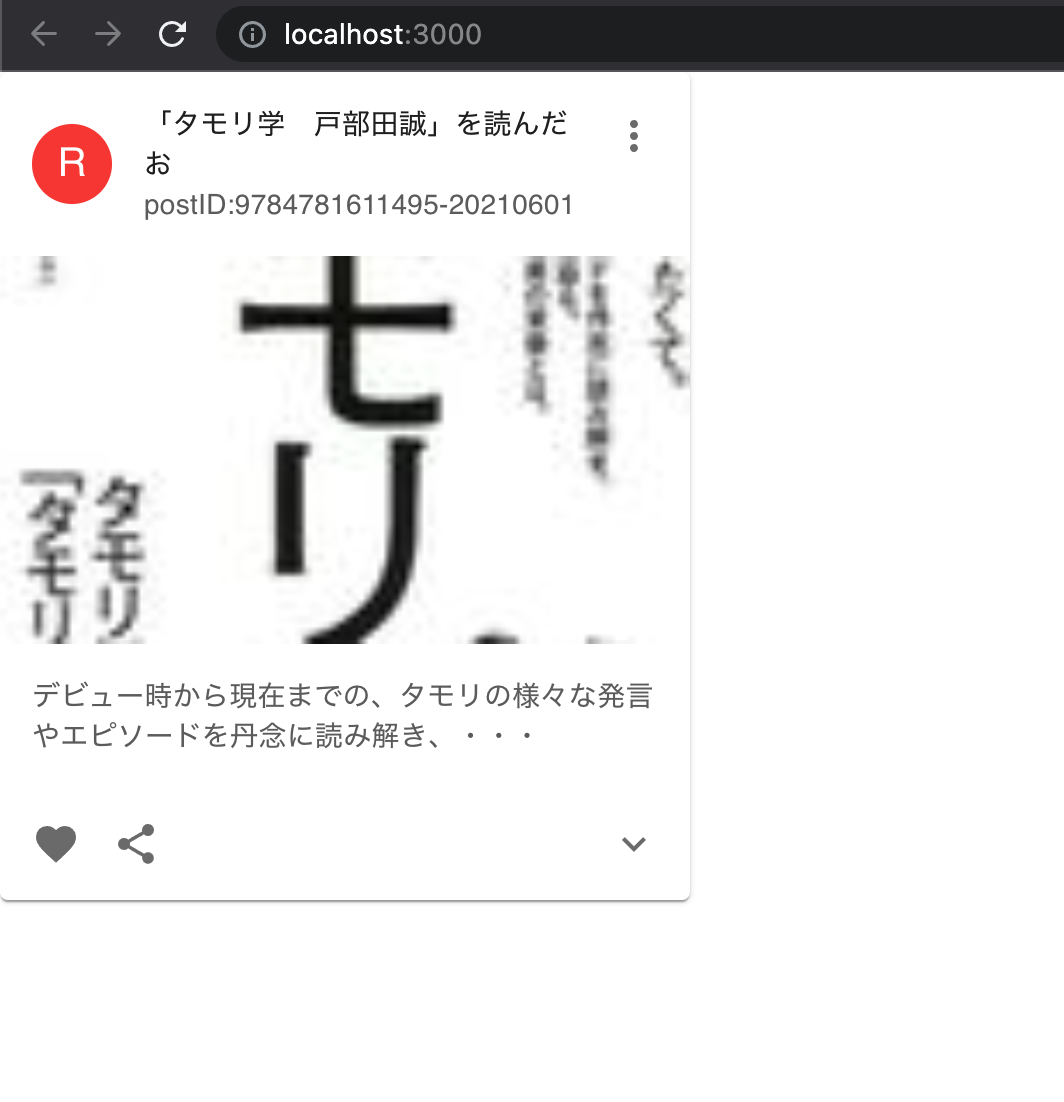
\includegraphics[width=0.6\maxwidth]{./images/03-todo-with-react/sec00332-6.png}%
\reviewimagecaption{カードの単体表示}
\label{image:03-todo-with-react:sec00332-6}
\end{reviewimage}
\begin{starternote}[]{}

ここまでの内容は、GitHub上で、以下のコマンドでクローンできます。

\def\startercodeblockfontsize{}
\begin{starterterminal}[]{GitHub}\seqsplit{\textgreater{} git clone {-}b 02\textunderscore{}Component{-}Cardboard https://github.com/yaruo{-}react{-}redux/yaruo{-}diary.git}\end{starterterminal}
\end{starternote}

\subsection{リファクタリング1(サンプルデータ全表示)}
\keeplastskip{
  \label{sec:3-3-5}
  \label{sec-0333}
  \par\nobreak
}

用意してあるサンプルデータを初期値として使用し、カード一覧へ表示しましょう。

\vspace*{\baselineskip}

先ほどデータ型を記入したデータファイル「src/diaryDate.ts」へサンプル用データをコピペします。
サンプルアプリケーションのGitHubサイトにありますので使ってください。

次に、「App.tsx」を変更します。

\begin{starterenumerate}
\item initialDataは不要になったので削除。
\item 作成したサンプルデータをインポート。
\item DiaryBoardコンポーネントをpropsを受け付けるよう変更
\end{starterenumerate}

変更後の「Appコンポーネント」は、こちらになります。

\def\startercodeblockfontsize{}
\begin{starterprogram}[]{変更後のAppコンポーネント}\seqsplit{  import React from 'react';
  import CssBaseline from '@mui/material/CssBaseline';
  import \{ createTheme, ThemeProvider \} from '@mui/material/styles';

  import diaries from '../diaryData';
  import DiaryBoard from './DiaryBoard';

  const theme = createTheme();

  const App = () =\textgreater{} (
    \textless{}ThemeProvider theme=\{theme\}\textgreater{}
      \textless{}CssBaseline /\textgreater{}
      \textless{}DiaryBoard diaries=\{diaries\} /\textgreater{}
    \textless{}/ThemeProvider\textgreater{}
  );

  export default App;}\end{starterprogram}

「DiaryBoardコンポーネント」を変更します。

\begin{starterenumerate}
\item propsでDiary型の配列を受け付ける
\item DiaryCardコンポーネントを使って各データを表示する
\item Footerのべた書き文字列をアプリケーション用に変更する。
\end{starterenumerate}

変更した「DiaryBoardコンポーネント」が、こちらになります。

\def\startercodeblockfontsize{}
\begin{starterprogram}[]{変更後のDiaryBoardコンポーネント}\seqsplit{  import React from 'react';
  import AppBar from '@mui/material/AppBar';
  import Grid from '@mui/material/Grid';
  import Box from '@mui/material/Box';
  import Toolbar from '@mui/material/Toolbar';
  import Typography from '@mui/material/Typography';
  import Container from '@mui/material/Container';
  import Link from '@mui/material/Link';

  import \{ Diary \} from '../diaryData';
  import DiaryCard from './DiaryCard';

  export type DiaryBoardProps = \{
    diaries: Diary[];
  \};

  const Copyright = () =\textgreater{} (
    \textless{}Typography variant='body2' color='text.secondary' align='center'\textgreater{}
      \{'Copyright © '\}
      \textless{}Link color='inherit' href='https://mui.com/'\textgreater{}
        やる夫が読書します。
      \textless{}/Link\textgreater{}
      \{` \textdollar{}\{new Date().getFullYear()\}.`\}
    \textless{}/Typography\textgreater{}
  );

  const DiaryBoard = (props: DiaryBoardProps) =\textgreater{} \{
    const \{ diaries \} = props;

    return (
      \textless{}\textgreater{}
        \textless{}AppBar position='relative'\textgreater{}
          \textless{}Toolbar\textgreater{}
            \textless{}Typography variant='h6' color='inherit' noWrap\textgreater{}
              やる夫の読書日記
            \textless{}/Typography\textgreater{}
          \textless{}/Toolbar\textgreater{}
        \textless{}/AppBar\textgreater{}
        \textless{}main\textgreater{}
          \textless{}Container sx=\{\{ py: 8 \}\} maxWidth='md'\textgreater{}
            \textless{}Grid container spacing=\{4\}\textgreater{}
              \{diaries.map((diary) =\textgreater{} (
                \textless{}Grid item key=\{diary.diaryId\} xs=\{12\} sm=\{6\} md=\{4\}\textgreater{}
                  \textless{}DiaryCard diary=\{diary\} /\textgreater{}
                \textless{}/Grid\textgreater{}
              ))\}
            \textless{}/Grid\textgreater{}
          \textless{}/Container\textgreater{}
        \textless{}/main\textgreater{}
        \{/* Footer */\}
        \textless{}Box sx=\{\{ bgcolor: 'background.paper', p: 6 \}\} component='footer'\textgreater{}
          \textless{}Typography variant='h6' align='center' gutterBottom\textgreater{}
            やる夫の読書日記
          \textless{}/Typography\textgreater{}
          \textless{}Typography
            variant='subtitle1'
            align='center'
            color='text.secondary'
            component='p'
          \textgreater{}
            お前らも本読んだ良いお〜!
          \textless{}/Typography\textgreater{}
          \textless{}Copyright /\textgreater{}
        \textless{}/Box\textgreater{}
        \{/* End footer */\}
      \textless{}/\textgreater{}
    );
  \};

  export default DiaryBoard;}\end{starterprogram}

変更が完了しましたら、動作確認をします。以下のように表示されると成功です。


\clearpage

\begin{reviewimage}%%diaryBoad_done
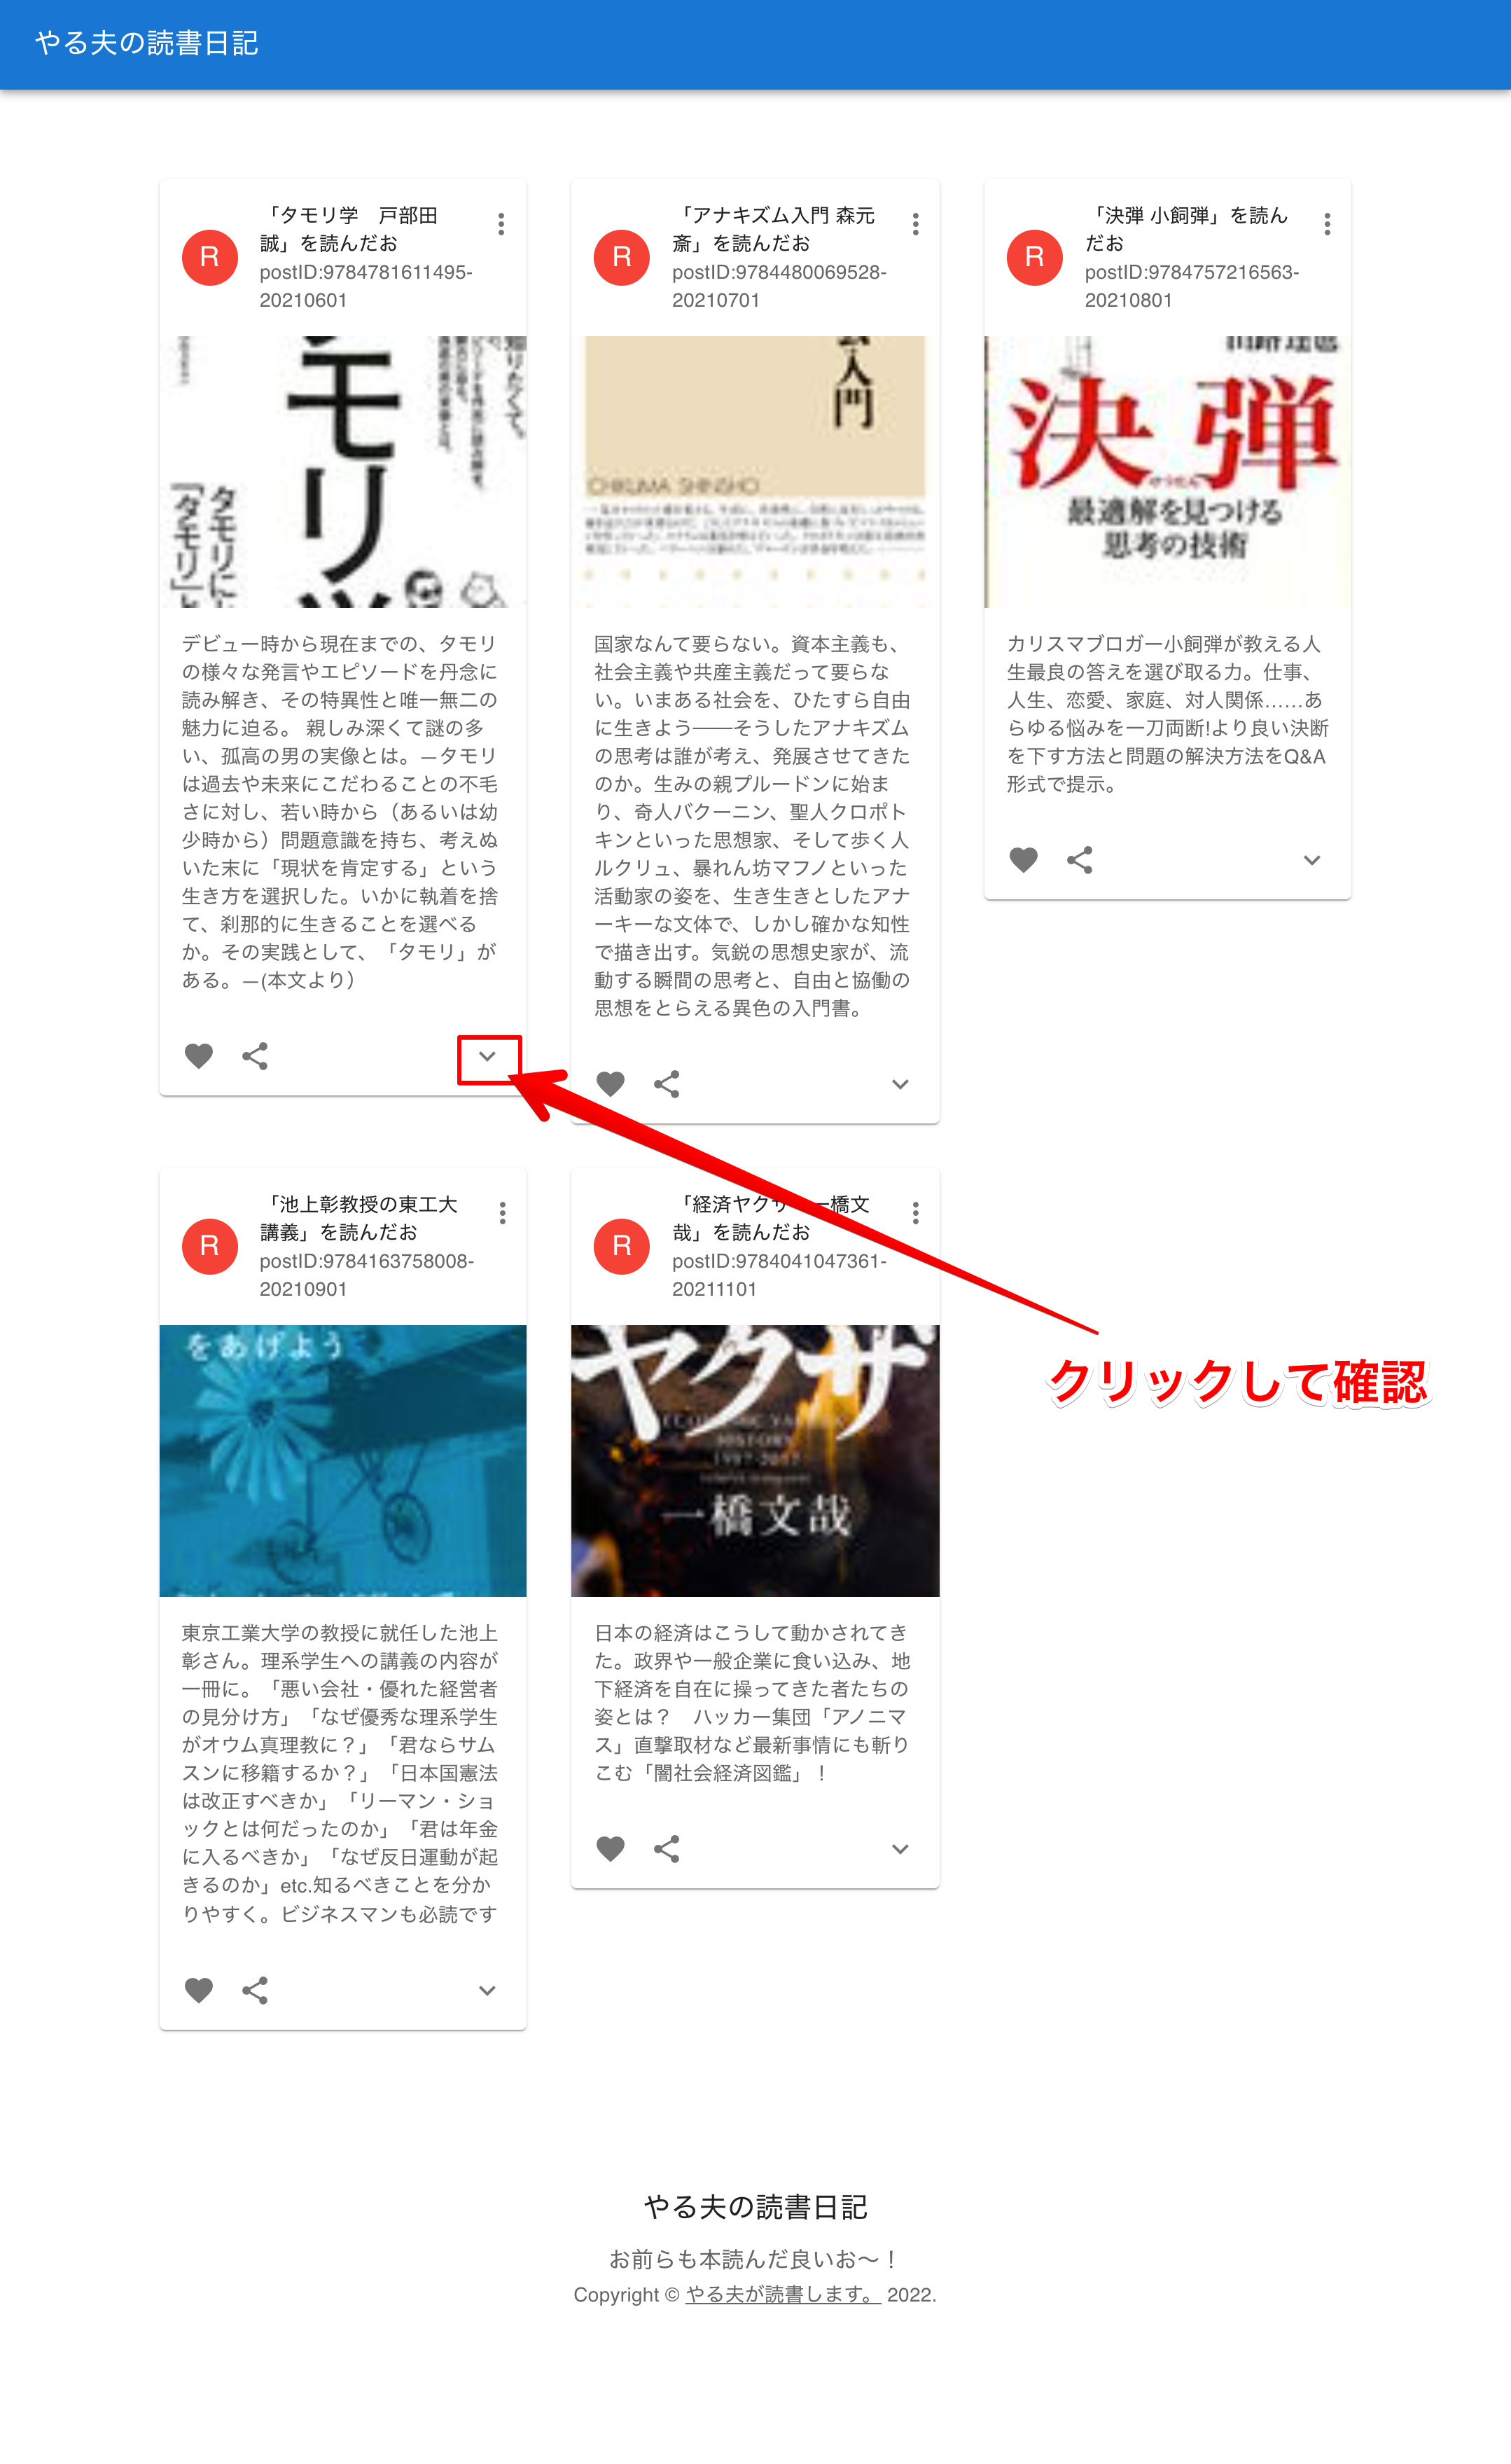
\includegraphics[width=0.7\maxwidth]{./images/03-todo-with-react/diaryBoad_done.png}%
\reviewimagecaption{全データ表示}
\label{image:03-todo-with-react:diaryBoad_done}
\end{reviewimage}

\subsection{リファクタリング2(カードヘッダを別コンポーネントへ)}
\keeplastskip{
  \label{sec:3-3-6}
  \label{sec-0336}
  \par\nobreak
}

「DiaryCardコンポーネント」のタイトルの右側にある「縦の3点」アイコンをクリックしても、今は何も起こりません。
このアイコンボタンを利用して、「編集・削除」の機能を持たせます。

MUIサイトのコンポーネント例の「Menu」にあるものを拝借します。

\begin{reviewimage}%%mui010-card-Menu
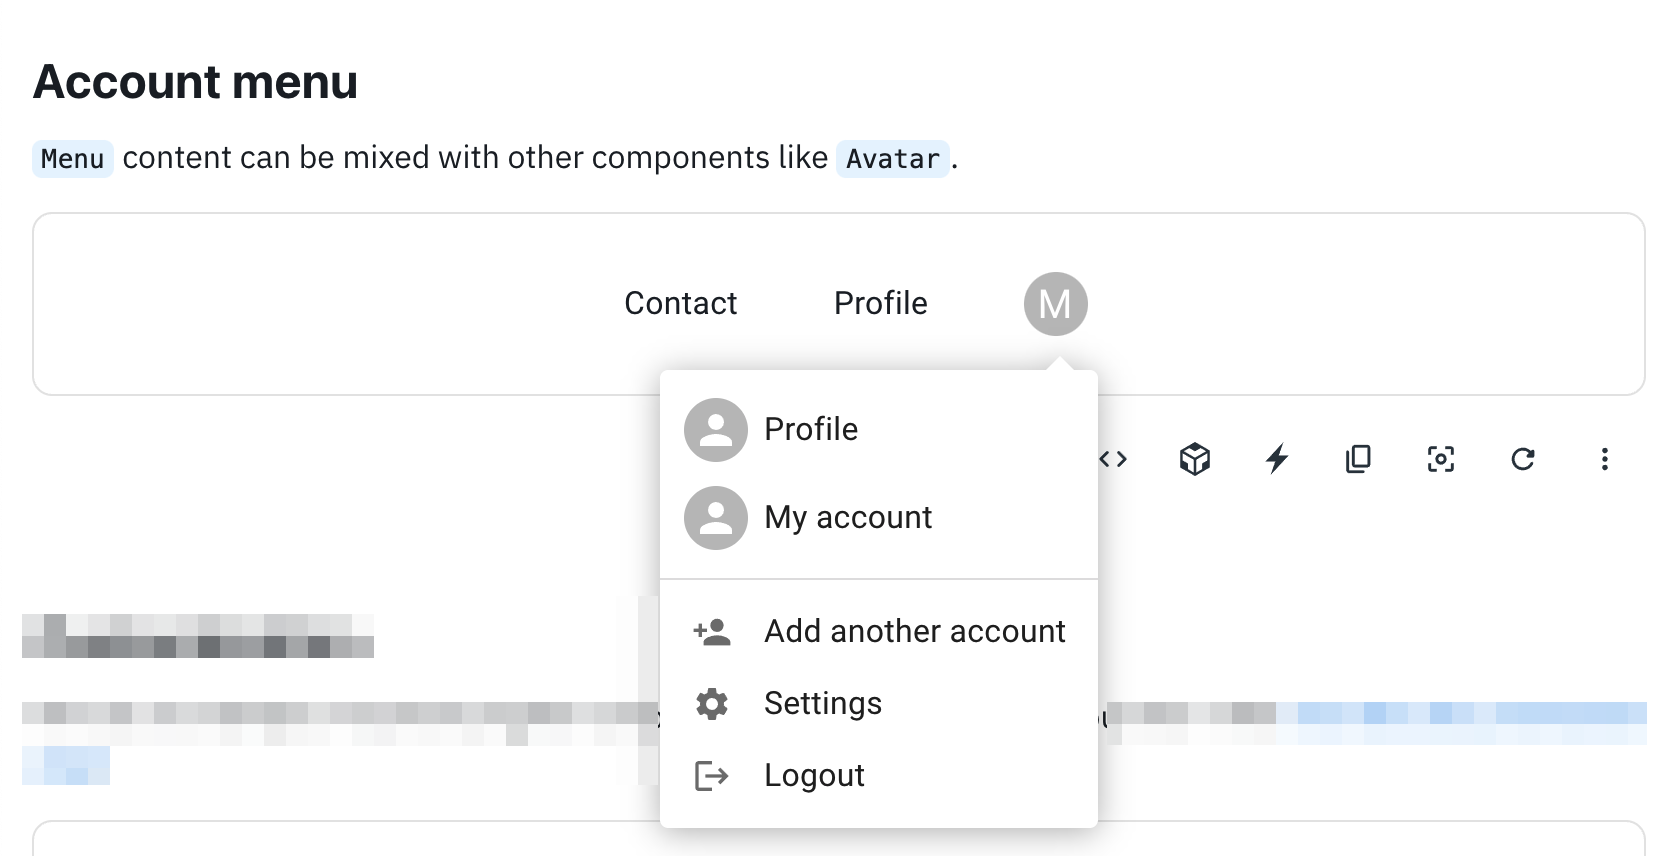
\includegraphics[width=0.6\maxwidth]{./images/03-todo-with-react/mui010-card-Menu.png}%
\reviewimagecaption{アイコンボタンでポップアップメニュー}
\label{image:03-todo-with-react:mui010-card-Menu}
\end{reviewimage}
\vspace*{\baselineskip}

「CardHeader」を再利用することはないでしょうが、管理・メンテナンスを考えて別コンポーネントにします。

\vspace*{\baselineskip}

\begin{starterenumerate}
\item 「DiaryCardHeader.tsx」ファイルを作成しコンポーネントのテンプレを書く
\item 「DiaryCard.tsx」から、CardHeader部分を「DiaryCardHeader.tsx」切り出し
\item 「DiaryCardコンポーネント」に「DiaryCardHeaderコンポーネント」をインポートして使用
\end{starterenumerate}

変更が完了したファイルは、このようになります。

\def\startercodeblockfontsize{}
\begin{starterprogram}[]{DiaryCardHeaderコンポーネント}\seqsplit{   import React from 'react';
  import CardHeader from '@mui/material/CardHeader';
  import Avatar from '@mui/material/Avatar';
  import \{ red \} from '@mui/material/colors';
  import MoreVertIcon from '@mui/icons{-}material/MoreVert';
  import IconButton from '@mui/material/IconButton';

  export type DiaryCardHeaderProps = \{
    diaryId: string;
    title: string;
    postDate: string;
  \};

  const DiaryCardHeader = (props: DiaryCardHeaderProps) =\textgreater{} \{
    const \{ diaryId, title, postDate \} = props;
    return (
      \textless{}CardHeader
        avatar=\{
          \textless{}Avatar sx=\{\{ bgcolor: red[500] \}\} aria{-}label='recipe'\textgreater{}
            R
          \textless{}/Avatar\textgreater{}
        \}
        action=\{
          \textless{}IconButton aria{-}label='settings'\textgreater{}
            \textless{}MoreVertIcon /\textgreater{}
          \textless{}/IconButton\textgreater{}
        \}
        title=\{title\}
        subheader=\{`postID:\textdollar{}\{diaryId\}{-}\textdollar{}\{postDate\}`\}
      /\textgreater{}
    );
  \};

  export default DiaryCardHeader;
 //\}

 「DiaryCardコンポーネント」は、このようになります。

 //list[][DiaryCardコンポーネントのCardHeaderがあった部分]\{
   return (
    \textless{}Card sx=\{\{ maxWidth: 345 \}\}\textgreater{}
      \textless{}DiaryCardHeader diaryId=\{diaryId\} title=\{title\} postDate=\{postDate\} /\textgreater{}
      \textless{}CardMedia
        component='img'
        height='194'
        image=\{imageUrl\}
        alt=\{imageLabel\}
      /\textgreater{}
      \textless{}CardContent\textgreater{}
        \textless{}Typography variant='body2' color='text.secondary'\textgreater{}
          \{mainContent\}
        \textless{}/Typography\textgreater{}
      \textless{}/CardContent\textgreater{}}\end{starterprogram}

この時点で動作確認を行います。無事に表示されていれば良いです。

\subsubsection*{DiaryBoardコンポーネントにメニューを組み込む}
\keeplastskip{
  \label{sec:3-3-6-1}
  \label{sec-0336-1}
  \par\nobreak
}

MUIのサイトからメニュー部分のコードを拝借して「DiaryCardHeaderコンポーネント」に追加しましょう。
やりたいことは「編集、削除」ですので、メニュー項目(MenuItem)は2つで良いです。


\clearpage

\begin{reviewimage}%%mui011-card-MenuCode
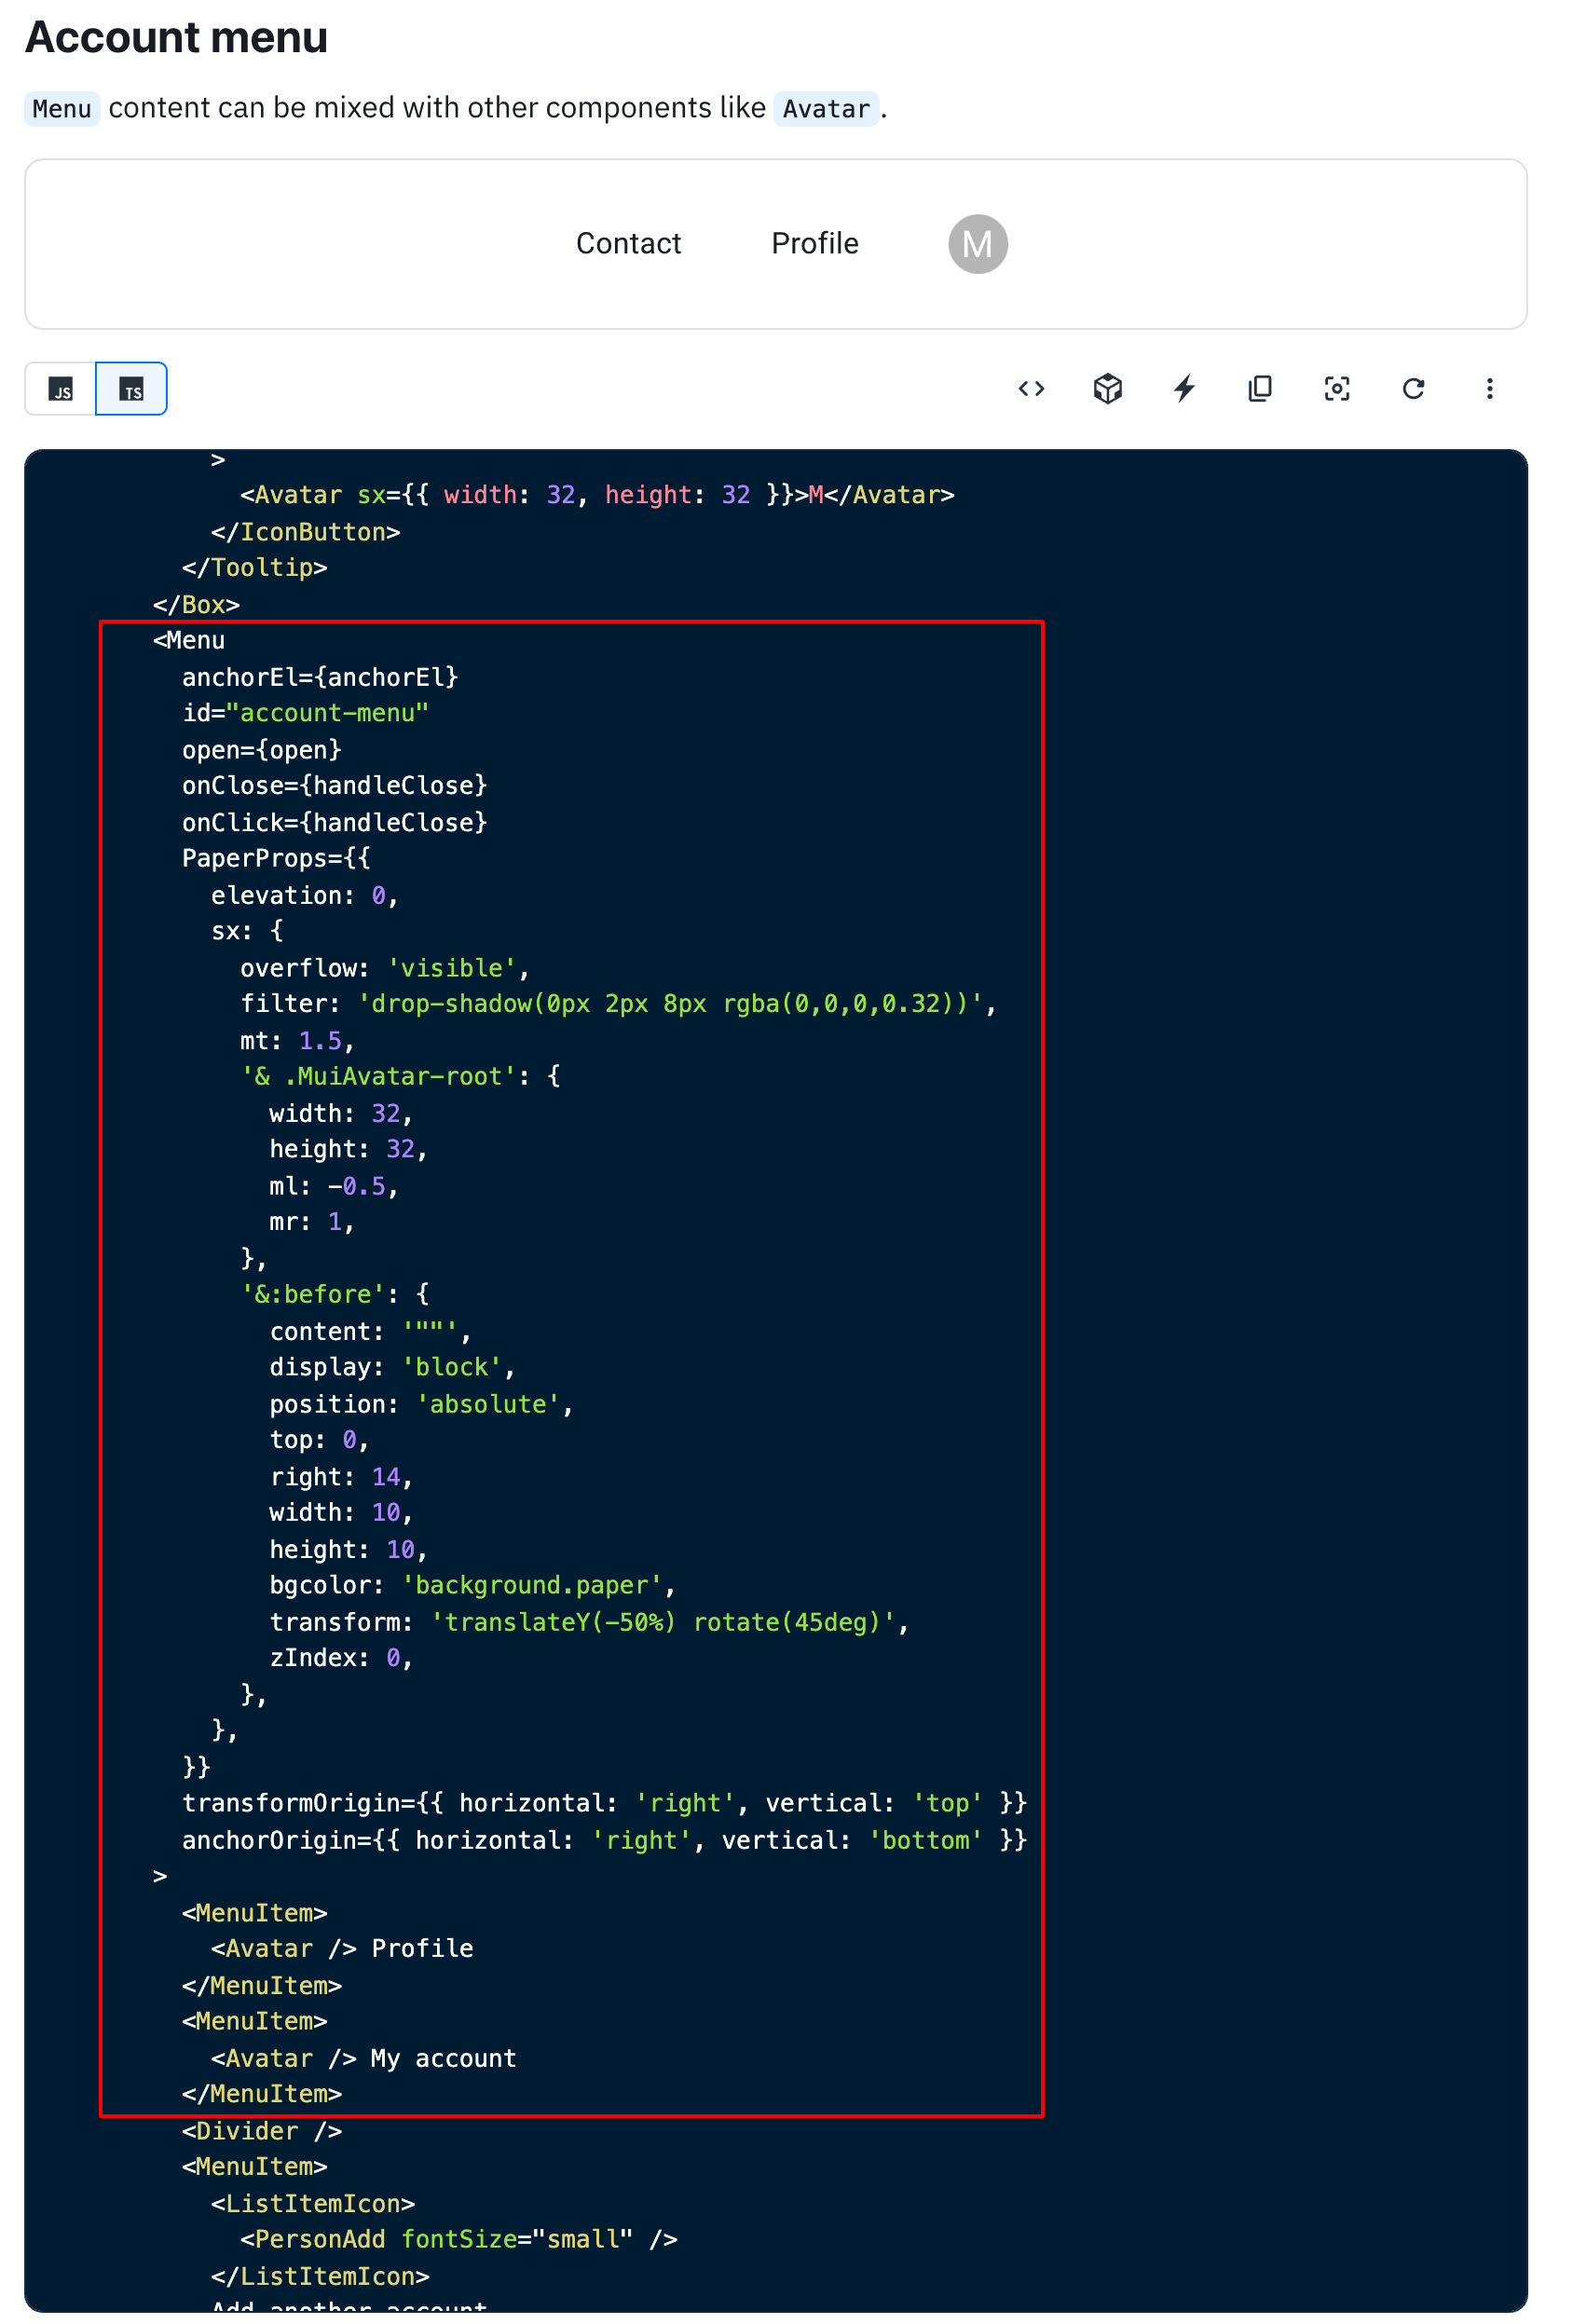
\includegraphics[width=0.7\maxwidth]{./images/03-todo-with-react/mui011-card-MenuCode.png}%
\reviewimagecaption{MUIのMenuサンプル}
\label{image:03-todo-with-react:mui011-card-MenuCode}
\end{reviewimage}

拝借するコードは、「CardHeader」と同じ階層に貼り付けますが、その場合「Jsxはひとつの要素」と怒られますので、
トップ階層に「\textless{}\textgreater{}\textless{}/\textgreater{}」を追加します。

\vspace*{\baselineskip}

必要なMUIのコンポーネント、アイコンもインポートするのですが、アイコンは、

\begin{description}
\item[編集アイコン] \mbox{} \\
import EditIcon from '@mui/icons{-}material/Edit';
\item[削除アイコン] \mbox{} \\
import DeleteForeverIcon from '@mui/icons{-}material/DeleteForever';
\end{description}

を使い、Avatarコンポーネントではなく「ListItemIconコンポーネント」を使います。サンプルメニューの
区切り線の下の部分で使われています。

\vspace*{\baselineskip}

最後は、「AccountMenuコンポーネント」の関数(HTML内に埋め込まれています)も忘れずにコピペしてください。

\vspace*{\baselineskip}

handleClick関数は、MoreVertIconの親要素のIconButtonの「onClick」に追加します。

ここまでの変更が完了すると「DiaryCardHeaderコンポーネント」は、このようになります。

\def\startercodeblockfontsize{}
\begin{starterprogram}[]{変更完了のDiaryCardHeaderコンポーネント}\seqsplit{  import React from 'react';
  import CardHeader from '@mui/material/CardHeader';
  import Avatar from '@mui/material/Avatar';
  import \{ red \} from '@mui/material/colors';
  import Menu from '@mui/material/Menu';
  import MenuItem from '@mui/material/MenuItem';
  import ListItemIcon from '@mui/material/ListItemIcon';
  import MoreVertIcon from '@mui/icons{-}material/MoreVert';
  import EditIcon from '@mui/icons{-}material/Edit';
  import DeleteForeverIcon from '@mui/icons{-}material/DeleteForever';
  import IconButton from '@mui/material/IconButton';

  export type DiaryCardHeaderProps = \{
    diaryId: string;
    title: string;
    postDate: string;
  \};

  const DiaryCardHeader = (props: DiaryCardHeaderProps) =\textgreater{} \{
    const \{ diaryId, title, postDate \} = props;
    const [anchorEl, setAnchorEl] = React.useState\textless{}null \textbar{} HTMLElement\textgreater{}(null);
    const open = Boolean(anchorEl);
    const handleClick = (event: React.MouseEvent\textless{}HTMLElement\textgreater{}) =\textgreater{} \{
      setAnchorEl(event.currentTarget);
    \};
    const handleClose = () =\textgreater{} \{
      setAnchorEl(null);
    \};

    return (
      \textless{}\textgreater{}
        \textless{}CardHeader
          avatar=\{
            \textless{}Avatar sx=\{\{ bgcolor: red[500] \}\} aria{-}label='recipe'\textgreater{}
              R
            \textless{}/Avatar\textgreater{}
          \}
          action=\{
            \textless{}IconButton aria{-}label='settings' onClick=\{handleClick\}\textgreater{}
              \textless{}MoreVertIcon /\textgreater{}
            \textless{}/IconButton\textgreater{}
          \}
          title=\{title\}
          subheader=\{`postID:\textdollar{}\{diaryId\}{-}\textdollar{}\{postDate\}`\}
        /\textgreater{}
        \textless{}Menu
          anchorEl=\{anchorEl\}
          id='account{-}menu'
          open=\{open\}
          onClose=\{handleClose\}
          onClick=\{handleClose\}
          PaperProps=\{\{
            elevation: 0,
            sx: \{
              overflow: 'visible',
              filter: 'drop{-}shadow(0px 2px 8px rgba(0,0,0,0.32))',
              mt: 1.5,
              '\& .MuiAvatar{-}root': \{
                width: 32,
                height: 32,
                ml: {-}0.5,
                mr: 1,
              \},
              '\&:before': \{
                content: '""',
                display: 'block',
                position: 'absolute',
                top: 0,
                right: 14,
                width: 10,
                height: 10,
                bgcolor: 'background.paper',
                transform: 'translateY({-}50\%) rotate(45deg)',
                zIndex: 0,
              \},
            \},
          \}\}
          transformOrigin=\{\{ horizontal: 'right', vertical: 'top' \}\}
          anchorOrigin=\{\{ horizontal: 'right', vertical: 'bottom' \}\}
        \textgreater{}
          \textless{}MenuItem\textgreater{}
            \textless{}ListItemIcon\textgreater{}
              \textless{}EditIcon fontSize='small' /\textgreater{}
            \textless{}/ListItemIcon\textgreater{}
            編集
          \textless{}/MenuItem\textgreater{}
          \textless{}MenuItem\textgreater{}
            \textless{}ListItemIcon\textgreater{}
              \textless{}DeleteForeverIcon fontSize='small' /\textgreater{}
            \textless{}/ListItemIcon\textgreater{}
            削除
          \textless{}/MenuItem\textgreater{}
        \textless{}/Menu\textgreater{}
      \textless{}/\textgreater{}
    );
  \};

  export default DiaryCardHeader;}\end{starterprogram}

ここまでの変更を動作確認します。「縦の3点アイコン」をクリックするとメニューが表示されますか?


\clearpage

\begin{reviewimage}%%mui012-card-MenuStep1
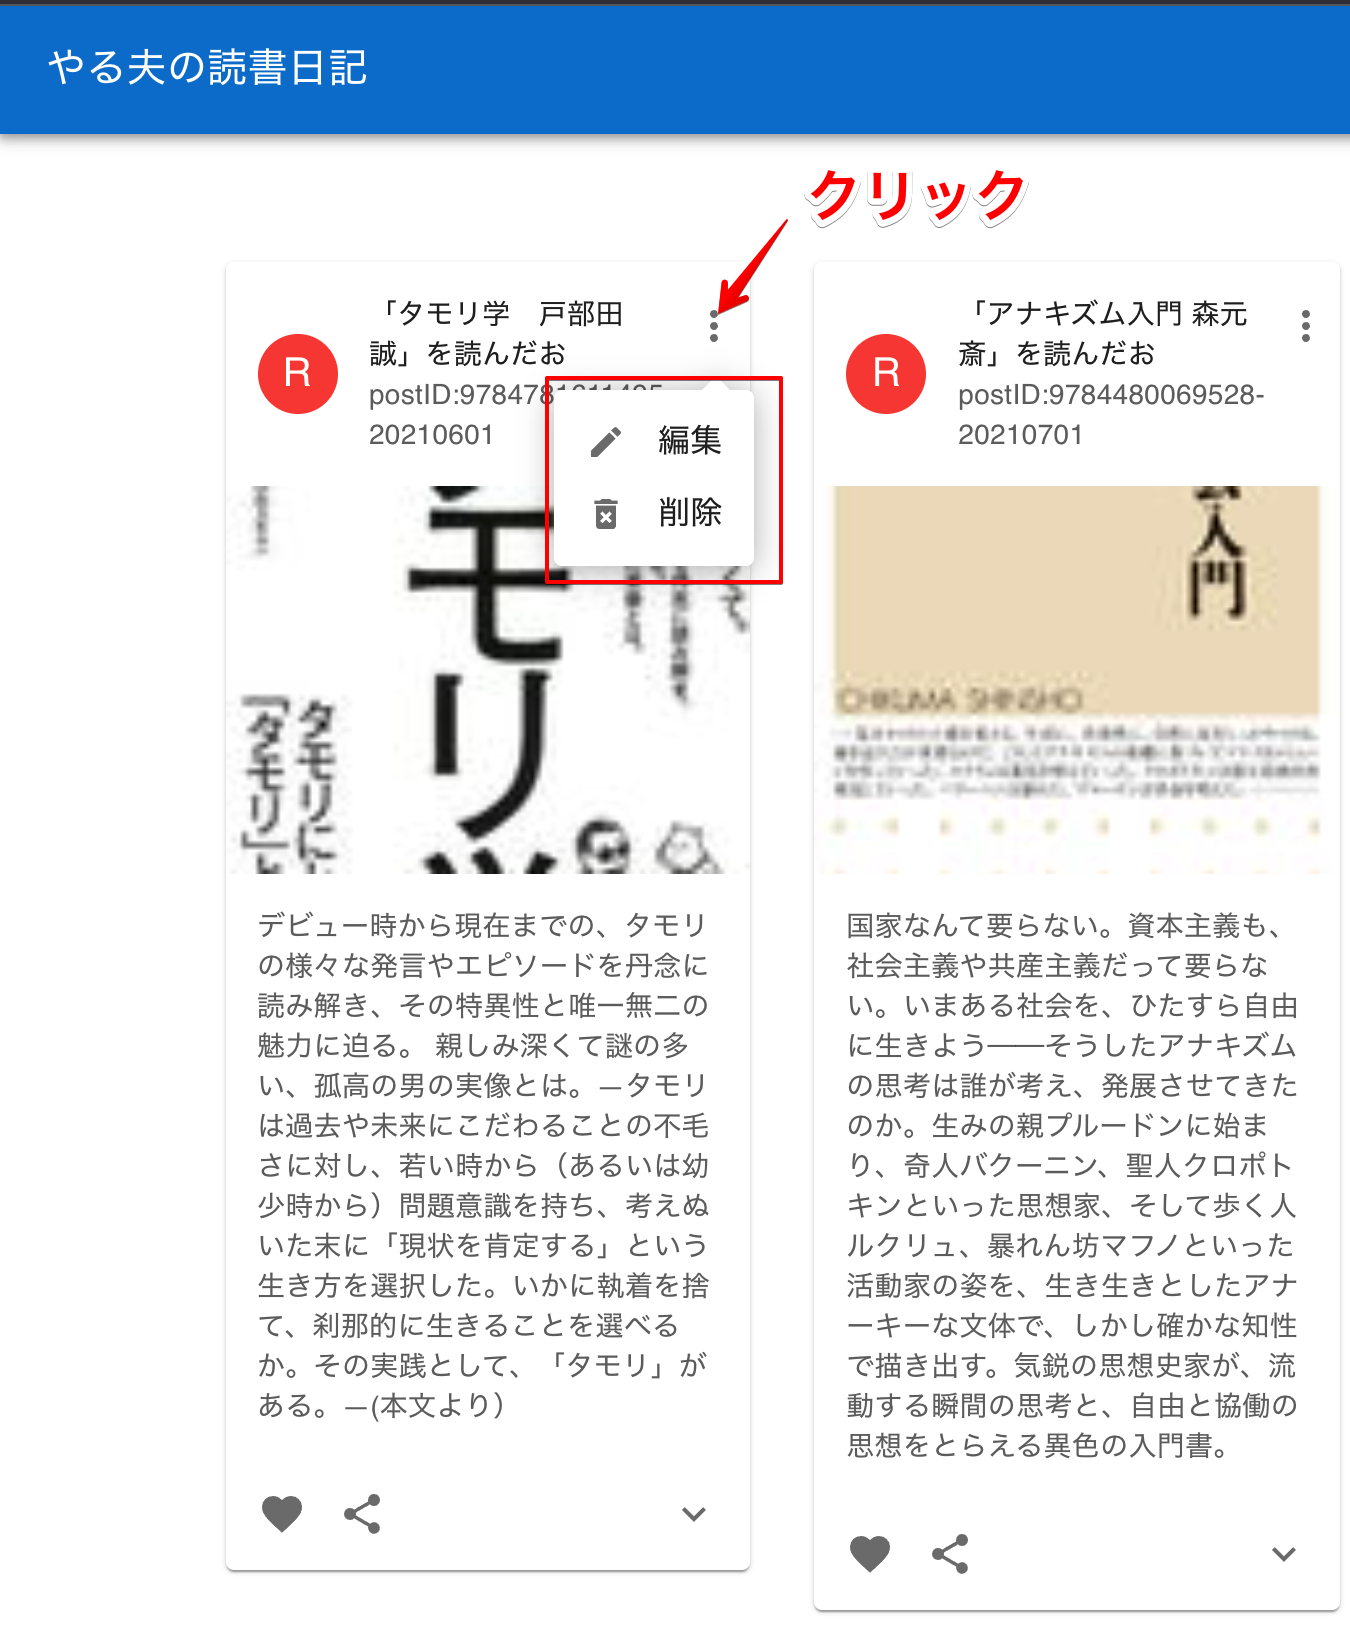
\includegraphics[width=0.7\maxwidth]{./images/03-todo-with-react/mui012-card-MenuStep1.png}%
\reviewimagecaption{クリックするとメニューが表示される}
\label{image:03-todo-with-react:mui012-card-MenuStep1}
\end{reviewimage}

メニューが無事表示されたので、のちほど実際の関数に置き換えるとして、テストとしてアラートを出してみます。
「編集・削除」のMenuItemコンポーネントに「onClick」を追加し対応する関数を書きます。

\vspace*{\baselineskip}

ただし、削除がクリックされたときには「本当に削除しますか?」と確認のダイアログを出すようにします。
ダイアログは、MUIサイトの「Dialog」から「Transitions」を拝借します。

\begin{reviewimage}%%mui013-card-deleteDialog
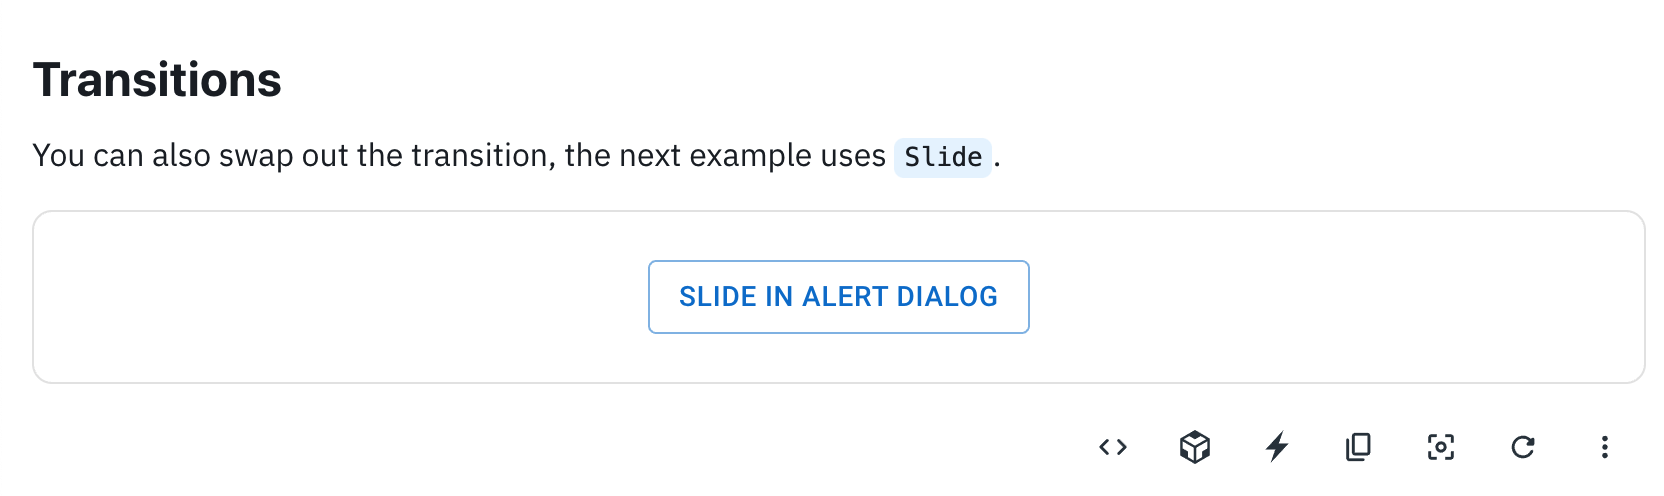
\includegraphics[width=0.6\maxwidth]{./images/03-todo-with-react/mui013-card-deleteDialog.png}%
\reviewimagecaption{MUIサイトのTransitionsダイアログ}
\label{image:03-todo-with-react:mui013-card-deleteDialog}
\end{reviewimage}
\vspace*{\baselineskip}

「Dialogコンポーネント」のソースコードを表示し、\textless{}Dialog\textgreater{} \textasciitilde{} \textless{}/Dialog\textgreater{}を\textless{}/Menu\textgreater{}の下へコピペします。
不要なものは削除し、「キャンセル」、「削除」のボタンを作成します。もちろん、必要な関数もコピペします。

\vspace*{\baselineskip}

コピペすると、メニューの開閉状態の「open」とダイアログ表示状態の「open」が重複しますので、それぞれ
「openMenu」、「openDialog」に名前を変えます。また閉じる関数「handleClose」も重複しますので名前を変えます。

\vspace*{\baselineskip}

Menuの「削除」をクリック {-}\textgreater{} 確認ダイアログ表示 {-}\textgreater{} 削除 {-}\textgreater{} アラート表示になるように関数呼び出します。

\vspace*{\baselineskip}

ここまでの変更が完了しましたら動作確認します。

編集メニューをクリックしたときにアラートはでましたか?\\[0pt]
削除メニューをクリックしたときに確認ダイアログが表示しましたか?\\[0pt]
確認ダイアログの削除をクリックしたときにアラートはでましたか?


\clearpage

\begin{reviewimage}%%mui014-card-deleteDialog-done
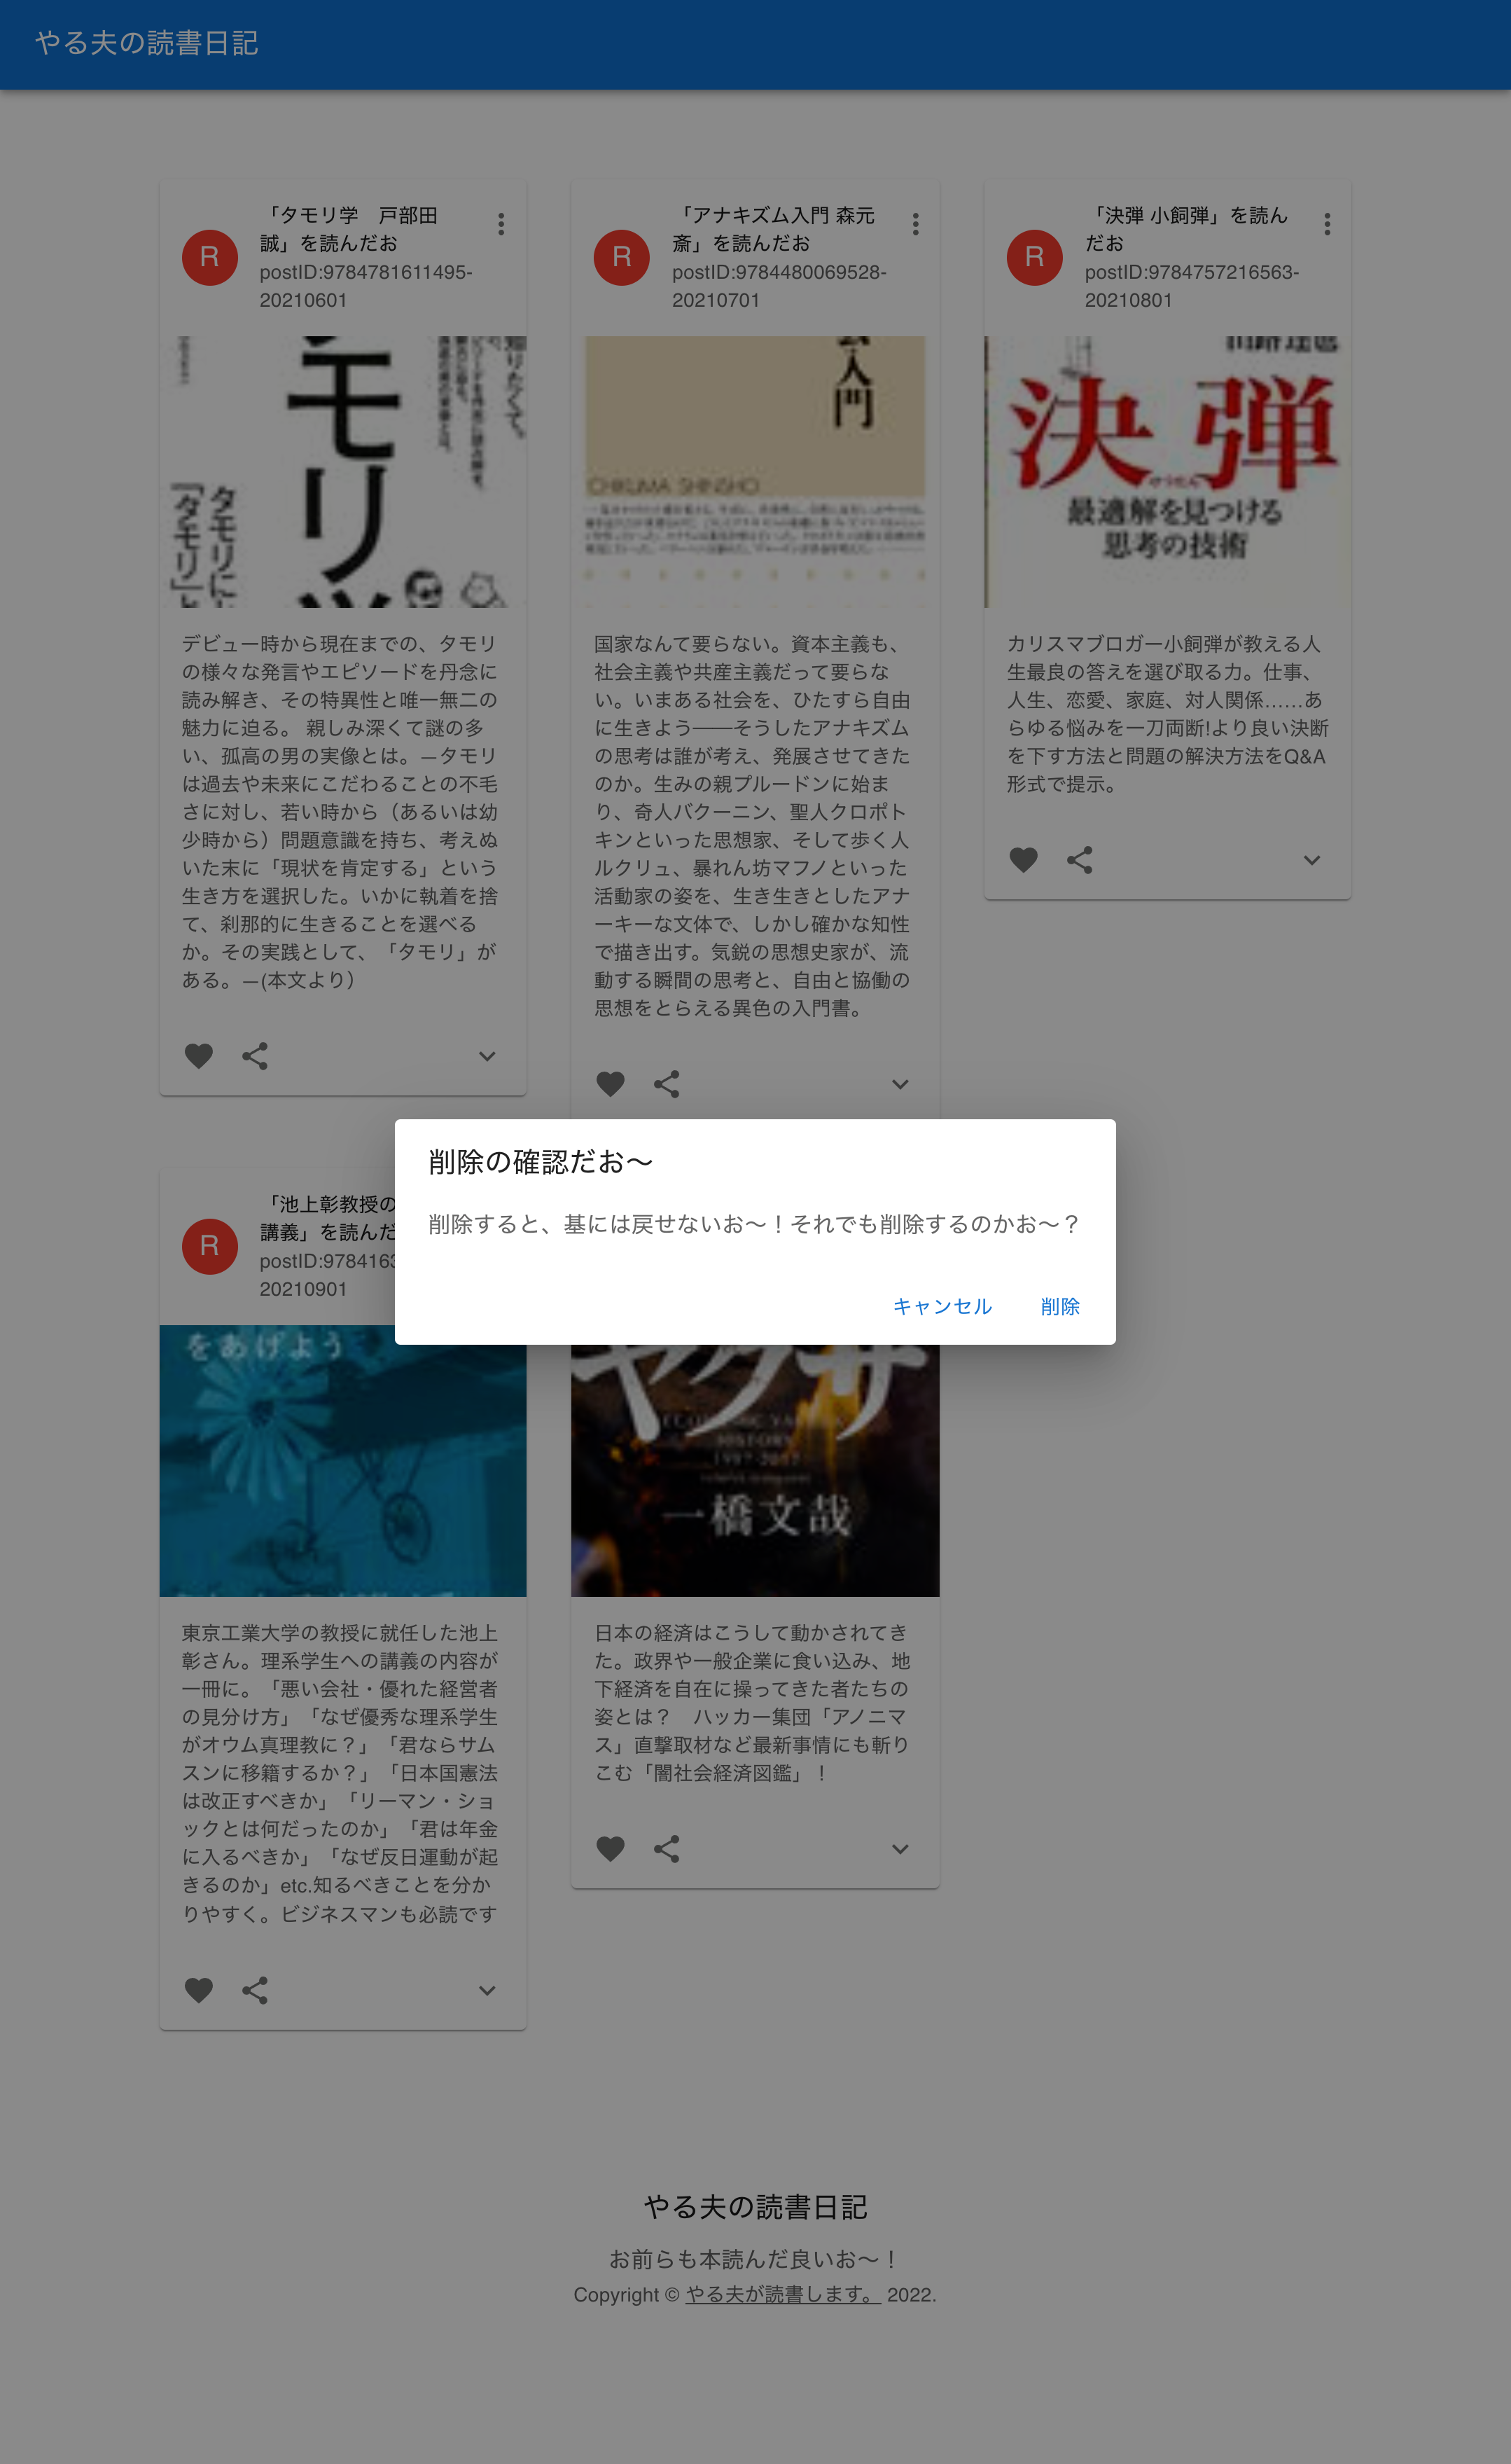
\includegraphics[width=0.7\maxwidth]{./images/03-todo-with-react/mui014-card-deleteDialog-done.png}%
\reviewimagecaption{削除確認ダイアログの表示}
\label{image:03-todo-with-react:mui014-card-deleteDialog-done}
\end{reviewimage}

\subsubsection*{DiaryBoardHeaderの見栄え}
\keeplastskip{
  \label{sec:3-3-6-2}
  \label{sec-0336-2}
  \par\nobreak
}

もう少し見栄え良くしたいので、DiaryCardHeaderコンポーネントの、

\begin{starterenumerate}
\item アバターの代わりに投稿月の画像を表示
\item サブタイトルに投稿日を「YYYY年M月D日」で表示
\end{starterenumerate}

を実装します。

\paragraph*{アバターの代わりに投稿付きの表示}\vspace*{\baselineskip}

1月〜12月までのSVG画像は、GitHubサイトにあります。「src/assets/images/month{-}icons」フォルダを作成してコピペしてください。

\vspace*{\baselineskip}

読書日記データの投稿日は「YYYYMMDD」形式の文字列ですので、この文字列からJavaScriptのDateオブジェクトを返す関数を作成します。
また、のちほど作成する読書日記の新規追加・編集時のため日付から「YYYYMMDD」の文字列を作成する関数も合わせて作成します。

どの場所からも使えるように「src/utilities/helper.ts」ファイルを作成し、ここに関数を作成します。

\def\startercodeblockfontsize{}
\begin{starterprogram}[]{src/utilities/helper.ts}\seqsplit{  // DateオブジェクトからYYYYMMDDの文字列へ変換
  export const convertDateToString = (date: Date): string =\textgreater{} \{
    const monthString = `0\textdollar{}\{date.getMonth() + 1\}`.slice({-}2);
    const dayString = `0\textdollar{}\{date.getDate()\}`.slice({-}2);

    return `\textdollar{}\{date.getFullYear()\}\textdollar{}\{monthString\}\textdollar{}\{dayString\}`;
  \};

  // YYYYMMDD文字列からDateオブジェクトへ変換
  export const convertStringToDate = (dateString: string): Date =\textgreater{} \{
    let date;
    if (dateString.length !== 8) \{
      date = new Date();
    \} else \{
      date = new Date(
        +dateString.slice(0, 4),
        +dateString.slice(4, 6) {-} 1,
        +dateString.slice(6)
      );
    \}
    return date;
  \};}\end{starterprogram}

convertStringToDate関数をインポートし、読書日記の「YYYYMMDD」から月を取得し、画像のソースを指定します。
DiaryCardHeaderコンポーネントに追加する関数は、こちらとなります。

\def\startercodeblockfontsize{}
\begin{starterprogram}[]{Dateと文字列の変換関数}\seqsplit{  // DateオブジェクトからYYYYMMDDの文字列へ変換
  export const convertDateToString = (date: Date): string =\textgreater{} \{
    const monthString = `0\textdollar{}\{date.getMonth() + 1\}`.slice({-}2);
    const dayString = `0\textdollar{}\{date.getDate()\}`.slice({-}2);

    return `\textdollar{}\{date.getFullYear()\}\textdollar{}\{monthString\}\textdollar{}\{dayString\}`;
  \};

  // YYYYMMDD文字列からDateオブジェクトへ変換
  export const convertStringToDate = (dateString: string): Date =\textgreater{} \{
    let date;
    if (dateString.length !== 8) \{
      date = new Date();
    \} else \{
      date = new Date(
        +dateString.slice(0, 4),
        +dateString.slice(4, 6) {-} 1,
        +dateString.slice(6)
      );
    \}
    return date;
  \};}\end{starterprogram}

DiaryCardHeaderコンポーネントにアバターのソースを切り替える関数を作成し、
「CardHeaderコンポーネント内Avatarコンポーネント」のsrc要素にします。
ついでに、四角形に変えサイズも大きめにします。

\vspace*{\baselineskip}

追加したコードです。

\def\startercodeblockfontsize{}
\begin{starterprogram}[]{画像の切替とAvatarへの指定}\seqsplit{  // postDate:YYYYMMDDから月を取得し
  const datePosted: Date = convertStringToDate(postDate);
  let avatarSrc;
  // useEffect(() =\textgreater{} \{
  switch (datePosted.getMonth()) \{
    case 0:
      avatarSrc = January;
      break;
    case 1:
      avatarSrc = February;
      break;
    case 2:
      avatarSrc = March;
      break;
    case 3:
      avatarSrc = April;
      break;
    case 4:
      avatarSrc = May;
      break;
    case 5:
      avatarSrc = Jun;
      break;
    case 6:
      avatarSrc = July;
      break;
    case 7:
      avatarSrc = August;
      break;
    case 8:
      avatarSrc = September;
      break;
    case 9:
      avatarSrc = October;
      break;
    case 10:
      avatarSrc = November;
      break;
    case 11:
      avatarSrc = December;
      break;
    default:
      break;
  \}

  return (
    \textless{}\textgreater{}
      \textless{}CardHeader
        avatar=\{
          \textless{}Avatar
            sx=\{\{ width: 58, height: 58 \}\}
            variant='square'
            aria{-}label='recipe'
            src=\{avatarSrc\}
          /\textgreater{}
        \}}\end{starterprogram}

\paragraph*{サブタイトルに投稿日を「YYYY年M月D日」で表示}
「src/utilities/helper.ts」に、「YYYYMMDD」文字列から「YYYY年M月D日」に変換する関数を作成します。

\def\startercodeblockfontsize{}
\begin{starterprogram}[]{YYYY年M月D日文字列の作成関数}\seqsplit{  // YYYYMMDDからYYYY年M月Dに変換
  export const convertToLongDateString = (dateString: string) =\textgreater{} \{
    const date = convertStringToDate(dateString);
    return `\textdollar{}\{date.getFullYear()\}年\textdollar{}\{date.getMonth() + 1\}月\textdollar{}\{date.getDate()\}日`;
  \};}\end{starterprogram}

DiaryCardHeaderコンポーネントへ「convertToLongDateString」をインポートし、投稿日データを表示します。

\def\startercodeblockfontsize{}
\begin{starterprogram}[]{投稿日を表示}\seqsplit{  const posted = convertToLongDateString(postDate);

  \textless{}CardHeader
    avatar=\{
      \textless{}Avatar
        sx=\{\{ width: 58, height: 58 \}\}
        variant='square'
        aria{-}label=\{`投稿日:\textdollar{}\{posted\}`\}  {\reviewballoon{ラベルにも表示}}
        src=\{avatarSrc\}
      /\textgreater{}
    \}
    action=\{
      \textless{}IconButton aria{-}label='settings' onClick=\{handleClick\}\textgreater{}
        \textless{}MoreVertIcon /\textgreater{}
      \textless{}/IconButton\textgreater{}
    \}
    title=\{title\}
    subheader=\{posted\} {\reviewballoon{サブタイトルに投稿日}}
  /\textgreater{}}\end{starterprogram}

さて、ここまでの変更が完了しましたら、動作確認を行います。


\clearpage

\begin{reviewimage}%%mui015-card-Header-done
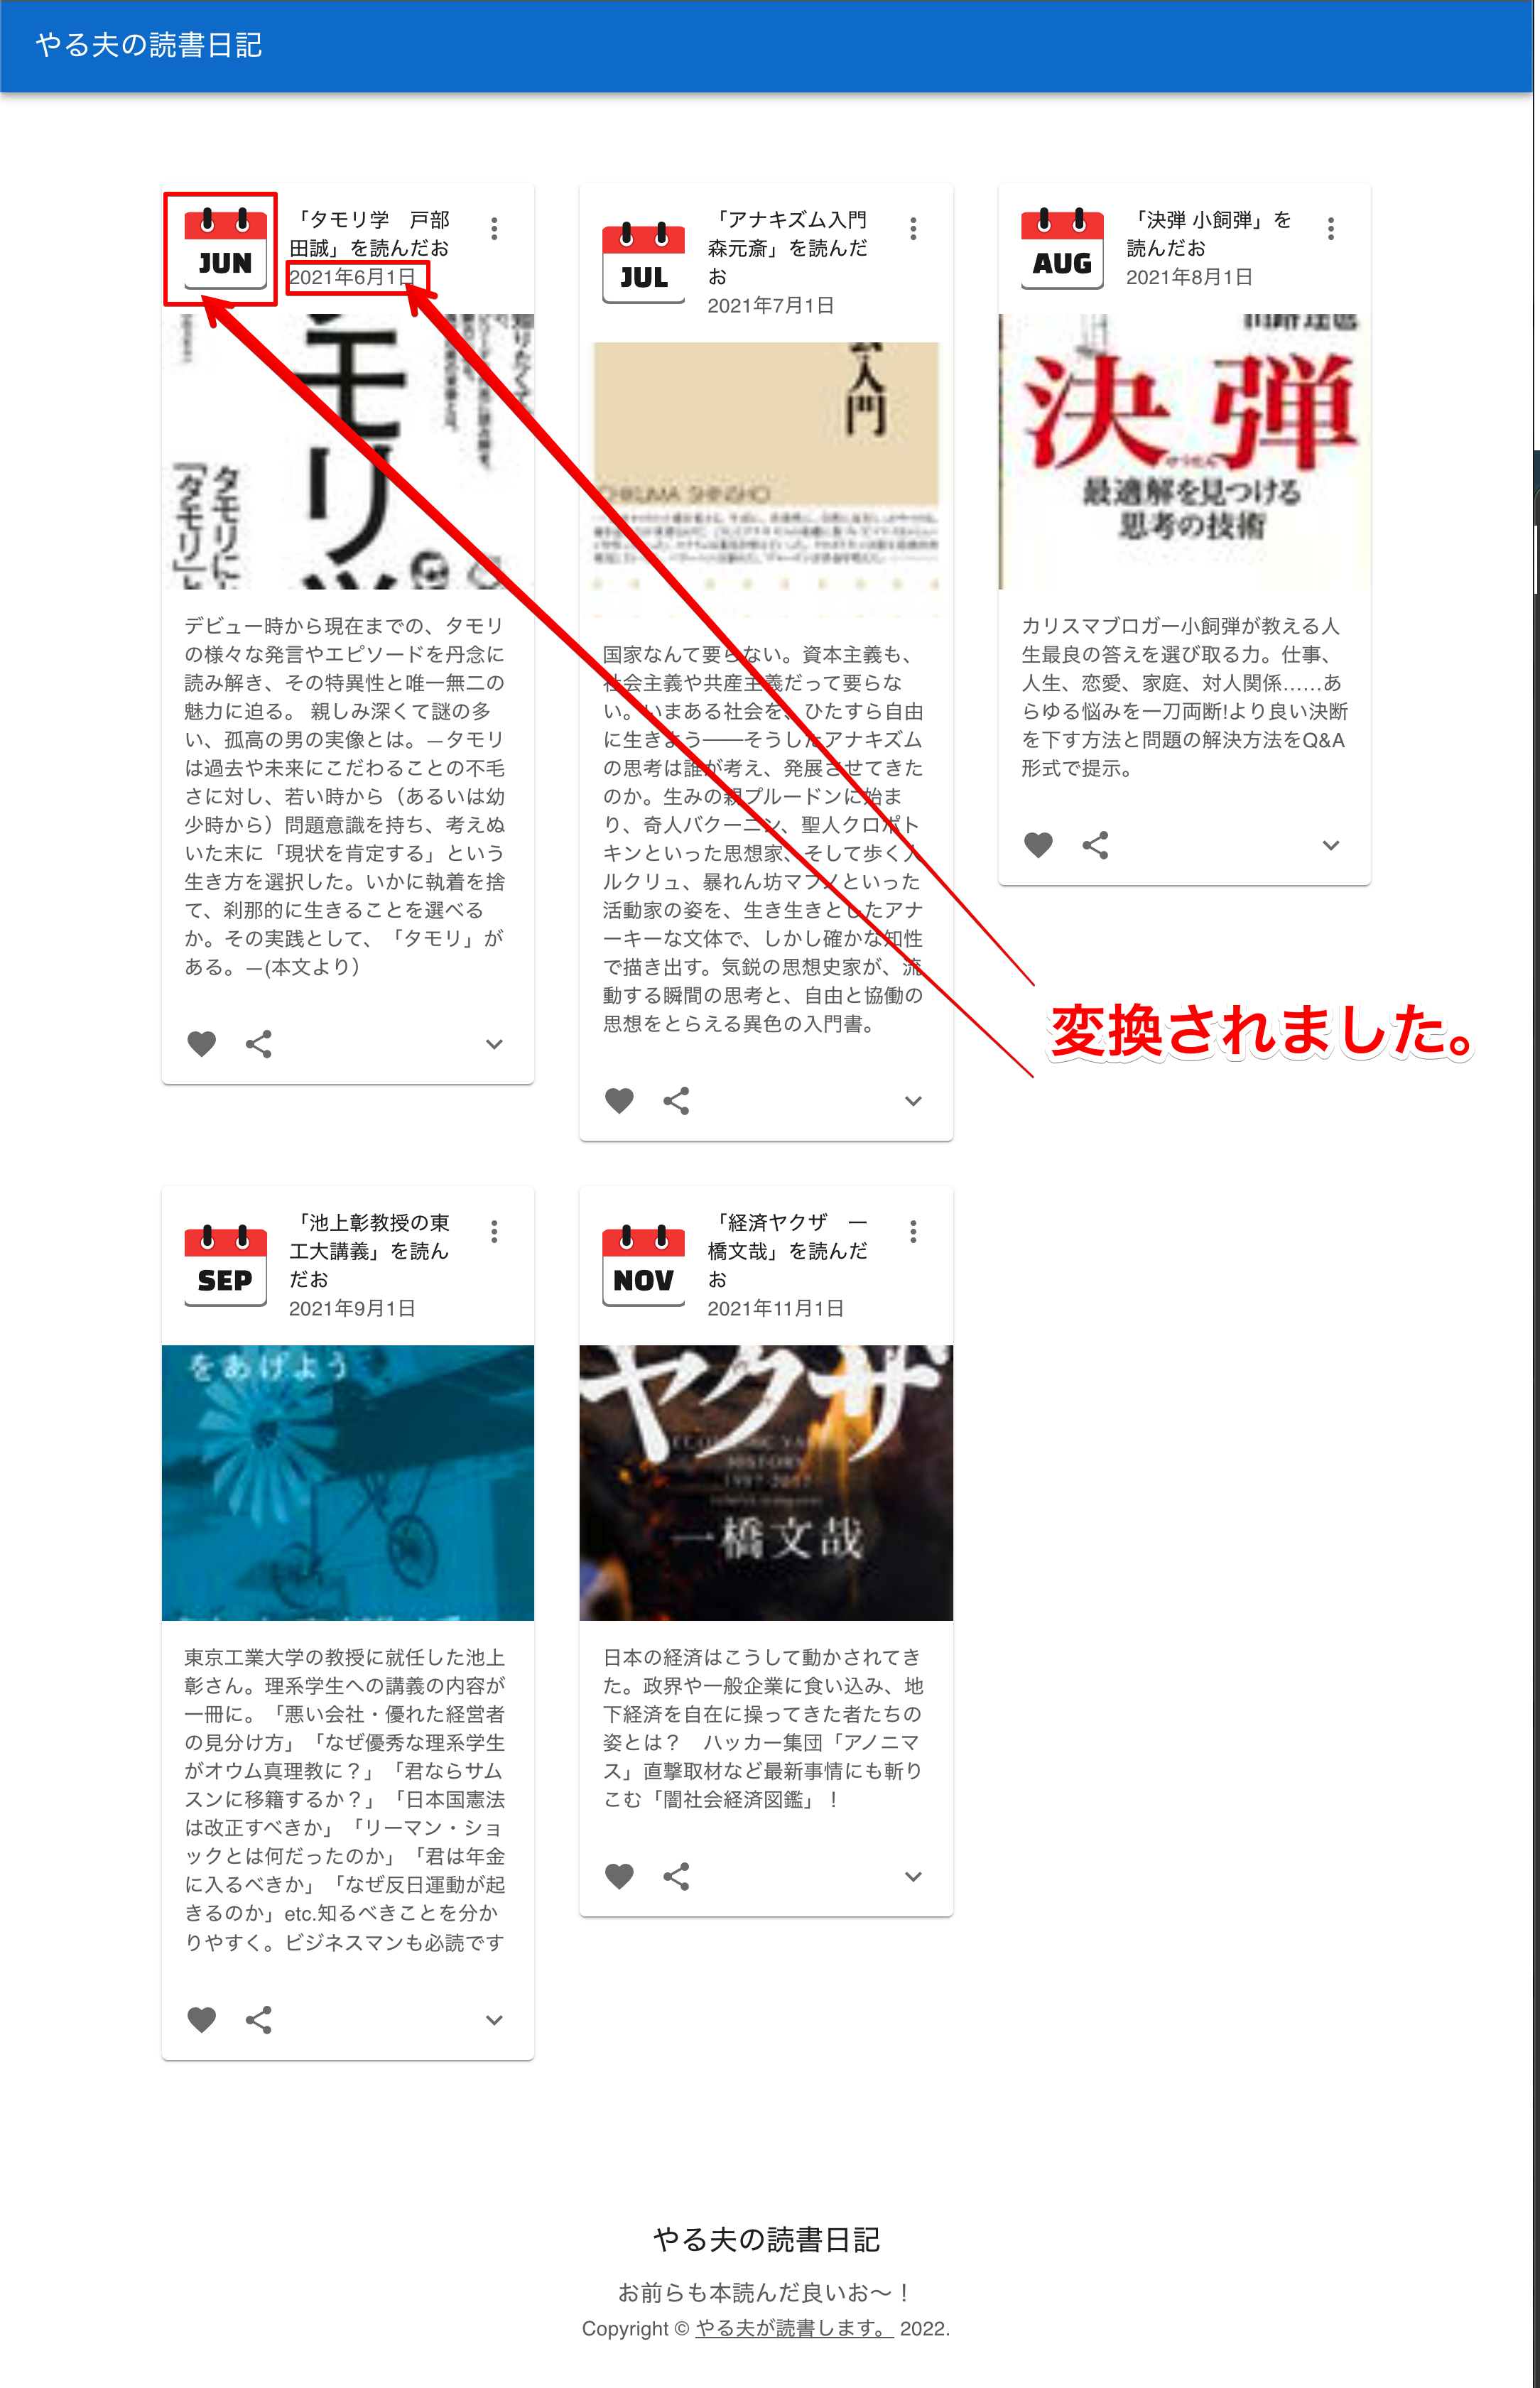
\includegraphics[width=0.7\maxwidth]{./images/03-todo-with-react/mui015-card-Header-done.png}%
\reviewimagecaption{desc}
\label{image:03-todo-with-react:mui015-card-Header-done}
\end{reviewimage}
\begin{starternote}[]{}

ここまでの内容は、GitHub上で、以下のコマンドでクローンできます。

\def\startercodeblockfontsize{}
\begin{starterterminal}[]{GitHub}\seqsplit{\textgreater{} git clone {-}b 04\textunderscore{}refactoring\textunderscore{}DiaryHeader https://github.com/yaruo{-}react{-}redux/yaruo{-}diary.git}\end{starterterminal}
\end{starternote}

\subsection{入力フォームコンポーネントの作成}
\keeplastskip{
  \label{sec:3-3-7}
  \label{sec-0337}
  \par\nobreak
}

読書データの新規追加・編集のためのフォームを作成します。

\vspace*{\baselineskip}

フォームは、DialogとしてDiaryBoadコンポーネントに追加し、DiaryBoardコンポーネントに新規追加ボタンで表示するようにします。
作成するフォームは別コンポーネントとするために「src/components/DiaryForm.tsx」ファイルを作成します。


\clearpage


MUIサイトのComponents内のText fieldコンポーネントには、フォームとして使えそうなサンプルがあります。

\begin{reviewimage}%%mui016-muisite-textField
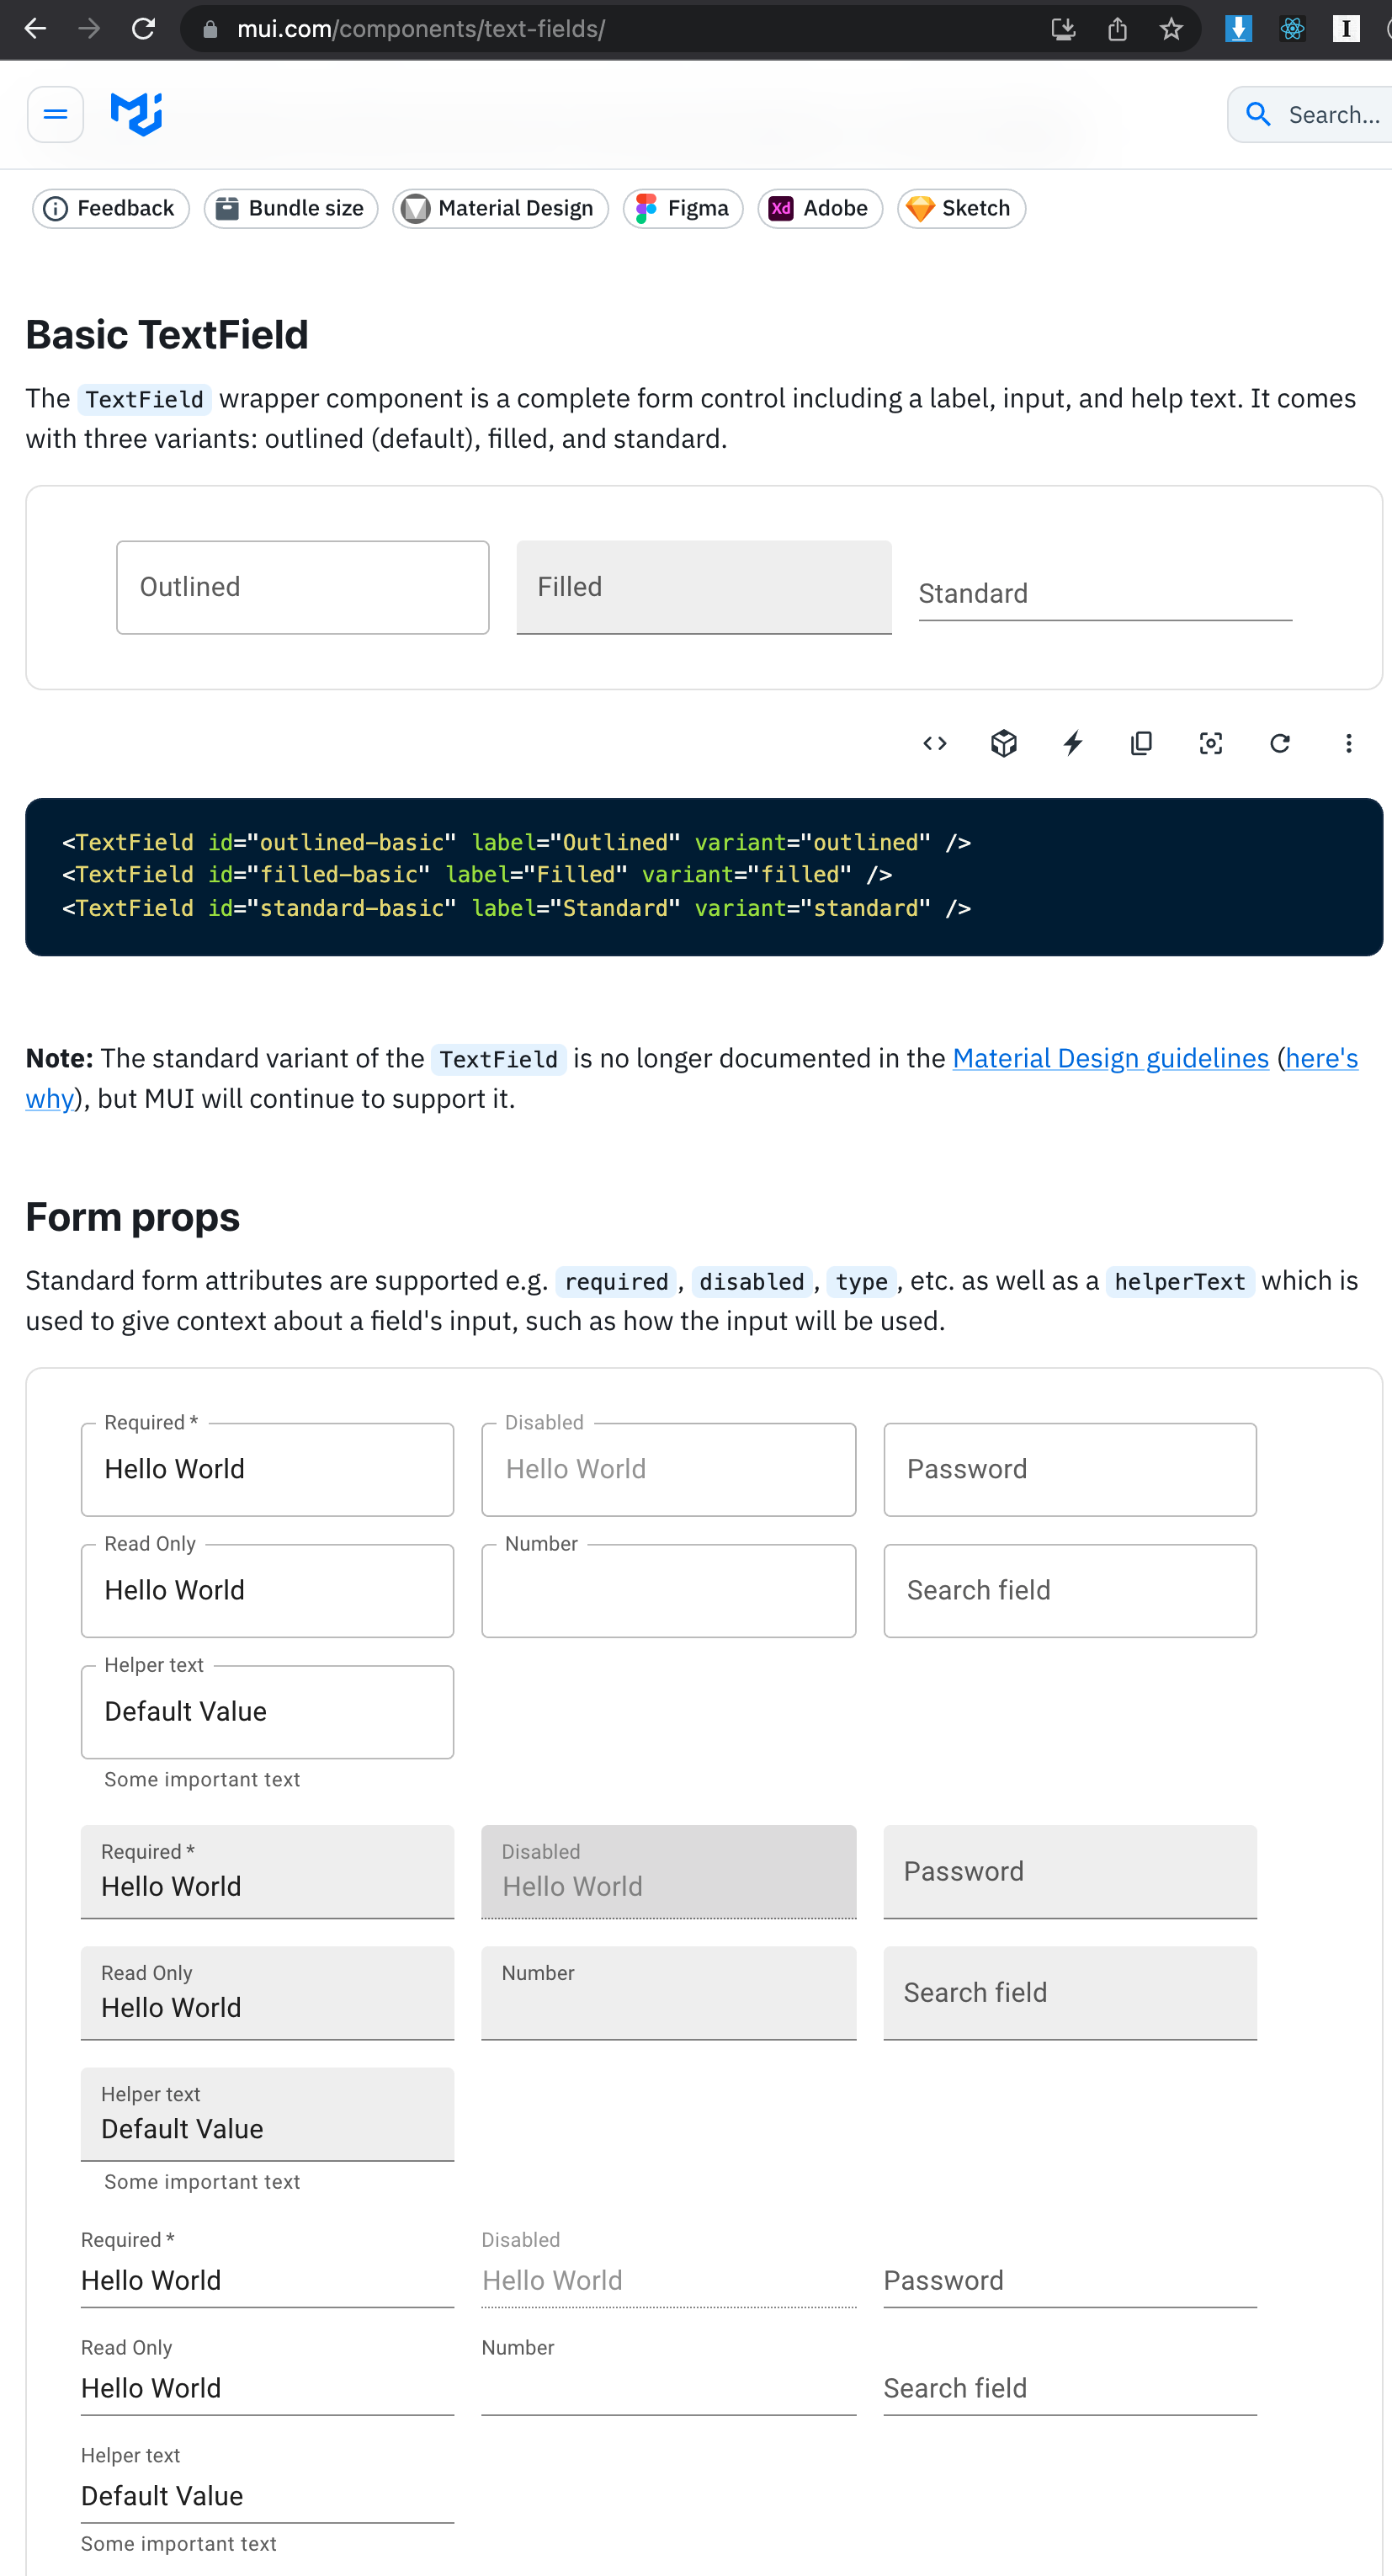
\includegraphics[width=0.6\maxwidth]{./images/03-todo-with-react/mui016-muisite-textField.png}%
\reviewimagecaption{MUIサイトのテキストフィールド}
\label{image:03-todo-with-react:mui016-muisite-textField}
\end{reviewimage}

これらを参考にしてフォームを作成します。また、投稿日の入力用にMUIのDatePickerを使うのですが、
このコンポーネントはラボ(実験中)に分類されています。そのためMUIのLabと日付を扱うためのライブラリ「date{-}fns」
をインストールします。

\begin{reviewimage}%%mui017-muisite-datePicker
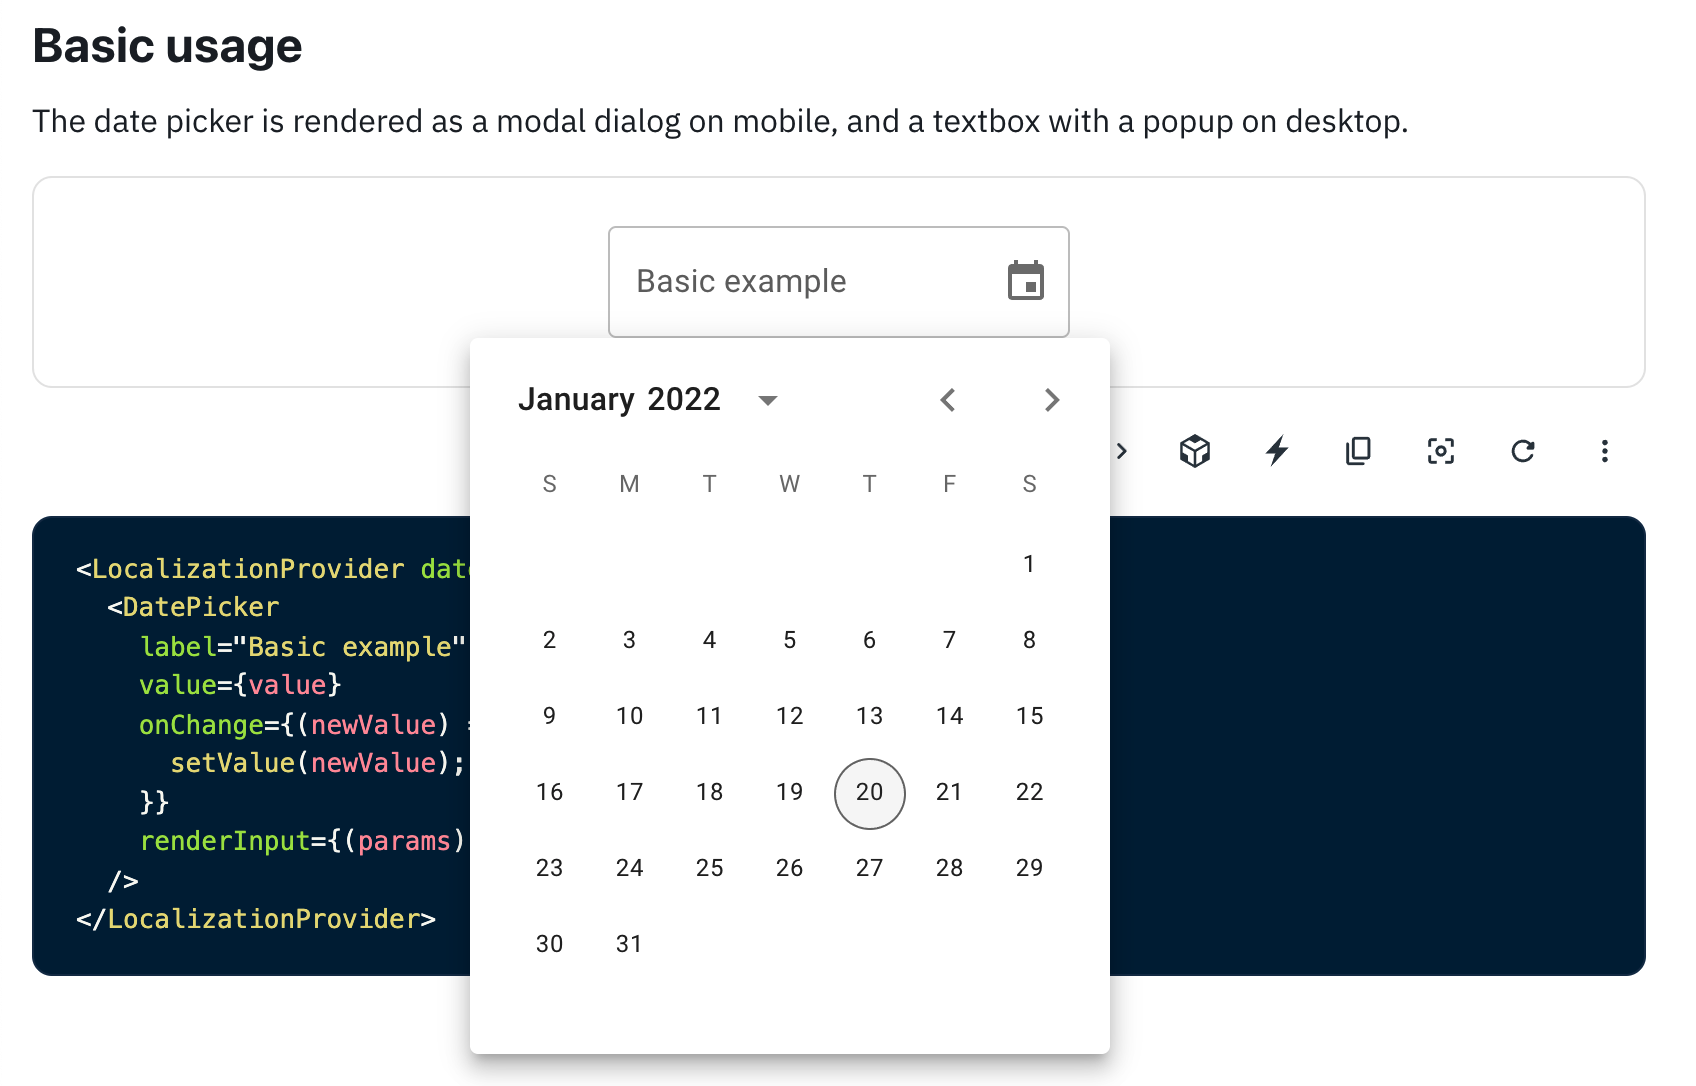
\includegraphics[width=0.7\maxwidth]{./images/03-todo-with-react/mui017-muisite-datePicker.png}%
\reviewimagecaption{MUIのDatePicker}
\label{image:03-todo-with-react:mui017-muisite-datePicker}
\end{reviewimage}
\def\startercodeblockfontsize{}
\begin{starterterminal}[]{MUIのラボ、date{-}fnsのインストール}\seqsplit{ ❯ npm install @mui/lab date{-}fns}\end{starterterminal}

DiaryFormコンポーネントは、propsとして読書日記データを受け取ります。

\begin{starteritemize}
\item 新規入力の場合には、すべてが空欄の読書日記データ
\item 編集時には、指定された読書日記データ
\end{starteritemize}

となります。

\vspace*{\baselineskip}

DiaryFormコンポーネントにあるすべてのテキストフィールドは、React HooksのひとつのuseStateを使用して
入力されたデータを保持します。

\vspace*{\baselineskip}

テキストフィールドに入力されるデータは、タイトルと本文のみは4文字以上の入力を必須とします。

作成したフォームは、こちらになります。

\def\startercodeblockfontsize{}
\begin{starterprogram}[]{DiaryForm}\seqsplit{  import React, \{ useState, useRef \} from 'react';
  import Grid from '@mui/material/Grid';
  import Paper from '@mui/material/Paper';
  import TextField from '@mui/material/TextField';
  import AdapterDateFns from '@mui/lab/AdapterDateFns';
  import LocalizationProvider from '@mui/lab/LocalizationProvider';
  import DatePicker from '@mui/lab/DatePicker';
  import Button from '@mui/material/Button';
  import CancelIcon from '@mui/icons{-}material/Cancel';
  import DataSaverOnIcon from '@mui/icons{-}material/DataSaverOn';
  import Stack from '@mui/material/Stack';

  import \{ convertStringToDate \} from '../utilities/helper';
  import \{ Diary \} from '../diaryData';

  interface DiaryFormProps \{
    diary: Diary;
  \}

  const DiaryForm = (props: DiaryFormProps) =\textgreater{} \{
    const \{ diary \} = props;
    const \{
      diaryId,
      title,
      postDate,
      imageUrl,
      imageLabel,
      mainContent,
      readmore,
    \} = diary;

    // hooksでフォームデータ保持
    // タイトル
    const [onEditTitle, setOnEditTitle] = useState(title);
    const [diaryTitleErr, setDiaryTitleErr] = useState(false);
    const [diaryTitleErrMsg, setDiaryTitleErrMsg] = useState('');
    // 投稿日
    const [onEditPostDate, setOnEditPostDate] = useState\textless{}Date \textbar{} null\textgreater{}(
      convertStringToDate(postDate)
    );
    // 画像URL
    const [onEditImageUrl, setOnEditImageUrl] = useState(imageUrl);
    // 画像ALT
    const [onEditImageLabel, setOnEditImageLabel] = useState(imageLabel);
    // 本文
    const [onEditMainContent, setOnEditMainContent] = useState(mainContent);
    const [mainContentErr, setMainContentErr] = useState(false);
    const [mainContentErrMsg, setMainContentErrMsg] = useState('');
    // 追記
    const [onEditReadMore, setOnEditReadMore] = useState(readmore.join('\reviewbackslash{}n\reviewbackslash{}n'));

    const titleRef = useRef\textless{}HTMLInputElement\textgreater{}(null);
    const mainContentRef = useRef\textless{}HTMLInputElement\textgreater{}(null);

    // 入力データ検証
    const validateFieldData = (event: React.ChangeEvent\textless{}HTMLInputElement\textgreater{}) =\textgreater{} \{
      switch (event.target.name) \{
        case 'diaryTitle':
          setOnEditTitle(event.target.value);
          if (event.target.value.length \textless{} 5) \{
            setDiaryTitleErr(true);
            setDiaryTitleErrMsg('4文字以上入力してください。');
          \} else \{
            setDiaryTitleErr(false);
            setDiaryTitleErrMsg('');
          \}
          break;
        case 'diaryMainContent':
          setOnEditMainContent(event.target.value);
          if (event.target.value.length \textless{} 5) \{
            setMainContentErr(true);
            setMainContentErrMsg('4文字以上入力してください。');
          \} else \{
            setMainContentErr(false);
            setMainContentErrMsg('');
          \}
          break;
        case 'diaryReadMore':
          setOnEditReadMore(event.target.value);
          break;
        case 'diaryImageUrl':
          setOnEditImageUrl(event.target.value);
          break;
        case 'diaryImageLabel':
          setOnEditImageLabel(event.target.value);
          break;
        default:
          break;
      \}
    \};

    // 保存ボタン
    const saveData = () =\textgreater{} \{\};

    // キャンセルボタン
    const cancelForm = () =\textgreater{} \{\};

    return (
      \textless{}Paper variant='outlined' sx=\{\{ m: 1, py: 2 \}\}\textgreater{}
        \textless{}Grid container spacing=\{2\} sx=\{\{ pl: 5 \}\}\textgreater{}
          \textless{}Grid item xs=\{10\} sm=\{10\} md=\{10\} lg=\{10\}\textgreater{}
            \textless{}TextField
              required
              id='diary{-}title'
              label='タイトル'
              error=\{diaryTitleErr\}
              fullWidth
              name='diaryTitle'
              value=\{onEditTitle\}
              helperText=\{diaryTitleErrMsg\}
              onChange=\{validateFieldData\}
              inputRef=\{titleRef\}
            /\textgreater{}
          \textless{}/Grid\textgreater{}
          \textless{}Grid item xs=\{10\} sm=\{8\} md=\{6\} lg=\{4\}\textgreater{}
            \{/* eslint{-}disable{-}next{-}line @typescript{-}eslint/no{-}unsafe{-}assignment */\}
            \textless{}LocalizationProvider dateAdapter=\{AdapterDateFns\}\textgreater{}
              \textless{}DatePicker
                label='日付'
                value=\{onEditPostDate\}
                onChange=\{(newValue: Date \textbar{} null) =\textgreater{} \{
                  setOnEditPostDate(newValue);
                \}\}
                // eslint{-}disable{-}next{-}line react/jsx{-}props{-}no{-}spreading
                renderInput=\{(params) =\textgreater{} \textless{}TextField \{...params\} /\textgreater{}\}
              /\textgreater{}
            \textless{}/LocalizationProvider\textgreater{}
          \textless{}/Grid\textgreater{}
          \textless{}Grid item xs=\{10\} sm=\{10\} md=\{10\} lg=\{10\}\textgreater{}
            \textless{}TextField
              required
              multiline
              id='diary{-}mainContent'
              label='本文'
              error=\{mainContentErr\}
              fullWidth
              name='diaryMainContent'
              value=\{onEditMainContent\}
              helperText=\{mainContentErrMsg\}
              onChange=\{validateFieldData\}
              inputRef=\{mainContentRef\}
            /\textgreater{}
          \textless{}/Grid\textgreater{}
          \textless{}Grid item xs=\{10\} sm=\{10\} md=\{10\} lg=\{10\}\textgreater{}
            \textless{}TextField
              multiline
              minRows='4'
              maxRows='6'
              id='diary{-}readmore'
              label='追記'
              fullWidth
              name='diaryReadMore'
              value=\{onEditReadMore\}
              onChange=\{validateFieldData\}
              helperText='空行を入れると段落表示されます。'
            /\textgreater{}
          \textless{}/Grid\textgreater{}
          \textless{}Grid item xs=\{10\} sm=\{10\} md=\{10\} lg=\{10\}\textgreater{}
            \textless{}TextField
              id='diary{-}imageUrl'
              label='画像URL'
              fullWidth
              name='diaryImageUrl'
              onChange=\{validateFieldData\}
              value=\{onEditImageUrl\}
              helperText='画像のURL'
            /\textgreater{}
          \textless{}/Grid\textgreater{}
          \textless{}Grid item xs=\{10\} sm=\{10\} md=\{10\} lg=\{10\}\textgreater{}
            \textless{}TextField
              id='diary{-}imageLabel'
              label='画像の代替テキスト'
              fullWidth
              name='diaryImageLabel'
              onChange=\{validateFieldData\}
              value=\{onEditImageLabel\}
              helperText='画像が表示されない場合のテキスト'
            /\textgreater{}
          \textless{}/Grid\textgreater{}
          \textless{}Grid item xs=\{10\} sm=\{10\} md=\{10\} lg=\{10\}\textgreater{}
            \textless{}Stack direction='row' spacing=\{2\}\textgreater{}
              \textless{}Button
                variant='contained'
                startIcon=\{\textless{}CancelIcon /\textgreater{}\}
                onClick=\{cancelForm\}
              \textgreater{}
                キャンセル
              \textless{}/Button\textgreater{}
              \textless{}Button
                variant='contained'
                endIcon=\{\textless{}DataSaverOnIcon /\textgreater{}\}
                onClick=\{saveData\}
              \textgreater{}
                保存
              \textless{}/Button\textgreater{}
            \textless{}/Stack\textgreater{}
          \textless{}/Grid\textgreater{}
        \textless{}/Grid\textgreater{}
      \textless{}/Paper\textgreater{}
    );
  \};

  export default DiaryForm;
}\end{starterprogram}

作成したフォームをダイアログとして表示するコンポーネントを作成します。

\vspace*{\baselineskip}

「src/components/DiaryFormDialog.tsx」ファイルを作成し、MUIのダイアログの表示・非表示を実装します。

\def\startercodeblockfontsize{}
\begin{starterprogram}[]{DiaryFormDialog}\seqsplit{  import React from 'react';
  import Dialog from '@mui/material/Dialog';
  import DialogTitle from '@mui/material/DialogTitle';

  import \{ Diary \} from '../diaryData';
  import DiaryForm from './DiaryForm';

  export interface DialogDiaryFormProps \{
    open: boolean;
    diary: Diary;
  \}

  const DialogDiaryForm = (props: DialogDiaryFormProps) =\textgreater{} \{
    const \{ open, diary \} = props;

    return (
      \textless{}Dialog open=\{open\}\textgreater{}
        \textless{}DialogTitle\textgreater{}日記編集\textless{}/DialogTitle\textgreater{}
        \textless{}DiaryForm diary=\{diary\} /\textgreater{}
      \textless{}/Dialog\textgreater{}
    );
  \};

  export default DialogDiaryForm;}\end{starterprogram}

DiaryBoardコンポーネントに、新規追加ボタン追加しフォームが開くよう実装します。

\begin{starterenumerate}
\item 空欄の初期化データinitialDiaryを作成
\item DiaryFormDialogコンポーネントをインポートし追加
\item 新規追加アイコンをツールバーに追加し、クリックするとDiaryFormDialogが開く
\end{starterenumerate}

以上の変更を加えた「DiaryBoardコンポーネント」は、こちらになります。

\def\startercodeblockfontsize{}
\begin{starterprogram}[]{新規追加ボタンを追加したDiaryBoardコンポーネント}\seqsplit{  import React, \{ useState \} from 'react';
  import AppBar from '@mui/material/AppBar';
  import Grid from '@mui/material/Grid';
  import Box from '@mui/material/Box';
  import Toolbar from '@mui/material/Toolbar';
  import Typography from '@mui/material/Typography';
  import Container from '@mui/material/Container';
  import Link from '@mui/material/Link';
  import IconButton from '@mui/material/IconButton';
  import AddCircleOutlineIcon from '@mui/icons{-}material/AddCircleOutline';

  import \{ Diary \} from '../diaryData';
  import DiaryCard from './DiaryCard';
  import DiaryFormDialog from './DiaryFormDialog';

  export type DiaryBoardProps = \{
    diaries: Diary[];
  \};

  // diary初期化データ
  const initialDiary: Diary = \{
    diaryId: '',
    title: '',
    postDate: '',
    imageUrl: '',
    imageLabel: '',
    mainContent: '',
    readmore: [],
  \};

  const Copyright = () =\textgreater{} (
    \textless{}Typography variant='body2' color='text.secondary' align='center'\textgreater{}
      \{'Copyright © '\}
      \textless{}Link color='inherit' href='https://mui.com/'\textgreater{}
        やる夫が読書します。
      \textless{}/Link\textgreater{}
      \{` \textdollar{}\{new Date().getFullYear()\}.`\}
    \textless{}/Typography\textgreater{}
  );

  const DiaryBoard = (props: DiaryBoardProps) =\textgreater{} \{
    const \{ diaries \} = props;

    // DiaryFormDialogの開閉状態
    const [openDialog, setOpenDialog] = useState(false);

    // 新規データでDiaryFormDialogを開く
    const openForm = () =\textgreater{} setOpenDialog(true);

    return (
      \textless{}\textgreater{}
        \textless{}AppBar position='relative'\textgreater{}
          \textless{}Toolbar\textgreater{}
            \textless{}Box sx=\{\{ flexGrow: 1 \}\}\textgreater{}
              \textless{}Typography variant='h6' color='inherit' noWrap\textgreater{}
                やる夫の読書日記
              \textless{}/Typography\textgreater{}
            \textless{}/Box\textgreater{}
            \textless{}Box\textgreater{}
              \textless{}IconButton
                size='large'
                edge='end'
                aria{-}label='新規読書日記'
                onClick=\{openForm\}
                color='inherit'
              \textgreater{}
                \textless{}AddCircleOutlineIcon /\textgreater{}
              \textless{}/IconButton\textgreater{}
            \textless{}/Box\textgreater{}
          \textless{}/Toolbar\textgreater{}
        \textless{}/AppBar\textgreater{}
        \textless{}main\textgreater{}
          \textless{}Container sx=\{\{ py: 8 \}\} maxWidth='md'\textgreater{}
            \textless{}Grid container spacing=\{4\}\textgreater{}
              \{diaries.map((diary) =\textgreater{} (
                \textless{}Grid item key=\{diary.diaryId\} xs=\{12\} sm=\{6\} md=\{4\}\textgreater{}
                  \textless{}DiaryCard diary=\{diary\} /\textgreater{}
                \textless{}/Grid\textgreater{}
              ))\}
            \textless{}/Grid\textgreater{}
          \textless{}/Container\textgreater{}
        \textless{}/main\textgreater{}
        \{/* Footer */\}
        \textless{}Box sx=\{\{ bgcolor: 'background.paper', p: 6 \}\} component='footer'\textgreater{}
          \textless{}Typography variant='h6' align='center' gutterBottom\textgreater{}
            やる夫の読書日記
          \textless{}/Typography\textgreater{}
          \textless{}Typography
            variant='subtitle1'
            align='center'
            color='text.secondary'
            component='p'
          \textgreater{}
            お前らも本読んだ良いお〜!
          \textless{}/Typography\textgreater{}
          \textless{}Copyright /\textgreater{}
        \textless{}/Box\textgreater{}
        \{/* End footer */\}
        \textless{}DiaryFormDialog open=\{openDialog\} diary=\{initialDiary\} /\textgreater{}
      \textless{}/\textgreater{}
    );
  \};

  export default DiaryBoard;
}\end{starterprogram}

変更が完了したら動作確認をします。ツールバーに「+」のアイコンボタンが表示され、クリックすると入力フォームが開きます。

\begin{starteritemize}
\item それぞれのテキストフィールドに入力はできますか?
\item タイトルと本文が4文字以下だとエラーがでますか?
\item DatePickerは、動作しますか?
\end{starteritemize}

開いた入力フォームですが、保存・キャンセルとも機能実装していません。そのため一度開いたフォームを閉じることができません。


\clearpage

\begin{reviewimage}%%mui018-DiaryForm-done
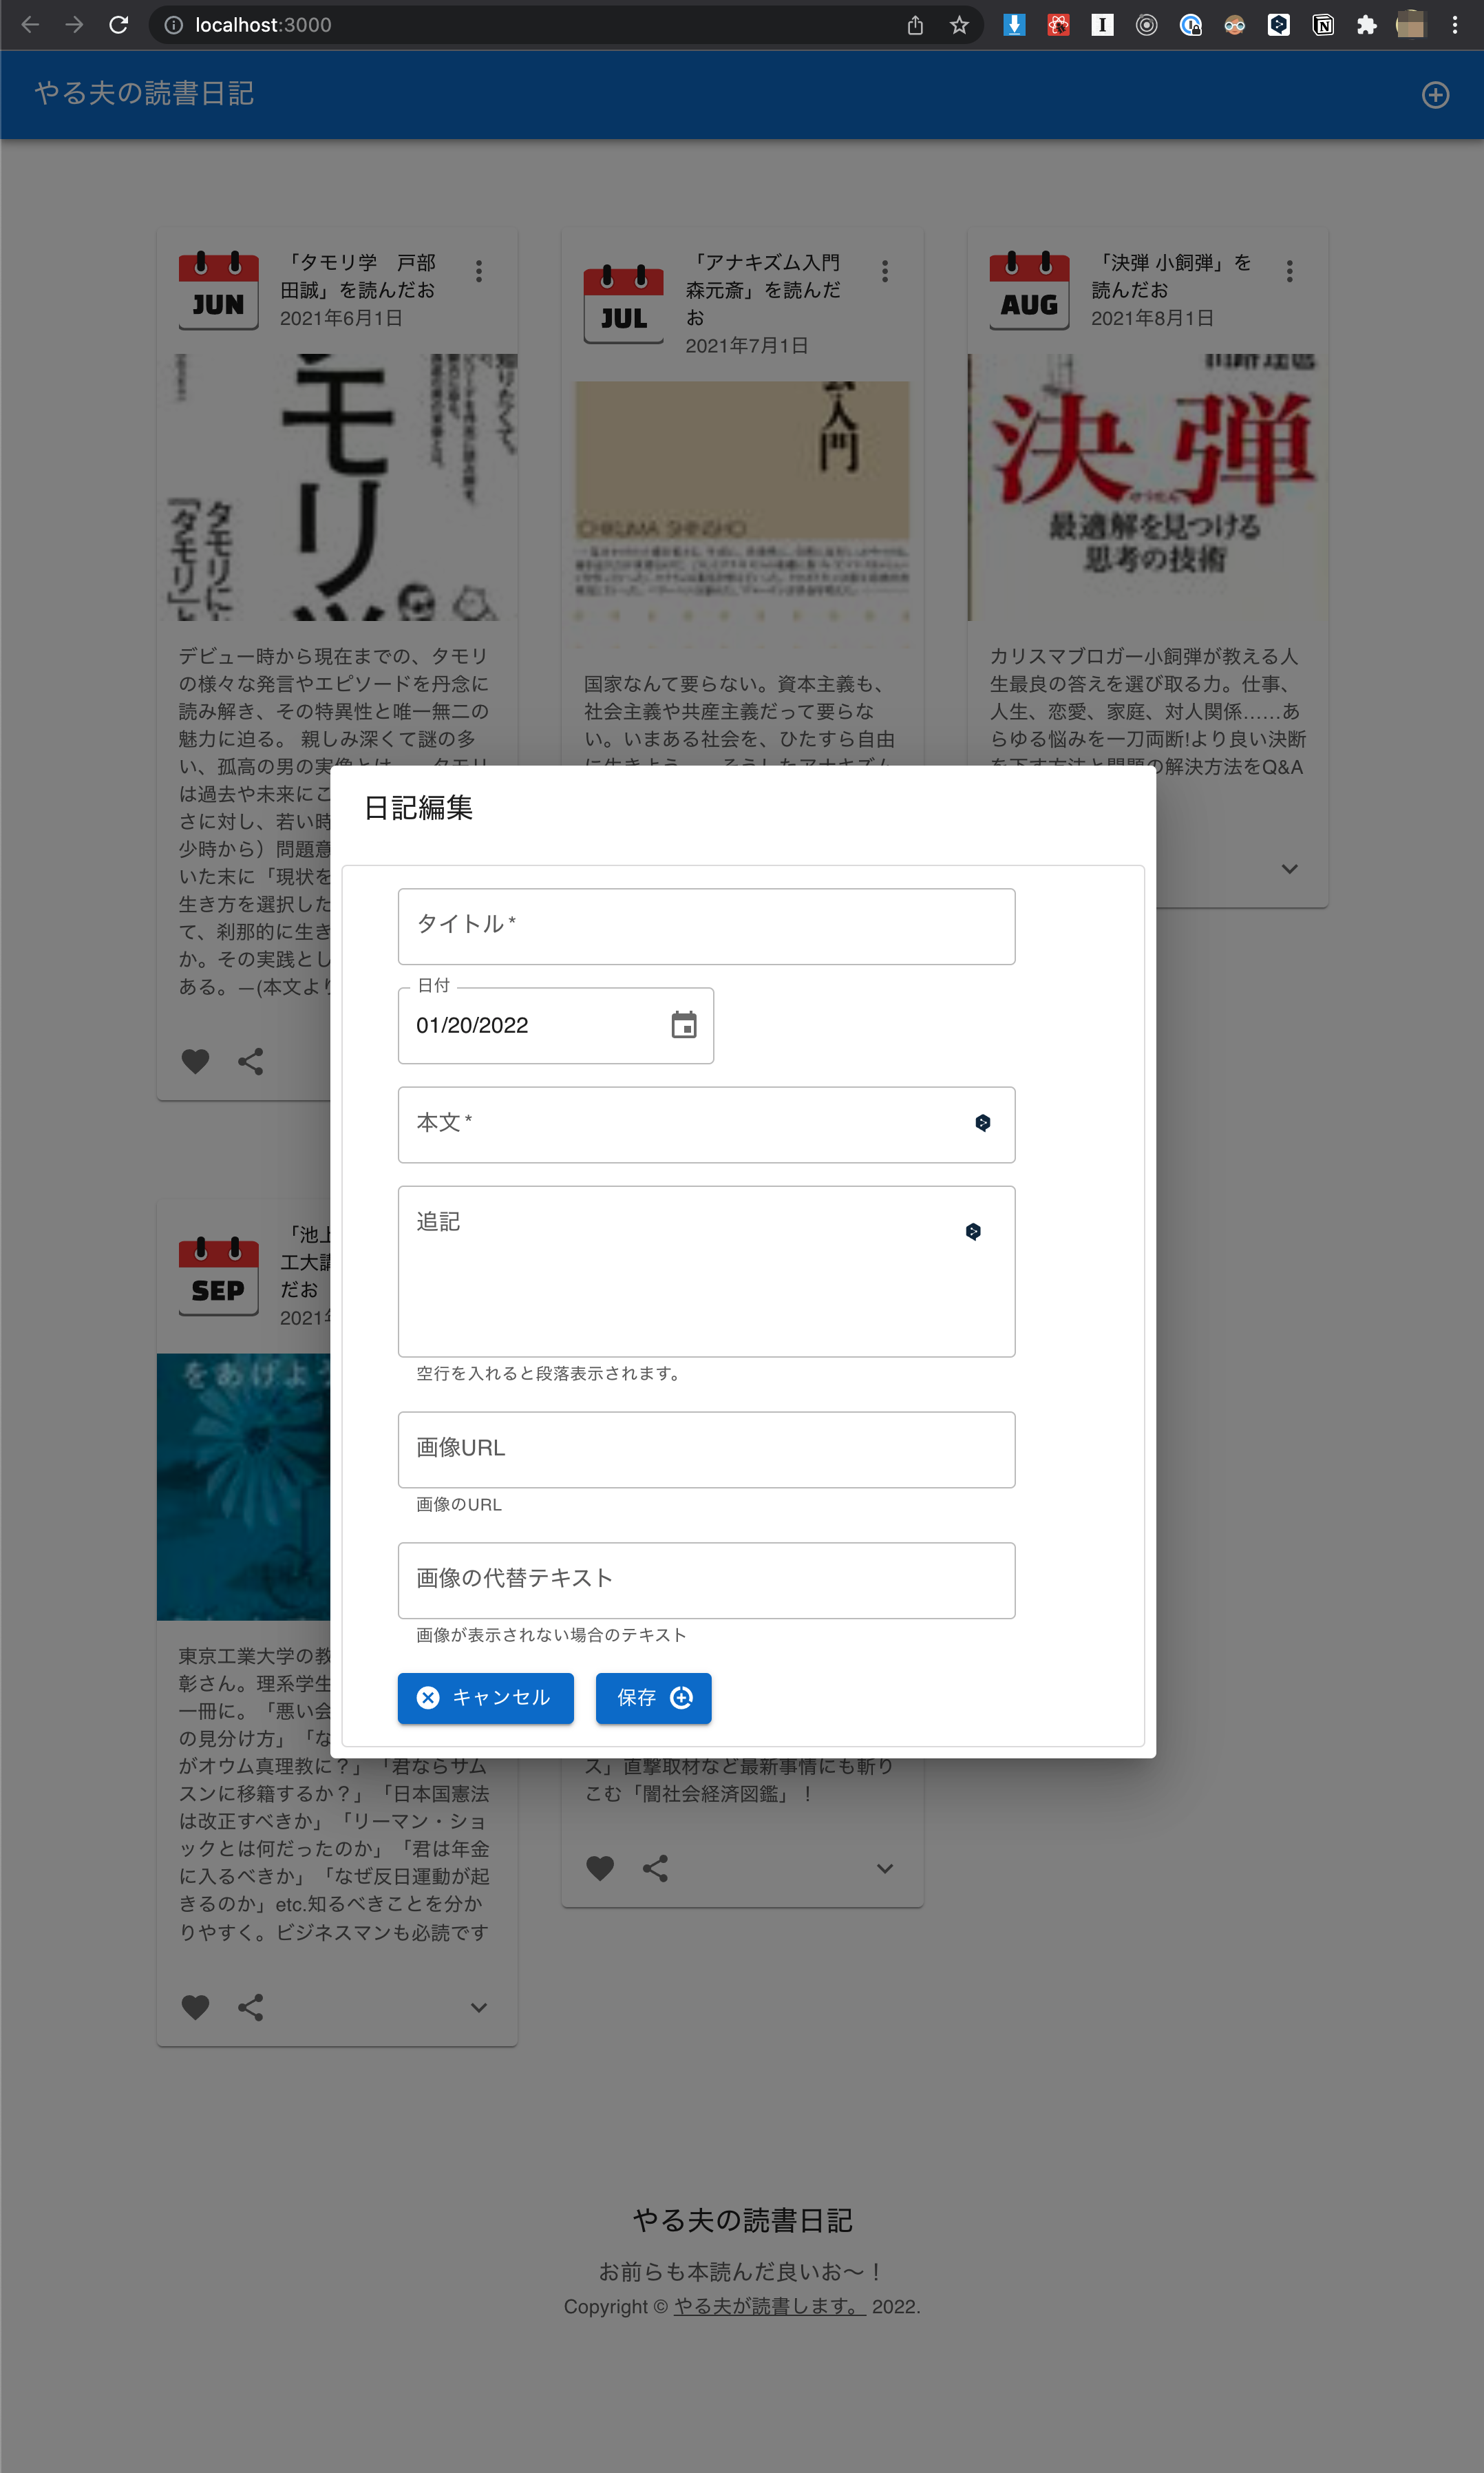
\includegraphics[width=0.7\maxwidth]{./images/03-todo-with-react/mui018-DiaryForm-done.png}%
\reviewimagecaption{入力フォームを開いた状態}
\label{image:03-todo-with-react:mui018-DiaryForm-done}
\end{reviewimage}

\section{データの追加・編集・削除}
\keeplastskip{
  \label{sec:3-4}
  \label{sec-034hooks}
  \par\nobreak
}

表示用のコンポーネントが完成したので、データの追加・編集削除ができるように機能実装を行います。

\vspace*{\baselineskip}

分かりづらい図ですが、コンポーネントの構成を図にしました。
Reactコンポーネントは表示するためのデータをPropsを介して受け取るため、孫コンポーネントに表示するデータも
祖父母コンポーネントから親コンポーネントを経由して渡します。

\vspace*{\baselineskip}

これが「Reactあるある」のひとつの「Propsバケツリレー」です。

\begin{reviewimage}%%AppComponents
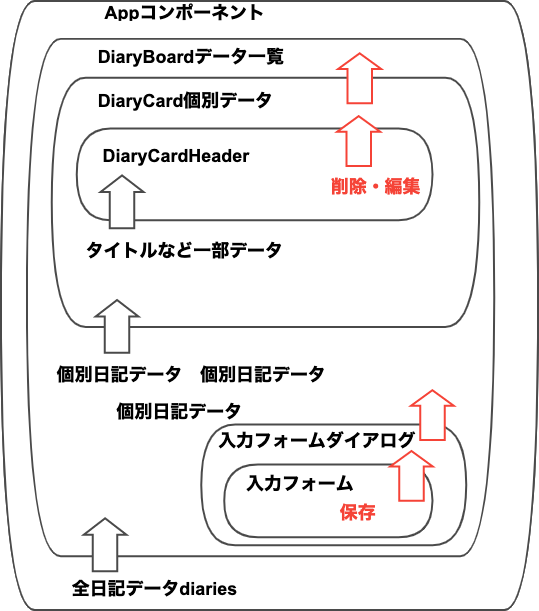
\includegraphics[width=1.0\maxwidth]{./images/03-todo-with-react/AppComponents.png}%
\reviewimagecaption{コンポーネントの構成図}
\label{image:03-todo-with-react:AppComponents}
\end{reviewimage}

今回のように孫コンポーネントにあたる「DiaryCardHeaderコンポーネント」の編集・削除の要求があった場合には
全データを管理する「DiaryBoadコンポーネント」に伝えなければなりません。

\vspace*{\baselineskip}

表示は、親コンポーネントからバケツリレーで伝え、
孫コンポーネントで受けたユーザーからの要求は逆のルートをたどって親まで伝えなければなりません。
孫で発生した要求を親に伝える方法として一般的なのが、関数をPropsとしてデータと伴に子・孫へ渡す方法です。

\vspace*{\baselineskip}

今回のアプリケーションでは、DiaryBoadコンポーネントが、

\begin{starteritemize}
\item 削除要求は、diaryIdを知らせてね。
\item 編集要求は、全データ持っているので編集対象のdiaryIdを知らせてね。フォームにセットするから。
\item 入力フォームでの保存要求は、保存するデータをください。diaryIdが既存のものは上書き、ほかは追加。
\end{starteritemize}

の関数をそれぞれのコンポーネントにバケツリレーし、孫で関数を実行すれば親に要求が伝わることになります。

\vspace*{\baselineskip}

データの変化が起こると、ブラウザが再描画されます。Reactコンポーネントの場合、
再描画されるためのデータの変化とは、propsとコンポーネント自身で管理しているものです。

\vspace*{\baselineskip}

DiaryBoadコンポーネントでは、管理するデータをuseStateで状態管理し、ブラウザの描画にもその状態を使う
必要があります。そのためDiaryBoadコンポーネントにuseStateを追加します。

\def\startercodeblockfontsize{}
\begin{starterprogram}[]{DiaryBoad.tsx}\seqsplit{  // 全データ Appコンポーネントから受け取ったデータで初期化する
  const [diaryData, setDiaryData] = useState(diaries);

・・・中略

 // 管理しているデータを描画に使用する
  \textless{}Grid container spacing=\{4\}\textgreater{}
    \{diaryData.map((diary) =\textgreater{} (
      \textless{}Grid item key=\{diary.diaryId\} xs=\{12\} sm=\{6\} md=\{4\}\textgreater{}
        \textless{}DiaryCard
          diary=\{diary\}
          onClickCardHeaderAction=\{onClickCardHeaderAction\}
        /\textgreater{}
      \textless{}/Grid\textgreater{}
    ))\}
  \textless{}/Grid\textgreater{}}\end{starterprogram}

\subsection{削除・編集関数をPropsにデータと渡す}
\keeplastskip{
  \label{sec:3-4-1}
  \label{sec-034-1}
  \par\nobreak
}

DiaryCardHeaderコンポーネントのPropsに「diaryId、編集・削除フラグ」を引数とする関数を追加します。

\def\startercodeblockfontsize{}
\begin{starterterminal}[]{DiaryCardHeader.tsxの変更}\seqsplit{  export type DiaryCardHeaderProps = \{
    diaryId: string;
    title: string;
    postDate: string;
    onClickCardHeaderAction: (diaryId: string, mode: string) =\textgreater{} void;
  \};}\end{starterterminal}

DiaryHeaderコンポーネントでは、受けたPropsから関数を取り出し、メニューがクリックされたときに
実行する関数を実装します。

\def\startercodeblockfontsize{}
\begin{starterprogram}[]{DiaryCardHeader.tsx}\seqsplit{  //propsからの取り出し
  const \{ onClickCardHeaderAction, diaryId, title, postDate \} = props;

  // 編集メニュークリック
  const handleEdit = () =\textgreater{} \{
    handleCloseMenu();
    return onClickCardHeaderAction(diaryId, 'EDIT');
  \};

  // ダイアログの削除ボタンクリック
  const handleConfirmDelete = () =\textgreater{} \{
    setOpenDialog(false);
    return onClickCardHeaderAction(diaryId, 'DELETE');
  \};
}\end{starterprogram}

完成したDiaryCardHeaderコンポーネントは、こちらです。

\def\startercodeblockfontsize{}
\begin{starterprogram}[]{DiaryCardHeader.tsx}\seqsplit{  /* eslint{-}disable @typescript{-}eslint/no{-}unsafe{-}assignment */
  import React from 'react';
  import CardHeader from '@mui/material/CardHeader';
  import Avatar from '@mui/material/Avatar';
  import Menu from '@mui/material/Menu';
  import MenuItem from '@mui/material/MenuItem';
  import ListItemIcon from '@mui/material/ListItemIcon';
  import MoreVertIcon from '@mui/icons{-}material/MoreVert';
  import EditIcon from '@mui/icons{-}material/Edit';
  import DeleteForeverIcon from '@mui/icons{-}material/DeleteForever';
  import IconButton from '@mui/material/IconButton';
  import Button from '@mui/material/Button';
  import Dialog from '@mui/material/Dialog';
  import DialogActions from '@mui/material/DialogActions';
  import DialogContent from '@mui/material/DialogContent';
  import DialogContentText from '@mui/material/DialogContentText';
  import DialogTitle from '@mui/material/DialogTitle';

  import January from '../assets/images/month{-}icons/january.svg';
  import February from '../assets/images/month{-}icons/february.svg';
  import March from '../assets/images/month{-}icons/march.svg';
  import April from '../assets/images/month{-}icons/april.svg';
  import May from '../assets/images/month{-}icons/may.svg';
  import Jun from '../assets/images/month{-}icons/june.svg';
  import July from '../assets/images/month{-}icons/july.svg';
  import August from '../assets/images/month{-}icons/august.svg';
  import September from '../assets/images/month{-}icons/september.svg';
  import October from '../assets/images/month{-}icons/october.svg';
  import November from '../assets/images/month{-}icons/november.svg';
  import December from '../assets/images/month{-}icons/december.svg';

  import \{
    convertToLongDateString,
    convertStringToDate,
  \} from '../utilities/helper';

  export type DiaryCardHeaderProps = \{
    diaryId: string;
    title: string;
    postDate: string;
    onClickCardHeaderAction: (diaryId: string, mode: string) =\textgreater{} void;
  \};

  const DiaryCardHeader = (props: DiaryCardHeaderProps) =\textgreater{} \{
    const \{ onClickCardHeaderAction, diaryId, title, postDate \} = props;

    // menuの開閉状態を管理
    const [anchorEl, setAnchorEl] = React.useState\textless{}null \textbar{} HTMLElement\textgreater{}(null);
    // ダイアログの表示・非表示
    const [openDialog, setOpenDialog] = React.useState(false);

    // menuの開閉
    const openMenu = Boolean(anchorEl);
    // MoreVerIconクリック
    const handleClick = (event: React.MouseEvent\textless{}HTMLElement\textgreater{}) =\textgreater{} \{
      setAnchorEl(event.currentTarget);
    \};

    // menuを閉じる
    const handleCloseMenu = () =\textgreater{} \{
      setAnchorEl(null);
    \};

    // ダイアログ表示
    const handleClickOpenDialog = () =\textgreater{} \{
      handleCloseMenu();
      setOpenDialog(true);
    \};

    // 編集メニュークリック
    const handleEdit = () =\textgreater{} \{
      handleCloseMenu();
      return onClickCardHeaderAction(diaryId, 'EDIT');
    \};

    // 削除メニュークリック
    const handleDelete = () =\textgreater{} \{
      handleClickOpenDialog();
    \};

    // ダイアログ非表示
    const handleCloseDialog = () =\textgreater{} \{
      setOpenDialog(false);
    \};

    // ダイアログの削除ボタンクリック
    const handleConfirmDelete = () =\textgreater{} \{
      setOpenDialog(false);
      return onClickCardHeaderAction(diaryId, 'DELETE');
    \};

    // postDate:YYYYMMDDから月を取得し
    const datePosted: Date = convertStringToDate(postDate);
    let avatarSrc;
    // useEffect(() =\textgreater{} \{
    switch (datePosted.getMonth()) \{
      case 0:
        avatarSrc = January;
        break;
      case 1:
        avatarSrc = February;
        break;
      case 2:
        avatarSrc = March;
        break;
      case 3:
        avatarSrc = April;
        break;
      case 4:
        avatarSrc = May;
        break;
      case 5:
        avatarSrc = Jun;
        break;
      case 6:
        avatarSrc = July;
        break;
      case 7:
        avatarSrc = August;
        break;
      case 8:
        avatarSrc = September;
        break;
      case 9:
        avatarSrc = October;
        break;
      case 10:
        avatarSrc = November;
        break;
      case 11:
        avatarSrc = December;
        break;
      default:
        break;
    \}

    const posted = convertToLongDateString(postDate);

    return (
      \textless{}\textgreater{}
        \textless{}CardHeader
          avatar=\{
            \textless{}Avatar
              sx=\{\{ width: 58, height: 58 \}\}
              variant='square'
              aria{-}label=\{`投稿日:\textdollar{}\{posted\}`\}
              src=\{avatarSrc\}
            /\textgreater{}
          \}
          action=\{
            \textless{}IconButton aria{-}label='settings' onClick=\{handleClick\}\textgreater{}
              \textless{}MoreVertIcon /\textgreater{}
            \textless{}/IconButton\textgreater{}
          \}
          title=\{title\}
          subheader=\{posted\}
        /\textgreater{}
        \textless{}Menu
          anchorEl=\{anchorEl\}
          id='account{-}menu'
          open=\{openMenu\}
          onClose=\{handleCloseMenu\}
          onClick=\{handleCloseMenu\}
          PaperProps=\{\{
            elevation: 0,
            sx: \{
              overflow: 'visible',
              filter: 'drop{-}shadow(0px 2px 8px rgba(0,0,0,0.32))',
              mt: 1.5,
              '\& .MuiAvatar{-}root': \{
                width: 32,
                height: 32,
                ml: {-}0.5,
                mr: 1,
              \},
              '\&:before': \{
                content: '""',
                display: 'block',
                position: 'absolute',
                top: 0,
                right: 14,
                width: 10,
                height: 10,
                bgcolor: 'background.paper',
                transform: 'translateY({-}50\%) rotate(45deg)',
                zIndex: 0,
              \},
            \},
          \}\}
          transformOrigin=\{\{ horizontal: 'right', vertical: 'top' \}\}
          anchorOrigin=\{\{ horizontal: 'right', vertical: 'bottom' \}\}
        \textgreater{}
          \textless{}MenuItem onClick=\{handleEdit\}\textgreater{}
            \textless{}ListItemIcon\textgreater{}
              \textless{}EditIcon fontSize='small' /\textgreater{}
            \textless{}/ListItemIcon\textgreater{}
            編集
          \textless{}/MenuItem\textgreater{}
          \textless{}MenuItem onClick=\{handleDelete\}\textgreater{}
            \textless{}ListItemIcon\textgreater{}
              \textless{}DeleteForeverIcon fontSize='small' /\textgreater{}
            \textless{}/ListItemIcon\textgreater{}
            削除
          \textless{}/MenuItem\textgreater{}
        \textless{}/Menu\textgreater{}
        \textless{}Dialog open=\{openDialog\} onClose=\{handleCloseDialog\}\textgreater{}
          \textless{}DialogTitle\textgreater{}削除の確認だお〜\textless{}/DialogTitle\textgreater{}
          \textless{}DialogContent\textgreater{}
            \textless{}DialogContentText\textgreater{}
              削除すると、基には戻せないお〜!それでも削除するのかお〜?
            \textless{}/DialogContentText\textgreater{}
          \textless{}/DialogContent\textgreater{}
          \textless{}DialogActions\textgreater{}
            \textless{}Button onClick=\{handleCloseDialog\}\textgreater{}キャンセル\textless{}/Button\textgreater{}
            \textless{}Button onClick=\{handleConfirmDelete\}\textgreater{}削除\textless{}/Button\textgreater{}
          \textless{}/DialogActions\textgreater{}
        \textless{}/Dialog\textgreater{}
      \textless{}/\textgreater{}
    );
  \};

  export default DiaryCardHeader;
}\end{starterprogram}

次に、DiaryCardHeaderコンポーネントの親のDiaryCardコンポーネントも親から受け取り、子に渡します。

\def\startercodeblockfontsize{}
\begin{starterprogram}[]{DiaryCard.tsx}\seqsplit{  // propsの型定義
  export type DiaryCardProps = \{
    diary: Diary;
    onClickCardHeaderAction: (diaryId: string, mode: string) =\textgreater{} void;
  \};

  // DiaryCardコンポーネント
const DiaryCard = (props: DiaryCardProps) =\textgreater{} \{
  // 詳細表示コンポーネントの表示・非表示の状態
  const [expanded, setExpanded] = React.useState(false);

  // 詳細コンポーネントの表示・非表示を切り替える関数
  const handleExpandClick = () =\textgreater{} \{
    setExpanded(!expanded);
  \};

  // 受け取ったオブジェクトを変数に展開
  const \{ diary, onClickCardHeaderAction \} = props;

  return (
  \textless{}Card sx=\{\{ maxWidth: 345 \}\}\textgreater{}
    \textless{}DiaryCardHeader
      diaryId=\{diaryId\}
      title=\{title\}
      postDate=\{postDate\}
      onClickCardHeaderAction=\{onClickCardHeaderAction\} {\reviewballoon{子に送る}}
    /\textgreater{}}\end{starterprogram}

バケツリレーですので、受け取って渡すだけです。変更後のDiaryCardHeaderコンポーネントは、こうなります。

\def\startercodeblockfontsize{}
\begin{starterprogram}[]{DiaryCard.tsx}\seqsplit{  import React from 'react';
  import \{ styled \} from '@mui/material/styles';
  import Card from '@mui/material/Card';
  import CardMedia from '@mui/material/CardMedia';
  import CardContent from '@mui/material/CardContent';
  import CardActions from '@mui/material/CardActions';
  import Collapse from '@mui/material/Collapse';
  import IconButton, \{ IconButtonProps \} from '@mui/material/IconButton';
  import Typography from '@mui/material/Typography';
  import FavoriteIcon from '@mui/icons{-}material/Favorite';
  import ShareIcon from '@mui/icons{-}material/Share';
  import ExpandMoreIcon from '@mui/icons{-}material/ExpandMore';

  import \{ Diary \} from '../diaryData';
  import DiaryCardHeader from './DiaryHeader';

  export type DiaryCardProps = \{
    diary: Diary;
    onClickCardHeaderAction: (diaryId: string, mode: string) =\textgreater{} void;
  \};

  // アイコンクリックで詳細部分を表示するためのコンポーネントのpros型
  interface ExpandMoreProps extends IconButtonProps \{
    expand: boolean;
  \}

  // アイコンクリックで詳細部分を表示するコンポーネント
  const ExpandMore = styled((props: ExpandMoreProps) =\textgreater{} \{
    const \{ expand, ...other \} = props;
    return \textless{}IconButton \{...other\} /\textgreater{};
  \})((\{ theme, expand \}) =\textgreater{} (\{
    transform: !expand ? 'rotate(0deg)' : 'rotate(180deg)',
    marginLeft: 'auto',
    transition: theme.transitions.create('transform', \{
      duration: theme.transitions.duration.shortest,
    \}),
  \}));

  // DiaryCardコンポーネント
  const DiaryCard = (props: DiaryCardProps) =\textgreater{} \{
    // 詳細表示コンポーネントの表示・非表示の状態
    const [expanded, setExpanded] = React.useState(false);

    // 詳細コンポーネントの表示・非表示を切り替える関数
    const handleExpandClick = () =\textgreater{} \{
      setExpanded(!expanded);
    \};

    // 受け取ったオブジェクトを変数に展開
    const \{ diary, onClickCardHeaderAction \} = props;
    const \{
      diaryId,
      title,
      postDate,
      imageUrl,
      imageLabel,
      mainContent,
      readmore,
    \} = diary;

    return (
      \textless{}Card sx=\{\{ maxWidth: 345 \}\}\textgreater{}
        \textless{}DiaryCardHeader
          diaryId=\{diaryId\}
          title=\{title\}
          postDate=\{postDate\}
          onClickCardHeaderAction=\{onClickCardHeaderAction\}
        /\textgreater{}
        \textless{}CardMedia
          component='img'
          height='194'
          image=\{imageUrl\}
          alt=\{imageLabel\}
        /\textgreater{}
        \textless{}CardContent\textgreater{}
          \textless{}Typography variant='body2' color='text.secondary'\textgreater{}
            \{mainContent\}
          \textless{}/Typography\textgreater{}
        \textless{}/CardContent\textgreater{}
        \textless{}CardActions disableSpacing\textgreater{}
          \textless{}IconButton aria{-}label='add to favorites'\textgreater{}
            \textless{}FavoriteIcon /\textgreater{}
          \textless{}/IconButton\textgreater{}
          \textless{}IconButton aria{-}label='share'\textgreater{}
            \textless{}ShareIcon /\textgreater{}
          \textless{}/IconButton\textgreater{}
          \textless{}ExpandMore
            expand=\{expanded\}
            onClick=\{handleExpandClick\}
            aria{-}expanded=\{expanded\}
            aria{-}label='show more'
          \textgreater{}
            \textless{}ExpandMoreIcon /\textgreater{}
          \textless{}/ExpandMore\textgreater{}
        \textless{}/CardActions\textgreater{}
        \textless{}Collapse in=\{expanded\} timeout='auto' unmountOnExit\textgreater{}
          \textless{}CardContent\textgreater{}
            \{readmore.map((parag, index) =\textgreater{} (
              \textless{}Typography paragraph key=\{`\textdollar{}\{diaryId\}\textdollar{}\{index.toString()\}`\}\textgreater{}
                \{parag\}
              \textless{}/Typography\textgreater{}
            ))\}
          \textless{}/CardContent\textgreater{}
        \textless{}/Collapse\textgreater{}
      \textless{}/Card\textgreater{}
    );
  \};

  export default DiaryCard;
}\end{starterprogram}

最後に親のDiaryBoadコンポーネントに、子・孫に送った関数を定義します。

\def\startercodeblockfontsize{}
\begin{starterprogram}[]{DiaryBoard.tsx}\seqsplit{  // 編集・削除ボタンクリック
  const onClickCardHeaderAction = (diaryId: string, mode: string): void =\textgreater{} \{
    switch (mode) \{
      case 'EDIT':
        setDataToForm(diaryId);
        break;
      case 'DELETE':
        deleteDiary(diaryId);
        break;
      default:
        break;
    \}
  \};}\end{starterprogram}

削除はDiaryBoadコンポーネントがuseStateを使って全データを管理していますので、該当のdiaryIdを持つ
オブジェクトを削除するだけです。

\vspace*{\baselineskip}

編集はDiaryBoadコンポーネントに保存対象のデータをuseStateで定義し、全データから該当のdiaryIdを持つ
オブジェクトをtargetDiaryData変数に格納します。

\vspace*{\baselineskip}

新規追加は初期化データをtargetDiaryDataへ格納します。編集フォームへtargetDiaryDataを渡して表示します。

\subsection{保存・キャンセル関数をPropsにデータと渡す}
\keeplastskip{
  \label{sec:3-4-2}
  \label{sec-034-1}
  \par\nobreak
}

同じように、編集フォームのDiaryFormコンポーネントも、DiaryBoadコンポーネントからは孫にあたります。
保存・キャンセルの関数をバケツリレーで渡します。

DiaryFormコンポーネントのPropsに保存・キャンセルの関数を追加します。DiaryBoadコンポーネントからは
保存・キャンセルのどちらもフォームを閉じるため「closeForm関数」としました。

\vspace*{\baselineskip}

保存の場合には読書日記データ、キャンセルの場合はnullを渡します。

\def\startercodeblockfontsize{}
\begin{starterprogram}[]{DiaryForm.tsx}\seqsplit{  interface DiaryFormProps \{
    diary: Diary;
    closeForm: (diaryData: Diary \textbar{} null) =\textgreater{} void;
  \}}\end{starterprogram}

入力フォームのDatePickerはDateオブジェクトを返しますので、Dateオブジェクトから「YYYYMMDD」に変換する関数を
「src/utilities/helper.ts」に作成してあるのでDiaryFormコンポーネントにインポートします。

\vspace*{\baselineskip}

保存ボタンがクリックされた場合には、データ検証し問題があれば該当のテキストフィールドにフォーカスを当てます。
そのためにuseRefを使用しています。

\vspace*{\baselineskip}

空関数としていた「saveData」、「cancelData」を実装します。

\def\startercodeblockfontsize{}
\begin{starterprogram}[]{DiaryForm.tsx}\seqsplit{  // 保存ボタン
  const saveData = () =\textgreater{} \{
    const postDateValue: Date =
      onEditPostDate !== null ? onEditPostDate : new Date();

    if (onEditTitle.length \textless{} 5 \&\& titleRef.current !== null) \{
      titleRef.current.focus();
      return;
    \}

    if (onEditMainContent.length === 0 \&\& mainContentRef.current !== null) \{
      mainContentRef.current.focus();
      return;
    \}

    const diaryData = \{
      diaryId,
      title: onEditTitle,
      postDate: convertDateToString(postDateValue),
      mainContent: onEditMainContent,
      readmore: onEditReadMore.split('\reviewbackslash{}n\reviewbackslash{}n'),
      imageUrl: onEditImageUrl,
      imageLabel: onEditImageLabel,
    \};
    closeForm(diaryData);
  \};

  // キャンセルボタン
  const cancelForm = () =\textgreater{} \{
    closeForm(null);
  \};}\end{starterprogram}

実装の完了したDiaryFormコンポーネントは、こちらになります。

\def\startercodeblockfontsize{}
\begin{starterprogram}[]{DiaryFormコンポーネント}\seqsplit{  import React, \{ useState, useRef \} from 'react';
  import Grid from '@mui/material/Grid';
  import Paper from '@mui/material/Paper';
  import TextField from '@mui/material/TextField';
  import AdapterDateFns from '@mui/lab/AdapterDateFns';
  import LocalizationProvider from '@mui/lab/LocalizationProvider';
  import DatePicker from '@mui/lab/DatePicker';
  import Button from '@mui/material/Button';
  import CancelIcon from '@mui/icons{-}material/Cancel';
  import DataSaverOnIcon from '@mui/icons{-}material/DataSaverOn';
  import Stack from '@mui/material/Stack';

  import \{ convertStringToDate, convertDateToString \} from '../utilities/helper';
  import \{ Diary \} from '../diaryData';

  interface DiaryFormProps \{
    diary: Diary;
    closeForm: (diaryData: Diary \textbar{} null) =\textgreater{} void;
  \}

  const DiaryForm = (props: DiaryFormProps) =\textgreater{} \{
    const \{ diary, closeForm \} = props;
    const \{
      diaryId,
      title,
      postDate,
      imageUrl,
      imageLabel,
      mainContent,
      readmore,
    \} = diary;

    // hooksでフォームデータ保持
    // タイトル
    const [onEditTitle, setOnEditTitle] = useState(title);
    const [diaryTitleErr, setDiaryTitleErr] = useState(false);
    const [diaryTitleErrMsg, setDiaryTitleErrMsg] = useState('');
    // 投稿日
    const [onEditPostDate, setOnEditPostDate] = useState\textless{}Date \textbar{} null\textgreater{}(
      convertStringToDate(postDate)
    );
    // 画像URL
    const [onEditImageUrl, setOnEditImageUrl] = useState(imageUrl);
    // 画像ALT
    const [onEditImageLabel, setOnEditImageLabel] = useState(imageLabel);
    // 本文
    const [onEditMainContent, setOnEditMainContent] = useState(mainContent);
    const [mainContentErr, setMainContentErr] = useState(false);
    const [mainContentErrMsg, setMainContentErrMsg] = useState('');
    // 追記
    const [onEditReadMore, setOnEditReadMore] = useState(readmore.join('\reviewbackslash{}n\reviewbackslash{}n'));

    const titleRef = useRef\textless{}HTMLInputElement\textgreater{}(null);
    const mainContentRef = useRef\textless{}HTMLInputElement\textgreater{}(null);

    // 入力データ検証
    const validateFieldData = (event: React.ChangeEvent\textless{}HTMLInputElement\textgreater{}) =\textgreater{} \{
      switch (event.target.name) \{
        case 'diaryTitle':
          setOnEditTitle(event.target.value);
          if (event.target.value.length \textless{} 5) \{
            setDiaryTitleErr(true);
            setDiaryTitleErrMsg('4文字以上入力してください。');
          \} else \{
            setDiaryTitleErr(false);
            setDiaryTitleErrMsg('');
          \}
          break;
        case 'diaryMainContent':
          setOnEditMainContent(event.target.value);
          if (event.target.value.length \textless{} 5) \{
            setMainContentErr(true);
            setMainContentErrMsg('4文字以上入力してください。');
          \} else \{
            setMainContentErr(false);
            setMainContentErrMsg('');
          \}
          break;
        case 'diaryReadMore':
          setOnEditReadMore(event.target.value);
          break;
        case 'diaryImageUrl':
          setOnEditImageUrl(event.target.value);
          break;
        case 'diaryImageLabel':
          setOnEditImageLabel(event.target.value);
          break;
        default:
          break;
      \}
    \};

    // 保存ボタン
    const saveData = () =\textgreater{} \{
      const postDateValue: Date =
        onEditPostDate !== null ? onEditPostDate : new Date();

      if (onEditTitle.length \textless{} 5 \&\& titleRef.current !== null) \{
        titleRef.current.focus();
        return;
      \}

      if (onEditMainContent.length === 0 \&\& mainContentRef.current !== null) \{
        mainContentRef.current.focus();
        return;
      \}

      const diaryData = \{
        diaryId,
        title: onEditTitle,
        postDate: convertDateToString(postDateValue),
        mainContent: onEditMainContent,
        readmore: onEditReadMore.split('\reviewbackslash{}n\reviewbackslash{}n'),
        imageUrl: onEditImageUrl,
        imageLabel: onEditImageLabel,
      \};
      closeForm(diaryData);
    \};

    // キャンセルボタン
    const cancelForm = () =\textgreater{} \{
      closeForm(null);
    \};

    return (
      \textless{}Paper variant='outlined' sx=\{\{ m: 1, py: 2 \}\}\textgreater{}
        \textless{}Grid container spacing=\{2\} sx=\{\{ pl: 5 \}\}\textgreater{}
          \textless{}Grid item xs=\{10\} sm=\{10\} md=\{10\} lg=\{10\}\textgreater{}
            \textless{}TextField
              required
              id='diary{-}title'
              label='タイトル'
              error=\{diaryTitleErr\}
              fullWidth
              name='diaryTitle'
              value=\{onEditTitle\}
              helperText=\{diaryTitleErrMsg\}
              onChange=\{validateFieldData\}
              inputRef=\{titleRef\}
            /\textgreater{}
          \textless{}/Grid\textgreater{}
          \textless{}Grid item xs=\{10\} sm=\{8\} md=\{6\} lg=\{4\}\textgreater{}
            \{/* eslint{-}disable{-}next{-}line @typescript{-}eslint/no{-}unsafe{-}assignment */\}
            \textless{}LocalizationProvider dateAdapter=\{AdapterDateFns\}\textgreater{}
              \textless{}DatePicker
                label='日付'
                value=\{onEditPostDate\}
                onChange=\{(newValue: Date \textbar{} null) =\textgreater{} \{
                  setOnEditPostDate(newValue);
                \}\}
                // eslint{-}disable{-}next{-}line react/jsx{-}props{-}no{-}spreading
                renderInput=\{(params) =\textgreater{} \textless{}TextField \{...params\} /\textgreater{}\}
              /\textgreater{}
            \textless{}/LocalizationProvider\textgreater{}
          \textless{}/Grid\textgreater{}
          \textless{}Grid item xs=\{10\} sm=\{10\} md=\{10\} lg=\{10\}\textgreater{}
            \textless{}TextField
              required
              multiline
              id='diary{-}mainContent'
              label='本文'
              error=\{mainContentErr\}
              fullWidth
              name='diaryMainContent'
              value=\{onEditMainContent\}
              helperText=\{mainContentErrMsg\}
              onChange=\{validateFieldData\}
              inputRef=\{mainContentRef\}
            /\textgreater{}
          \textless{}/Grid\textgreater{}
          \textless{}Grid item xs=\{10\} sm=\{10\} md=\{10\} lg=\{10\}\textgreater{}
            \textless{}TextField
              multiline
              minRows='4'
              maxRows='6'
              id='diary{-}readmore'
              label='追記'
              fullWidth
              name='diaryReadMore'
              value=\{onEditReadMore\}
              onChange=\{validateFieldData\}
              helperText='空行を入れると段落表示されます。'
            /\textgreater{}
          \textless{}/Grid\textgreater{}
          \textless{}Grid item xs=\{10\} sm=\{10\} md=\{10\} lg=\{10\}\textgreater{}
            \textless{}TextField
              id='diary{-}imageUrl'
              label='画像URL'
              fullWidth
              name='diaryImageUrl'
              onChange=\{validateFieldData\}
              value=\{onEditImageUrl\}
              helperText='画像のURL'
            /\textgreater{}
          \textless{}/Grid\textgreater{}
          \textless{}Grid item xs=\{10\} sm=\{10\} md=\{10\} lg=\{10\}\textgreater{}
            \textless{}TextField
              id='diary{-}imageLabel'
              label='画像の代替テキスト'
              fullWidth
              name='diaryImageLabel'
              onChange=\{validateFieldData\}
              value=\{onEditImageLabel\}
              helperText='画像が表示されない場合のテキスト'
            /\textgreater{}
          \textless{}/Grid\textgreater{}
          \textless{}Grid item xs=\{10\} sm=\{10\} md=\{10\} lg=\{10\}\textgreater{}
            \textless{}Stack direction='row' spacing=\{2\}\textgreater{}
              \textless{}Button
                variant='contained'
                startIcon=\{\textless{}CancelIcon /\textgreater{}\}
                onClick=\{cancelForm\}
              \textgreater{}
                キャンセル
              \textless{}/Button\textgreater{}
              \textless{}Button
                variant='contained'
                endIcon=\{\textless{}DataSaverOnIcon /\textgreater{}\}
                onClick=\{saveData\}
              \textgreater{}
                保存
              \textless{}/Button\textgreater{}
            \textless{}/Stack\textgreater{}
          \textless{}/Grid\textgreater{}
        \textless{}/Grid\textgreater{}
      \textless{}/Paper\textgreater{}
    );
  \};

  export default DiaryForm;}\end{starterprogram}

DiaryFormコンポーネントのPropsは、DiaryFormDialogコンポーネントから受け取ります。
DiaryFormDialogコンポーネントにもDiaryBoadコンポーネントから受け取るPropsに関数を追加し
DiaryFormコンポーネントへ送ります。

\def\startercodeblockfontsize{}
\begin{starterprogram}[]{DiaryFormDialog.tsx}\seqsplit{  import React from 'react';
  import Dialog from '@mui/material/Dialog';
  import DialogTitle from '@mui/material/DialogTitle';

  import \{ Diary \} from '../diaryData';
  import DiaryForm from './DiaryForm';

  export type DialogDiaryFormProps = \{
    open: boolean;
    diary: Diary;
    closeForm: (diaryData: Diary \textbar{} null) =\textgreater{} void;
  \};

  const DialogDiaryForm = (props: DialogDiaryFormProps) =\textgreater{} \{
    const \{ open, diary, closeForm \} = props;

    return (
      \textless{}Dialog open=\{open\}\textgreater{}
        \textless{}DialogTitle\textgreater{}日記編集\textless{}/DialogTitle\textgreater{}
        \textless{}DiaryForm diary=\{diary\} closeForm=\{closeForm\} /\textgreater{}
      \textless{}/Dialog\textgreater{}
    );
  \};

  export default DialogDiaryForm;
}\end{starterprogram}

最後にDiaryBoadコンポーネントへ、保存・キャンセルの実装します。保存は、

\begin{starteritemize}
\item 新規はdiaryId空欄なのでdiaryIdを作成
\item 編集はdiaryIdが既存
\end{starteritemize}

となります。保存は、全データから保存対象のdiaryId以外の読書日記データ配列に追加するだけです。

diaryIdを重複なく作成するためにユニークなIDを作成してくれるライブラリをインストールします。
TypeScript用の型情報もインストールします。

\def\startercodeblockfontsize{}
\begin{starterterminal}[]{uuidのインストール}\seqsplit{ \textgreater{} npm install uuid
 \textgreater{} npm install {-}D @types/uuid}\end{starterterminal}
\def\startercodeblockfontsize{}
\begin{starterprogram}[]{DiaryBoad.tsx}\seqsplit{  import \{ v4 as uuidv4 \} from 'uuid';

  const saveDiary = (diary: Diary) =\textgreater{} \{
    const newDiaryData = diaryData.filter((d) =\textgreater{} d.diaryId !== diary.diaryId);
    newDiaryData.push(diary);
    setDiaryData(newDiaryData);
  \};

  const closeForm = (diary: Diary \textbar{} null) =\textgreater{} \{
    // Dialogを閉じる
    setOpenDialog(false);
    if (diary !== null) \{
      // 保存
      let newDiary: Diary;
      if (diary.diaryId === '') \{
        const newDiaryId: string = uuidv4();
        newDiary = \{ ...diary, diaryId: newDiaryId \};
      \} else \{
        newDiary = \{ ...diary \};
      \}
      saveDiary(newDiary);
    \}
  \};}\end{starterprogram}

ここまでの変更を動作確認します。

\begin{starteritemize}
\item 削除する
\item 編集で各テキストフィールドの値を変える
\item 新規データを追加する
\end{starteritemize}

不具合はみつかりましたか?

\vspace*{\baselineskip}

編集保存した場合、以前の日付で新規追加した場合とも保存したデータが最後尾に表示されます。
編集後の全データをセットする前にソートするようにしましょう。

\def\startercodeblockfontsize{}
\begin{starterprogram}[]{DiaryBoad.tsx}\seqsplit{  // postDateを数値に変換して比較し並べ替え
  const diarySort = (a: Diary, b: Diary) =\textgreater{} \{
    if (+a.postDate \textless{} +b.postDate) return {-}1;
    if (+a.postDate \textgreater{} +b.postDate) return 1;
    return 0;
  \};

  const saveDiary = (diary: Diary) =\textgreater{} \{
   const newDiaryData = diaryData.filter((d) =\textgreater{} d.diaryId !== diary.diaryId);
   newDiaryData.push(diary);
   newDiaryData.sort(diarySort);  {\reviewballoon{ソートを追加}}
   setDiaryData(newDiaryData);
  \};}\end{starterprogram}

ソートを追加したDiaryBoadコンポーネントです。

\def\startercodeblockfontsize{}
\begin{starterprogram}[]{DiaryBoad.tsx}\seqsplit{  import React, \{ useState \} from 'react';
  import AppBar from '@mui/material/AppBar';
  import Grid from '@mui/material/Grid';
  import Box from '@mui/material/Box';
  import Toolbar from '@mui/material/Toolbar';
  import Typography from '@mui/material/Typography';
  import Container from '@mui/material/Container';
  import Link from '@mui/material/Link';
  import IconButton from '@mui/material/IconButton';
  import AddCircleOutlineIcon from '@mui/icons{-}material/AddCircleOutline';
  import \{ v4 as uuidv4 \} from 'uuid';

  import \{ Diary \} from '../diaryData';
  import DiaryCard from './DiaryCard';
  import DiaryFormDialog from './DiaryFormDialog';

  export type DiaryBoardProps = \{
    diaries: Diary[];
  \};

  // diary初期化データ
  const initialDiary: Diary = \{
    diaryId: '',
    title: '',
    postDate: '',
    imageUrl: '',
    imageLabel: '',
    mainContent: '',
    readmore: [],
  \};

  const Copyright = () =\textgreater{} (
    \textless{}Typography variant='body2' color='text.secondary' align='center'\textgreater{}
      \{'Copyright © '\}
      \textless{}Link color='inherit' href='https://mui.com/'\textgreater{}
        やる夫が読書します。
      \textless{}/Link\textgreater{}
      \{` \textdollar{}\{new Date().getFullYear()\}.`\}
    \textless{}/Typography\textgreater{}
  );

  const DiaryBoard = (props: DiaryBoardProps) =\textgreater{} \{
    const \{ diaries \} = props;

    // diary data
    const [diaryData, setDiaryData] = useState(diaries);
    // DiaryFormDialogの開閉状態
    const [openDialog, setOpenDialog] = useState(false);
    // 編集対象の読書日記データ
    const [targetDiaryData, setTargetDiaryData] = useState(initialDiary);

    // postDateを数値に変換して比較し並べ替え
    const diarySort = (a: Diary, b: Diary) =\textgreater{} \{
      if (+a.postDate \textless{} +b.postDate) return {-}1;
      if (+a.postDate \textgreater{} +b.postDate) return 1;
      return 0;
    \};

    // Formにデータを渡して表示する
    const setDataToForm = (diaryId: string) =\textgreater{} \{
      if (diaryId === '') \{
        setTargetDiaryData(initialDiary);
        setOpenDialog(true);
      \} else \{
        const editDiary = diaryData.filter((d) =\textgreater{} d.diaryId === diaryId);
        if (editDiary.length === 1) \{
          setTargetDiaryData(editDiary[0]);
          setOpenDialog(true);
        \}
      \}
    \};

    // 編集対象データでDiaryFormDialogを開く
    const openForm = () =\textgreater{} setDataToForm('');

    // 日記データの削除
    const deleteDiary = (diaryId: string) =\textgreater{} \{
      console.log(`delete:\textdollar{}\{diaryId\}`);
      const newDiaryData = diaryData.filter((diary) =\textgreater{} diary.diaryId !== diaryId);
      setDiaryData(newDiaryData);
    \};

    // 編集・削除ボタンクリック
    const onClickCardHeaderAction = (diaryId: string, mode: string): void =\textgreater{} \{
      switch (mode) \{
        case 'EDIT':
          setDataToForm(diaryId);
          break;
        case 'DELETE':
          deleteDiary(diaryId);
          break;
        default:
          break;
      \}
    \};

    // データを保存
    const saveDiary = (diary: Diary) =\textgreater{} \{
      const newDiaryData = diaryData.filter((d) =\textgreater{} d.diaryId !== diary.diaryId);
      newDiaryData.push(diary);
      newDiaryData.sort(diarySort);
      setDiaryData(newDiaryData);
    \};

    // 編集フォームから呼ばれる
    const closeForm = (diary: Diary \textbar{} null) =\textgreater{} \{
      // Dialogを閉じる
      setOpenDialog(false);
      if (diary !== null) \{
        // 保存
        let newDiary: Diary;
        if (diary.diaryId === '') \{
          const newDiaryId: string = uuidv4();
          newDiary = \{ ...diary, diaryId: newDiaryId \};
        \} else \{
          newDiary = \{ ...diary \};
        \}
        saveDiary(newDiary);
      \}
    \};

    return (
      \textless{}\textgreater{}
        \textless{}AppBar position='relative'\textgreater{}
          \textless{}Toolbar\textgreater{}
            \textless{}Box sx=\{\{ flexGrow: 1 \}\}\textgreater{}
              \textless{}Typography variant='h6' color='inherit' noWrap\textgreater{}
                やる夫の読書日記
              \textless{}/Typography\textgreater{}
            \textless{}/Box\textgreater{}
            \textless{}Box\textgreater{}
              \textless{}IconButton
                size='large'
                edge='end'
                aria{-}label='新規読書日記'
                onClick=\{openForm\}
                color='inherit'
              \textgreater{}
                \textless{}AddCircleOutlineIcon /\textgreater{}
              \textless{}/IconButton\textgreater{}
            \textless{}/Box\textgreater{}
          \textless{}/Toolbar\textgreater{}
        \textless{}/AppBar\textgreater{}
        \textless{}main\textgreater{}
          \textless{}Container sx=\{\{ py: 8 \}\} maxWidth='md'\textgreater{}
            \textless{}Grid container spacing=\{4\}\textgreater{}
              \{diaryData.map((diary) =\textgreater{} (
                \textless{}Grid item key=\{diary.diaryId\} xs=\{12\} sm=\{6\} md=\{4\}\textgreater{}
                  \textless{}DiaryCard
                    diary=\{diary\}
                    onClickCardHeaderAction=\{onClickCardHeaderAction\}
                  /\textgreater{}
                \textless{}/Grid\textgreater{}
              ))\}
            \textless{}/Grid\textgreater{}
          \textless{}/Container\textgreater{}
        \textless{}/main\textgreater{}
        \{/* Footer */\}
        \textless{}Box sx=\{\{ bgcolor: 'background.paper', p: 6 \}\} component='footer'\textgreater{}
          \textless{}Typography variant='h6' align='center' gutterBottom\textgreater{}
            やる夫の読書日記
          \textless{}/Typography\textgreater{}
          \textless{}Typography
            variant='subtitle1'
            align='center'
            color='text.secondary'
            component='p'
          \textgreater{}
            お前らも本読んだ良いお〜!
          \textless{}/Typography\textgreater{}
          \textless{}Copyright /\textgreater{}
        \textless{}/Box\textgreater{}
        \{/* End footer */\}
        \textless{}DiaryFormDialog
          open=\{openDialog\}
          diary=\{targetDiaryData\}
          closeForm=\{closeForm\}
        /\textgreater{}
      \textless{}/\textgreater{}
    );
  \};

  export default DiaryBoard;
}\end{starterprogram}

以上でサンプルアプリケーションは完成です。

\begin{starternote}[]{}

ここまでの内容は、GitHub上で、以下のコマンドでクローンできます。

\def\startercodeblockfontsize{}
\begin{starterterminal}[]{GitHub}\seqsplit{  \textdollar{} \textgreater{} git clone {-}b 06\textunderscore{}implements\textunderscore{}data\textunderscore{}save https://github.com/yaruo{-}react{-}redux/yaruo{-}cra{-}template.git}\end{starterterminal}
\end{starternote}

\section{第3章のまとめ}
\keeplastskip{
  \label{sec:3-5}
  \label{sec03-sammary}
  \par\nobreak
}

\begin{starteritemize}
\item Reactのスタートアッププロジェクトがあれば簡単に始めることができる。
\item MUIを使えばサンプルのアレンジで画面が作成できる。
\item コンポーネント間のバケツリレーはたいへん。
\end{starteritemize}
